\chapter{Identification - residuals}
\label{identification_residuals}

\section{Residuals of the inlet pressures}
\label{inlet_pres_res}

%pk2_p1 - residual
  \begin{figure}[H]
  \centering
  %\hspace{0mm}
  %\includegraphics[width=0.35\textwidth]{report/pictures/missingfigure}
  % This file was created by matlab2tikz.
%
%The latest updates can be retrieved from
%  http://www.mathworks.com/matlabcentral/fileexchange/22022-matlab2tikz-matlab2tikz
%where you can also make suggestions and rate matlab2tikz.
%
\definecolor{mycolor1}{rgb}{0.00000,0.44700,0.74100}%
%
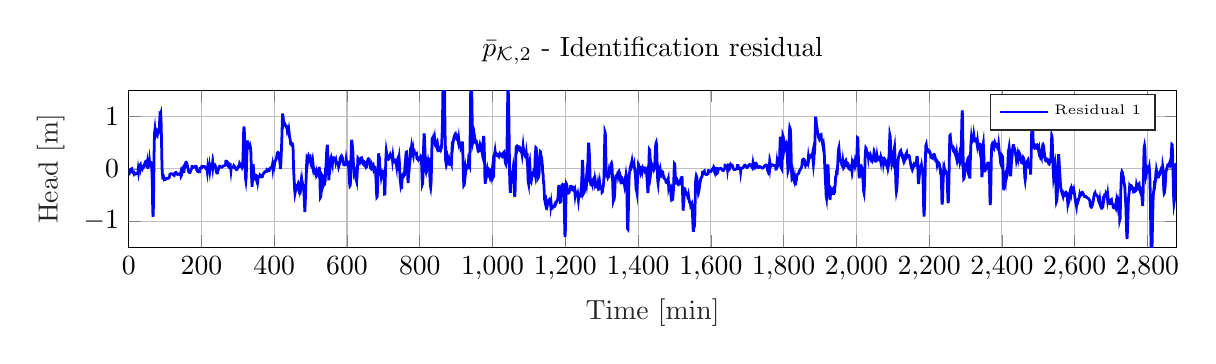
\begin{tikzpicture}

\begin{axis}[%
width=5.239in,
height=0.784in,
at={(0.815in,0.435in)},
scale only axis,
xmin=0,
xmax=2880,
xlabel style={font=\color{white!15!black}},
xlabel={Time [min]},
ymin=-1.5,
ymax=1.5,
ylabel style={font=\color{white!15!black}},
ylabel={Head  [m]},
axis background/.style={fill=white},
title style={},
title={$\bar{p}_{\mathcal{K},2}$ - Identification residual},
xmajorgrids,
ymajorgrids,
legend style={legend cell align=left, align=left, draw=white!15!black}
]
\addplot [color=blue, line width=1.0pt]
  table[row sep=crcr]{%
0	-0.123196861853295\\
1	-0.0986599217695456\\
2	-0.078665973862222\\
3	-0.0307880647171785\\
4	-0.0199247931497766\\
5	-0.012665686521018\\
6	-0.00744896580105348\\
7	-0.00309285824049965\\
8	0.000539057494442829\\
9	-0.0580977573863493\\
10	-0.0581814650881185\\
11	-0.0616373419378107\\
12	-0.0689236031769411\\
13	-0.0800300399209277\\
14	-0.094342085226252\\
15	-0.0775886499030278\\
16	-0.0915880829855524\\
17	-0.100640626112501\\
18	-0.103003954910491\\
19	-0.0994616974758955\\
20	-0.09316710236088\\
21	-0.0880310430939204\\
22	-0.0864386108272228\\
23	-0.0877873810843539\\
24	-0.0891185078356216\\
25	-0.0872833977039349\\
26	-0.022953042492091\\
27	-0.0709354905163195\\
28	-0.0266445627737895\\
29	-0.0144088133146809\\
30	0.0556890551328806\\
31	0.0674736336717601\\
32	0.0780848387022601\\
33	0.0246405237519625\\
34	0.0592035414268679\\
35	0.0545262819898724\\
36	0.0435229449062149\\
37	0.0284713187693555\\
38	0.00990846863695083\\
39	0.029895966810038\\
40	0.0242328580526561\\
41	0.0273416735713994\\
42	0.0439137472596016\\
43	0.0725477227443108\\
44	0.099817438245644\\
45	0.102098250731515\\
46	0.137469882467485\\
47	0.141985681361852\\
48	0.065271327928528\\
49	0.0565482019476278\\
50	0.048132752631119\\
51	0.0985022823306139\\
52	0.0287122688446075\\
53	0.0282224434788603\\
54	0.100732745672566\\
55	0.088012141094417\\
56	0.0953838470652428\\
57	0.151785605682193\\
58	0.079975053156943\\
59	0.0694926200867556\\
60	0.123673590765421\\
61	0.121844876021662\\
62	0.0615165991990878\\
63	0.039866758976224\\
64	-0.0928346978096073\\
65	-0.31154684952778\\
66	-0.805746755773583\\
67	-0.916185819940651\\
68	-0.723134333483671\\
69	-0.141657784219085\\
70	0.41867331586873\\
71	0.683054190705505\\
72	0.74324905846013\\
73	0.665968068070747\\
74	0.729281859660617\\
75	0.732883400206084\\
76	0.698980072360655\\
77	0.633250256435311\\
78	0.626842776453692\\
79	0.708489570276633\\
80	0.697101180924349\\
81	0.716485918923361\\
82	0.701487101565334\\
83	0.715794469720109\\
84	0.728674531001353\\
85	0.913781997916836\\
86	1.05261046788247\\
87	1.04669666586314\\
88	1.06628715229237\\
89	0.902675771488646\\
90	0.596852111855526\\
91	0.208521981109186\\
92	-0.0531337228566144\\
93	-0.125264251337583\\
94	-0.111448232674014\\
95	-0.124547401160193\\
96	-0.164023211115186\\
97	-0.192929222318604\\
98	-0.184638511713956\\
99	-0.200455270555779\\
100	-0.206832226614836\\
101	-0.20505623856387\\
102	-0.198233648956482\\
103	-0.190159240983711\\
104	-0.183963330858404\\
105	-0.181138605802616\\
106	-0.181318503006771\\
107	-0.182859133070501\\
108	-0.183704441518088\\
109	-0.181969879448737\\
110	-0.176392455264157\\
111	-0.166846623441721\\
112	-0.154705036553516\\
113	-0.109985664236319\\
114	-0.100207213828583\\
115	-0.0945508521259413\\
116	-0.0929842221368915\\
117	-0.0938848941118593\\
118	-0.0952199377223479\\
119	-0.0960548781431143\\
120	-0.0972276498274667\\
121	-0.100516040745582\\
122	-0.10696356381618\\
123	-0.115634422265281\\
124	-0.123582382049456\\
125	-0.127242496650723\\
126	-0.0920897261486573\\
127	-0.0840272334708203\\
128	-0.0745459026031057\\
129	-0.068637054834241\\
130	-0.0697406925332444\\
131	-0.0779905294754855\\
132	-0.090188720478622\\
133	-0.101473177617152\\
134	-0.107774254042901\\
135	-0.107779253476757\\
136	-0.103381869909079\\
137	-0.0984485770304957\\
138	-0.0966537007347625\\
139	-0.0996508113409718\\
140	-0.106492628138696\\
141	-0.111342162142265\\
142	-0.116608384372455\\
143	-0.0839376221582953\\
144	-0.137769051130121\\
145	-0.124217419992867\\
146	-0.0454868546230642\\
147	-0.0267984847051892\\
148	-0.0106513912652204\\
149	-0.06060089998698\\
150	-0.0554666350590551\\
151	-0.0544750539516059\\
152	-0.0535215642710511\\
153	0.013221454246839\\
154	0.0270314050223774\\
155	0.0804935049899527\\
156	0.103360029993809\\
157	0.120216418601103\\
158	0.125414348375827\\
159	0.117825594320657\\
160	0.0990297004876837\\
161	0.0706082841653668\\
162	0.035522831433326\\
163	-0.000678671368113726\\
164	-0.0318400899485098\\
165	-0.0544684259060588\\
166	-0.0680415963636634\\
167	-0.0733760978347249\\
168	-0.0711347976446959\\
169	-0.0617950895034198\\
170	-0.0465529888903902\\
171	-0.0280108559266949\\
172	-0.00975066313608153\\
173	0.00472835452103482\\
174	0.0453070326861891\\
175	0.0461524321140132\\
176	0.0410606680283863\\
177	0.0335298574429928\\
178	0.0277255687109985\\
179	0.0265139236704144\\
180	0.0302568957202496\\
181	0.0370877058800332\\
182	0.0438799035177908\\
183	0.04806194656787\\
184	0.0485080342643869\\
185	0.0454672996189416\\
186	0.0397715967665278\\
187	-0.0257799067862621\\
188	-0.0344918524069371\\
189	-0.0433678040232337\\
190	-0.0510487419423526\\
191	-0.0562472279721717\\
192	-0.0584294784953272\\
193	-0.0580712208222494\\
194	-0.056299460646791\\
195	-0.0542046731644916\\
196	0.00862012902964437\\
197	0.010291340660693\\
198	0.0120018304402336\\
199	0.0136947263745384\\
200	0.0148760565345754\\
201	0.0474419253102454\\
202	0.0464143434848125\\
203	0.0448633555284346\\
204	0.0437495206008123\\
205	0.0437462948338876\\
206	0.0446917124216526\\
207	0.0453931431605028\\
208	0.044021815271762\\
209	0.0390614570378673\\
210	0.0302706006427087\\
211	0.0189839158369622\\
212	0.00769390693344718\\
213	-0.000757517000145924\\
214	-0.00409277891371573\\
215	-0.00145905711100625\\
216	-0.0517914317787742\\
217	0.0164952810972565\\
218	-0.0314895057900557\\
219	-0.0242332632839037\\
220	-0.0209068172463489\\
221	-0.0211477101040032\\
222	0.0344702688961362\\
223	-0.0264786615937922\\
224	0.0318925736475251\\
225	0.0878946635149873\\
226	0.0863753267104173\\
227	0.0851855675084181\\
228	0.0262882321874827\\
229	0.0256358096275733\\
230	0.0833352860741883\\
231	0.0259285567140068\\
232	0.0864792140700388\\
233	0.0341821650064347\\
234	0.0427591361005355\\
235	0.0546652208764726\\
236	0.0672842052177387\\
237	0.0718493216069831\\
238	0.05458600801731\\
239	0.0156772955990618\\
240	-0.0298131060777322\\
241	-0.0628260795969737\\
242	-0.0785351713119979\\
243	-0.0810364153733971\\
244	-0.0778108214926547\\
245	-0.0385020423509843\\
246	-0.0237348086019722\\
247	0.000505596577170309\\
248	0.0266116272674637\\
249	0.0437915184437188\\
250	0.0490327279211513\\
251	0.0462208287997115\\
252	0.0402534785031889\\
253	0.0341614633049545\\
254	0.029901975735612\\
255	0.0288398735120907\\
256	0.0314221754751927\\
257	0.0370385759873102\\
258	0.0439753417600173\\
259	0.0501238482797248\\
260	0.0541141532043881\\
261	0.0560269298449043\\
262	0.057244745551202\\
263	0.059592495185214\\
264	0.0642684455222309\\
265	0.0710796430823351\\
266	0.0784326450953898\\
267	0.145090930358265\\
268	0.147428345433298\\
269	0.1458407242731\\
270	0.140803915411773\\
271	0.133352872035104\\
272	0.0666787537424156\\
273	0.0578282702259969\\
274	0.107557067417531\\
275	0.100317296719219\\
276	0.0943994145372073\\
277	0.0900741522271318\\
278	0.0874573054789494\\
279	0.0864008386918513\\
280	0.0286638481319415\\
281	-0.0308682244493994\\
282	0.0325997033365439\\
283	0.0358414105076506\\
284	0.0390770295674017\\
285	0.0412772045221033\\
286	0.0413777703995422\\
287	0.0386502559943978\\
288	0.0331148559574999\\
289	0.0580951058953687\\
290	0.0498014660902726\\
291	0.0411109598120092\\
292	0.0314208452622751\\
293	0.0198885318773137\\
294	0.00667572857635435\\
295	-0.0062627379584228\\
296	-0.015479599477402\\
297	-0.0173254024999352\\
298	-0.00986372793119727\\
299	0.00573725700565575\\
300	0.025215172087762\\
301	0.0429535952932554\\
302	0.0542396198352861\\
303	0.0570313811654799\\
304	0.0521772376237735\\
305	0.103422075345378\\
306	0.0920183131820309\\
307	0.0811679386253985\\
308	0.0719655986687968\\
309	0.0646395930102983\\
310	0.0644400343577871\\
311	0.0534720680985643\\
312	0.0298379420376804\\
313	0.0471084545705622\\
314	0.210548709058422\\
315	0.437874159416431\\
316	0.741567513871701\\
317	0.807671023803316\\
318	0.696255981063509\\
319	0.460078744566069\\
320	0.102047583890723\\
321	-0.179527437119845\\
322	-0.225970615856731\\
323	-0.151883894603735\\
324	0.106934551198506\\
325	0.307960692107379\\
326	0.454169979980762\\
327	0.542974266698138\\
328	0.4695075530325\\
329	0.43723196712056\\
330	0.41743761636544\\
331	0.422009146968875\\
332	0.426409929826363\\
333	0.406591619990763\\
334	0.430085925538833\\
335	0.399828639572178\\
336	0.289939506257731\\
337	-0.0235058625757958\\
338	-0.200322158722166\\
339	-0.343008678904631\\
340	-0.251717793988931\\
341	-0.0533915507679694\\
342	0.0901303489957144\\
343	0.00600284230264236\\
344	-0.124591739209471\\
345	-0.193725176683273\\
346	-0.19517509748848\\
347	-0.173078630328\\
348	-0.164929348820387\\
349	-0.164848057034739\\
350	-0.187703502567082\\
351	-0.129455073251208\\
352	-0.132871848067808\\
353	-0.140180769630824\\
354	-0.149705473420823\\
355	-0.216279910488304\\
356	-0.162817533102825\\
357	-0.162017499341431\\
358	-0.157316055951483\\
359	-0.152088432179397\\
360	-0.149887528016123\\
361	-0.121206410962152\\
362	-0.129541361523899\\
363	-0.14008325709424\\
364	-0.149666171098772\\
365	-0.15564504439012\\
366	-0.156721831991284\\
367	-0.153082700457006\\
368	-0.146027457045371\\
369	-0.104876424212911\\
370	-0.0960861623923321\\
371	-0.0850198329896799\\
372	-0.0774683925764208\\
373	-0.0698189848791628\\
374	-0.0618074906603852\\
375	-0.0540771309150969\\
376	-0.0478501797815838\\
377	-0.0442273667768589\\
378	-0.0437402828714824\\
379	-0.0462096715967562\\
380	-0.0183465438054498\\
381	-0.0239497729098517\\
382	-0.0296390786342116\\
383	-0.0346594796870647\\
384	-0.0380679926417855\\
385	-0.0387807887116765\\
386	-0.0362498109531728\\
387	0.00141880845152542\\
388	0.00789743645807306\\
389	0.0141661844534227\\
390	0.0193544446222873\\
391	0.0234120173447323\\
392	0.026938266036268\\
393	0.0305704587639042\\
394	0.0342470082464601\\
395	0.0726151127332102\\
396	0.013303313264764\\
397	0.0721993951141187\\
398	0.0769011476628378\\
399	0.0201613711885784\\
400	0.146609634479944\\
401	0.0987951886040292\\
402	0.142551151462051\\
403	0.153948747894887\\
404	0.166429907497871\\
405	0.182590379668603\\
406	0.204177008108999\\
407	0.229829260728962\\
408	0.287556774199928\\
409	0.306482189674369\\
410	0.313769714766657\\
411	0.306823782275544\\
412	0.286970524143548\\
413	0.290193233105207\\
414	0.208356669744838\\
415	0.154713554060358\\
416	0.0960949457798108\\
417	-0.00123765359153794\\
418	0.069944626570809\\
419	0.241015646050997\\
420	0.407290266365692\\
421	0.604510764279269\\
422	0.873615540918927\\
423	1.05676430337529\\
424	1.01258569953254\\
425	0.950014005164732\\
426	0.861006680042614\\
427	0.88547157168221\\
428	0.876306090939686\\
429	0.869174894575508\\
430	0.831137487054853\\
431	0.827259398124831\\
432	0.822088895983143\\
433	0.821745553873292\\
434	0.790386023793552\\
435	0.791820595422173\\
436	0.730375448802143\\
437	0.750671044990341\\
438	0.738193668855054\\
439	0.718335952174627\\
440	0.751764903443501\\
441	0.694378611289736\\
442	0.611470350050482\\
443	0.594309944839047\\
444	0.549150251922136\\
445	0.478118142218861\\
446	0.469100417934456\\
447	0.461505734091894\\
448	0.472385688137358\\
449	0.484752840026886\\
450	0.478811105141254\\
451	0.454656844818686\\
452	0.346742409119102\\
453	0.0340428551100231\\
454	-0.116443472595492\\
455	-0.261094949931746\\
456	-0.390944795038081\\
457	-0.470473077665311\\
458	-0.435858264623235\\
459	-0.386140141775201\\
460	-0.344567569215322\\
461	-0.357959071599922\\
462	-0.327835980510955\\
463	-0.329408705794265\\
464	-0.331835038819051\\
465	-0.308877002272283\\
466	-0.344716831573209\\
467	-0.299276587261716\\
468	-0.318971005118392\\
469	-0.34050522388096\\
470	-0.386308836184696\\
471	-0.341205019170388\\
472	-0.350384814491093\\
473	-0.291475279965617\\
474	-0.345774911146584\\
475	-0.307351887299042\\
476	-0.242679728970458\\
477	-0.304975792501878\\
478	-0.289594768347776\\
479	-0.323575560444858\\
480	-0.373468699876447\\
481	-0.399339433913887\\
482	-0.502049091497987\\
483	-0.632592914540076\\
484	-0.827210402002905\\
485	-0.694666443575983\\
486	-0.483499689276044\\
487	-0.289285701127874\\
488	-0.14358401724531\\
489	0.090748900821616\\
490	0.205263886921507\\
491	0.191966822615207\\
492	0.160512184521274\\
493	0.222448863464528\\
494	0.246016456869569\\
495	0.226667679301656\\
496	0.2358079762773\\
497	0.239130199913568\\
498	0.145553030773257\\
499	0.136530114797466\\
500	0.122922715600609\\
501	0.107222055835649\\
502	0.0600212374641842\\
503	0.0489460070587384\\
504	0.103928523379416\\
505	0.0418080584754392\\
506	0.0107398054654126\\
507	0.0719683914648783\\
508	0.0100005143904269\\
509	5.51746205132986e-05\\
510	-0.0477245101098873\\
511	-0.0660391612964588\\
512	-0.0837387234380316\\
513	-0.097528796280784\\
514	-0.10498141090914\\
515	-0.0766401275142599\\
516	-0.130718347683953\\
517	-0.118367230791449\\
518	-0.0997637805852492\\
519	-0.0829898100900479\\
520	-0.0667002837600705\\
521	-0.0881358482456349\\
522	-0.0125276794933669\\
523	0.0110815389017986\\
524	0.0121374423970835\\
525	-0.0787927249293432\\
526	-0.356763212302958\\
527	-0.544876815162141\\
528	-0.533058180846744\\
529	-0.430742450973504\\
530	-0.229395609798196\\
531	-0.120467208848588\\
532	-0.133145760458284\\
533	-0.23978865008376\\
534	-0.32516289617174\\
535	-0.300226059726704\\
536	-0.309787369788978\\
537	-0.298292128304823\\
538	-0.296848131611192\\
539	-0.201881650867072\\
540	-0.248232881321002\\
541	-0.0960069883139738\\
542	0.0181340259110101\\
543	0.160078484391555\\
544	0.318228769868632\\
545	0.399104497397303\\
546	0.458625147424172\\
547	0.323671197287283\\
548	0.166929342980893\\
549	-0.0286277300416344\\
550	-0.218137372222088\\
551	-0.0971205389032122\\
552	-0.0907059877261602\\
553	-0.00994838174910484\\
554	0.0907105454637502\\
555	0.16885657189917\\
556	0.196188723166763\\
557	0.151734059409286\\
558	0.140665268109721\\
559	0.14645001252002\\
560	0.108101138733943\\
561	0.193798989216283\\
562	0.185954234383289\\
563	0.203925431403846\\
564	0.210961361738818\\
565	0.206918217395753\\
566	0.195416608697293\\
567	0.181730759199532\\
568	0.169969052020747\\
569	0.130455865962574\\
570	0.159685128307615\\
571	0.125029454355499\\
572	0.120687772014129\\
573	0.114171217509437\\
574	0.107950743801233\\
575	0.106706932106448\\
576	0.0815492381380452\\
577	0.0398788050937497\\
578	0.0628687230274139\\
579	0.0884292617939835\\
580	0.11273636247823\\
581	0.193750320695742\\
582	0.208312672400126\\
583	0.184030902604071\\
584	0.185407580958\\
585	0.18012597568822\\
586	0.169263973429217\\
587	0.215940325832534\\
588	0.200760435333699\\
589	0.129371013112532\\
590	0.118897397937261\\
591	0.0793260149966528\\
592	0.0751397796377447\\
593	0.0737170118011363\\
594	0.0746359337913631\\
595	0.0783764733785333\\
596	0.0858322372014655\\
597	0.0969570569058007\\
598	0.171291615019406\\
599	0.12742643760032\\
600	0.106711534677466\\
601	0.116141039152701\\
602	0.127356231235176\\
603	0.128166034933024\\
604	0.0821814578598463\\
605	-0.0204228443213381\\
606	-0.148314882794253\\
607	-0.272464003292747\\
608	-0.325385475360044\\
609	-0.314413613933688\\
610	-0.164922727502493\\
611	0.147953835035118\\
612	0.475067334132184\\
613	0.557780810806548\\
614	0.485177904841485\\
615	0.426753490869061\\
616	0.358364918297369\\
617	0.181173968082234\\
618	0.0700509152594577\\
619	-0.0164738445815686\\
620	0.0232656019926338\\
621	0.00288187923462147\\
622	-0.0775298886035856\\
623	-0.0881256290829953\\
624	-0.173080526682739\\
625	-0.201514853577969\\
626	-0.159606481180766\\
627	-0.199016070311551\\
628	-0.0854796984396202\\
629	0.0525990213040473\\
630	0.202735566860127\\
631	0.193195576254944\\
632	0.143061567450296\\
633	0.125462797233787\\
634	0.140092982491034\\
635	0.125682786939564\\
636	0.150959910229574\\
637	0.176715552720459\\
638	0.19675914652575\\
639	0.208332788242565\\
640	0.211388884298628\\
641	0.175944156470152\\
642	0.16939964222459\\
643	0.103785947958386\\
644	0.0959615552358386\\
645	0.0884822771227292\\
646	0.0814963661851209\\
647	0.136491829726921\\
648	0.130657911579284\\
649	0.0915131416093189\\
650	0.0829432041466305\\
651	0.0735441783665891\\
652	0.0657124939531215\\
653	0.031205198430122\\
654	0.0384828870497813\\
655	0.0559286862677979\\
656	0.141163978546892\\
657	0.166362659081749\\
658	0.185724009243685\\
659	0.193956022154183\\
660	0.189949205382895\\
661	0.176219483971131\\
662	0.124140577810998\\
663	0.103267971194953\\
664	0.0852454074942841\\
665	0.0139841682676831\\
666	0.00605054192975274\\
667	0.0288167265245605\\
668	0.063412803105372\\
669	0.037581310722004\\
670	0.0474825538776145\\
671	0.0589552725517848\\
672	0.0694098972442205\\
673	0.0176127682079681\\
674	0.0434182936916088\\
675	0.0366811941186498\\
676	0.0320803617479228\\
677	-0.0190723639155905\\
678	-0.0260343929128481\\
679	-0.104424501922907\\
680	-0.263950680640534\\
681	-0.45320122147421\\
682	-0.541454886967209\\
683	-0.531619090630521\\
684	-0.382401480351994\\
685	-0.0738005327224158\\
686	0.165472942433574\\
687	0.296075536901263\\
688	0.197203945661769\\
689	0.200650097102162\\
690	0.0688380446188646\\
691	-0.0306930803198142\\
692	-0.0730732585471259\\
693	-0.0887042765608754\\
694	-0.150479287942154\\
695	-0.112394228226151\\
696	-0.0911846079699643\\
697	-0.124143763632205\\
698	-0.134182854822413\\
699	-0.140966404823651\\
700	-0.02364860683155\\
701	-0.126814455365697\\
702	-0.213803691033874\\
703	-0.484667759941331\\
704	-0.482754496962094\\
705	-0.281122263339562\\
706	0.000657608754444539\\
707	0.236135160047404\\
708	0.339238174919188\\
709	0.296668603408612\\
710	0.262688907011928\\
711	0.241208720315271\\
712	0.228513206996602\\
713	0.184629121621477\\
714	0.180760926128222\\
715	0.186297353198256\\
716	0.201454348884887\\
717	0.223872295928871\\
718	0.249230403821379\\
719	0.271503372517657\\
720	0.253116769959632\\
721	0.254076584133834\\
722	0.245652081905625\\
723	0.232376099398522\\
724	0.245696373241245\\
725	0.177225500549241\\
726	0.236166960455357\\
727	0.175798256603734\\
728	0.175093838621052\\
729	0.171070559473471\\
730	0.132448014295093\\
731	0.126421194608163\\
732	0.123643446994244\\
733	0.126308038622916\\
734	0.134796839005574\\
735	0.114734135859152\\
736	0.0678617821236855\\
737	0.199205070725625\\
738	0.146248191701055\\
739	0.115534784458887\\
740	0.173127499403421\\
741	0.158588107278689\\
742	0.166834150110354\\
743	0.210393435355833\\
744	0.117928330323707\\
745	-0.0253761331284466\\
746	-0.207492008148279\\
747	-0.24829374427739\\
748	-0.321322154158885\\
749	-0.295949159418015\\
750	-0.388068274932685\\
751	-0.239323666814279\\
752	-0.177859538391232\\
753	-0.13176213591305\\
754	-0.112095256095863\\
755	-0.118036828462756\\
756	-0.127823361005348\\
757	-0.10738762386886\\
758	-0.107439851987657\\
759	0.0308262734784819\\
760	0.124529357672635\\
761	0.177352239157663\\
762	0.291539063742668\\
763	0.320986391028697\\
764	0.323880432156159\\
765	0.192976519764379\\
766	0.0344108818807385\\
767	-0.181804414882826\\
768	-0.271140908393626\\
769	-0.127102040941558\\
770	-0.0801664872702688\\
771	-0.0115478023335456\\
772	0.121253179906901\\
773	0.149334477469765\\
774	0.274249004843476\\
775	0.408990766890376\\
776	0.332161491855871\\
777	0.394433064764108\\
778	0.334351890413615\\
779	0.334428422235973\\
780	0.33113450409072\\
781	0.298939147396069\\
782	0.360933592425027\\
783	0.310521183354211\\
784	0.378157016163662\\
785	0.294349787330255\\
786	0.301812877984091\\
787	0.305370173292111\\
788	0.303328721343128\\
789	0.294622131159976\\
790	0.279727137695374\\
791	0.286159729061254\\
792	0.205609215945401\\
793	0.190293189814433\\
794	0.182675818524473\\
795	0.183738469555315\\
796	0.191619866359567\\
797	0.169804596760976\\
798	0.17825262955887\\
799	0.182254382422563\\
800	0.182655123080075\\
801	0.204729429858396\\
802	0.215134932405086\\
803	0.24060783909372\\
804	0.232124666933785\\
805	0.104646346941855\\
806	-0.104915617260957\\
807	-0.298651876790565\\
808	-0.279069406740781\\
809	-0.110830638530985\\
810	0.235387885036815\\
811	0.542215533568545\\
812	0.676640833628575\\
813	0.609304789855806\\
814	0.401508934891716\\
815	0.118447179871715\\
816	-0.0145818297313483\\
817	-0.043984265764955\\
818	-0.00183551530152215\\
819	-0.00402791273497627\\
820	0.0785547744362205\\
821	0.0462149637566327\\
822	0.0872770644600678\\
823	0.135326923596061\\
824	0.096060471940099\\
825	0.213828396884168\\
826	0.111711798146658\\
827	-0.00423895695141852\\
828	-0.19352083745531\\
829	-0.315889371593194\\
830	-0.353681785783941\\
831	-0.279510168063311\\
832	-0.0520156397096301\\
833	0.322249827438128\\
834	0.576574522909432\\
835	0.588314863406907\\
836	0.55114295838986\\
837	0.476214187005112\\
838	0.54891396907059\\
839	0.517565868831284\\
840	0.514562129915426\\
841	0.562158887458772\\
842	0.487734729526991\\
843	0.443358327480503\\
844	0.438131021614282\\
845	0.442315500681353\\
846	0.422550187233576\\
847	0.497414102618485\\
848	0.512783089127659\\
849	0.46037874152816\\
850	0.428234173504137\\
851	0.422645410668316\\
852	0.414975020804974\\
853	0.34831131343919\\
854	0.347419754013217\\
855	0.379995527242571\\
856	0.384532222359056\\
857	0.394257048094488\\
858	0.372348903188346\\
859	0.394007600460156\\
860	0.449434127805091\\
861	0.596666637362688\\
862	0.779651167892226\\
863	1.19485906725428\\
864	1.71287835167101\\
865	2.18922688194593\\
866	2.3911548766821\\
867	2.23335442499301\\
868	1.70951866866104\\
869	0.978331557606325\\
870	0.450390488124377\\
871	0.163176695541296\\
872	0.11911461155065\\
873	0.159714462564303\\
874	0.213757194119239\\
875	0.151319051374514\\
876	0.184032803270625\\
877	0.126578717503364\\
878	0.104366811799387\\
879	0.0985057034189367\\
880	0.117937490337809\\
881	0.158193803854303\\
882	0.121841058050137\\
883	0.10668142357401\\
884	0.119694382739432\\
885	0.140637703729219\\
886	0.12875554466104\\
887	0.105462123527175\\
888	0.283969735032002\\
889	0.420445245323229\\
890	0.404110563886569\\
891	0.475763002656855\\
892	0.524429966655724\\
893	0.556954469765159\\
894	0.608852294074751\\
895	0.618387360154536\\
896	0.645296656267718\\
897	0.663248277716306\\
898	0.670406293873491\\
899	0.635960829663645\\
900	0.566626515519729\\
901	0.671398953475524\\
902	0.564525599454427\\
903	0.554875845892347\\
904	0.549986873217136\\
905	0.548122015606253\\
906	0.513724142368361\\
907	0.567798621479803\\
908	0.500804462704416\\
909	0.494387525595037\\
910	0.457294319930618\\
911	0.455225799448563\\
912	0.454621108911901\\
913	0.393319697851787\\
914	0.407609758227373\\
915	0.426631103843732\\
916	0.434718053549929\\
917	0.522227337974165\\
918	0.414568852725765\\
919	0.108408939828877\\
920	-0.168729543162442\\
921	-0.316868288823876\\
922	-0.305284222299584\\
923	-0.15774889360835\\
924	-0.0640568187650956\\
925	-0.00808898730310403\\
926	-0.0730038296675772\\
927	-0.0133310164087703\\
928	0.0130656022674671\\
929	0.0368268014754563\\
930	0.0287590904482329\\
931	0.0235944029252551\\
932	0.0536445996191404\\
933	0.0519725417773387\\
934	0.152758269622829\\
935	0.130336903212324\\
936	0.0933032644684246\\
937	0.0713287135185041\\
938	0.410582998162852\\
939	0.951229915663625\\
940	1.56647226420496\\
941	1.88242688865813\\
942	1.82120919483578\\
943	1.43805732674638\\
944	0.983674146850269\\
945	0.714825019096018\\
946	0.52167315475991\\
947	0.553951009974455\\
948	0.563837304558021\\
949	0.527401934972723\\
950	0.521363133062621\\
951	0.599393597424303\\
952	0.554590133897264\\
953	0.534011319033574\\
954	0.53956836369219\\
955	0.535893850229328\\
956	0.521162454560219\\
957	0.463418960952382\\
958	0.431210354213015\\
959	0.399367758805511\\
960	0.343438465276627\\
961	0.333431391013683\\
962	0.339808858228714\\
963	0.419007160105167\\
964	0.41697510302631\\
965	0.449135132929278\\
966	0.415023810927359\\
967	0.432181374994478\\
968	0.405723838223551\\
969	0.402746518415498\\
970	0.33496490181733\\
971	0.330601534601222\\
972	0.288904021463985\\
973	0.333956791549944\\
974	0.500423954668882\\
975	0.603468268118036\\
976	0.603020178749688\\
977	0.470167881101915\\
978	0.189862868168539\\
979	-0.176053911013092\\
980	-0.288266312135718\\
981	-0.16150495350881\\
982	-0.114513428366948\\
983	-0.0713015645583468\\
984	-0.0642988609910446\\
985	-0.0804322886019406\\
986	-0.0249055311780282\\
987	-0.0644174626128518\\
988	-0.0278115444965934\\
989	-0.0269767286994664\\
990	-0.0611759441764974\\
991	-0.0915810920486848\\
992	-0.0185467465462494\\
993	-0.024532454779667\\
994	-0.0763282838392669\\
995	-0.0249933253238481\\
996	-0.023317768491637\\
997	-0.0373429235419565\\
998	-0.0969377876843041\\
999	-0.0469135225144868\\
1000	0.0200371384119862\\
1001	-0.0462765179982085\\
1002	-0.15561316332581\\
1003	-0.141604435140721\\
1004	0.0648768751102722\\
1005	0.253707229483787\\
1006	0.295857649409932\\
1007	0.341866904345743\\
1008	0.285557677816414\\
1009	0.277665214581027\\
1010	0.288699089747468\\
1011	0.290554749414824\\
1012	0.285641344642009\\
1013	0.24752170891378\\
1014	0.244643207227064\\
1015	0.245383879761761\\
1016	0.25050294141986\\
1017	0.260705661062701\\
1018	0.243737049054545\\
1019	0.262704538293235\\
1020	0.282439193753646\\
1021	0.269482207116845\\
1022	0.281729342441601\\
1023	0.283260981130667\\
1024	0.274760623713348\\
1025	0.260478005322476\\
1026	0.247208746797412\\
1027	0.266865179219067\\
1028	0.272230618813097\\
1029	0.28735152503117\\
1030	0.273892532723565\\
1031	0.288774871880449\\
1032	0.231838411189521\\
1033	0.221708194316392\\
1034	0.198017033301383\\
1035	0.131480051618624\\
1036	0.095055186863398\\
1037	0.0816240132833315\\
1038	0.119830740426906\\
1039	0.221591251487311\\
1040	0.545558063770869\\
1041	1.04572601218307\\
1042	1.49882217897979\\
1043	1.55292840089293\\
1044	1.33996047898872\\
1045	0.958527437253544\\
1046	0.42917365586257\\
1047	-0.129882677660959\\
1048	-0.379864633613479\\
1049	-0.458162738409435\\
1050	-0.330592045364369\\
1051	-0.232334131306985\\
1052	-0.201392008497457\\
1053	-0.0978498595221993\\
1054	-0.0865937791011859\\
1055	-0.0518131000409312\\
1056	-0.0305008652760037\\
1057	0.0232044671746223\\
1058	-0.0379180204575533\\
1059	-0.168484031830992\\
1060	-0.466699378420067\\
1061	-0.53695534573059\\
1062	-0.448710329896009\\
1063	-0.144920042661781\\
1064	0.268515337934879\\
1065	0.419670600504062\\
1066	0.426108936590182\\
1067	0.400968122725658\\
1068	0.364403136529887\\
1069	0.388440400569472\\
1070	0.40597772196304\\
1071	0.393629103457386\\
1072	0.411220577420032\\
1073	0.420238676411977\\
1074	0.417043539689018\\
1075	0.40302937195743\\
1076	0.351892904413013\\
1077	0.335897886920257\\
1078	0.328785137559642\\
1079	0.334765602734521\\
1080	0.320584849800973\\
1081	0.278178663576412\\
1082	0.357458735105091\\
1083	0.367260101233342\\
1084	0.432784143185089\\
1085	0.368638018347475\\
1086	0.326502358447279\\
1087	0.312408457944692\\
1088	0.296141611910642\\
1089	0.27997722951055\\
1090	0.233412822576788\\
1091	0.22422909156731\\
1092	0.218795050708955\\
1093	0.286769727947636\\
1094	0.223573248981531\\
1095	0.297274181430701\\
1096	0.15510202557148\\
1097	-0.0625667864059594\\
1098	-0.247499112821032\\
1099	-0.282774965912722\\
1100	-0.104870712343775\\
1101	0.09223564113762\\
1102	0.126713009259696\\
1103	0.0140787390143444\\
1104	-0.161230939204295\\
1105	-0.239296264085652\\
1106	-0.252142706541335\\
1107	-0.203876363805691\\
1108	-0.132060602116837\\
1109	-0.147310433227396\\
1110	-0.130007409637159\\
1111	-0.0805504375359405\\
1112	-0.0664114761233492\\
1113	-0.0792513943662954\\
1114	-0.016763682897583\\
1115	-0.0168316949505467\\
1116	-0.0563688415058792\\
1117	0.18827069934413\\
1118	0.279327385676474\\
1119	0.403221674141697\\
1120	0.39559309795743\\
1121	0.301745410553224\\
1122	0.111898648490559\\
1123	-0.0576143286817086\\
1124	-0.19018966326442\\
1125	-0.178100273886088\\
1126	-0.164657699997363\\
1127	-0.150783319056153\\
1128	-0.0842803690286686\\
1129	0.104589803164082\\
1130	0.220217700127414\\
1131	0.331315567752903\\
1132	0.324504573470279\\
1133	0.257464016359549\\
1134	0.233043848708036\\
1135	0.209047598538689\\
1136	0.130794333850986\\
1137	0.0651197388642117\\
1138	-0.0764931384935323\\
1139	-0.106623343198933\\
1140	-0.264431444861863\\
1141	-0.27450356501744\\
1142	-0.429500492793075\\
1143	-0.586848618343311\\
1144	-0.60814438563991\\
1145	-0.660494648993648\\
1146	-0.686670048045322\\
1147	-0.656931456481153\\
1148	-0.751257251307557\\
1149	-0.75662468324176\\
1150	-0.726245229179249\\
1151	-0.686439790403867\\
1152	-0.655506172116418\\
1153	-0.635548796419549\\
1154	-0.656402676690249\\
1155	-0.653670867906655\\
1156	-0.657794386915867\\
1157	-0.666887101702237\\
1158	-0.6213186680096\\
1159	-0.635041590906319\\
1160	-0.709070719419877\\
1161	-0.658429565275931\\
1162	-0.725063905639274\\
1163	-0.757972078947326\\
1164	-0.754169312067631\\
1165	-0.747689930310095\\
1166	-0.740143597229483\\
1167	-0.732396398529772\\
1168	-0.724348719698042\\
1169	-0.71506625446969\\
1170	-0.70340309778797\\
1171	-0.688694420333817\\
1172	-0.671271201319563\\
1173	-0.684851467301336\\
1174	-0.666235650526815\\
1175	-0.648986022647719\\
1176	-0.633185116171603\\
1177	-0.618103661927769\\
1178	-0.601785705384458\\
1179	-0.591369126335174\\
1180	-0.544528572324651\\
1181	-0.423568955656144\\
1182	-0.311854250386446\\
1183	-0.36935821376111\\
1184	-0.435258228843175\\
1185	-0.561641322638145\\
1186	-0.638050458395796\\
1187	-0.63500774185993\\
1188	-0.515282084602539\\
1189	-0.422705697316665\\
1190	-0.402630620823714\\
1191	-0.310923925678587\\
1192	-0.304188351227658\\
1193	-0.322427524411971\\
1194	-0.314018219833869\\
1195	-0.311570538262629\\
1196	-0.447723782931398\\
1197	-0.686534477614991\\
1198	-1.001620320652\\
1199	-1.3043380513202\\
1200	-1.24472263550587\\
1201	-0.893703964983658\\
1202	-0.489919227673234\\
1203	-0.285069827565138\\
1204	-0.298651605818485\\
1205	-0.362353406152891\\
1206	-0.406988728734284\\
1207	-0.452339517495865\\
1208	-0.460671296037454\\
1209	-0.452812094014206\\
1210	-0.432591730485861\\
1211	-0.438238188933525\\
1212	-0.411322415375295\\
1213	-0.389236576609882\\
1214	-0.37442846737671\\
1215	-0.308728169933524\\
1216	-0.399880940450572\\
1217	-0.400260353758362\\
1218	-0.400795572071843\\
1219	-0.399398634816407\\
1220	-0.395080760340726\\
1221	-0.388135065209987\\
1222	-0.322747922910629\\
1223	-0.411171680909064\\
1224	-0.411302094770925\\
1225	-0.417247473474482\\
1226	-0.42767382333146\\
1227	-0.500682892843948\\
1228	-0.453316292176702\\
1229	-0.492948516787578\\
1230	-0.496651706604013\\
1231	-0.498524263802764\\
1232	-0.500499781124475\\
1233	-0.503175695328281\\
1234	-0.479588270836658\\
1235	-0.536851955082106\\
1236	-0.592909731666097\\
1237	-0.525544622256774\\
1238	-0.513062800331156\\
1239	-0.53288572082689\\
1240	-0.521906327529706\\
1241	-0.51250148817153\\
1242	-0.502631846530456\\
1243	-0.431615455787892\\
1244	-0.452087420201828\\
1245	-0.241169467435853\\
1246	-0.0745358610067726\\
1247	0.168270610743662\\
1248	0.100416627853853\\
1249	-0.106711338444654\\
1250	-0.351158017130743\\
1251	-0.459479388858725\\
1252	-0.446926092016035\\
1253	-0.411171261462819\\
1254	-0.35640982531249\\
1255	-0.35620801628734\\
1256	-0.312448134716838\\
1257	-0.266103126301125\\
1258	-0.183479440096839\\
1259	-0.241222932727887\\
1260	-0.16103558204027\\
1261	-0.171449708388053\\
1262	0.103443591701492\\
1263	0.36244182213786\\
1264	0.497850601000309\\
1265	0.434524021735648\\
1266	0.321024788569474\\
1267	0.111521561136122\\
1268	-0.126756769535902\\
1269	-0.247651893651081\\
1270	-0.290600099602308\\
1271	-0.28516543456324\\
1272	-0.27847214694247\\
1273	-0.271212508661485\\
1274	-0.295522763170233\\
1275	-0.227306323460652\\
1276	-0.214968666522104\\
1277	-0.202152852077326\\
1278	-0.28513094172888\\
1279	-0.279518030170657\\
1280	-0.279227461174756\\
1281	-0.224074171597834\\
1282	-0.284227453622393\\
1283	-0.257543282757169\\
1284	-0.314437074497512\\
1285	-0.31014578305976\\
1286	-0.309115627935491\\
1287	-0.313014966693501\\
1288	-0.352860708538309\\
1289	-0.359652508622474\\
1290	-0.303672656319236\\
1291	-0.359962883656507\\
1292	-0.34940457555637\\
1293	-0.368390682645185\\
1294	-0.355253613616455\\
1295	-0.286956772849116\\
1296	-0.340624338189699\\
1297	-0.36850722868806\\
1298	-0.365290505930929\\
1299	-0.362395877414421\\
1300	-0.358503331620661\\
1301	-0.446256406331194\\
1302	-0.437711443246847\\
1303	-0.36818773327272\\
1304	-0.345735603852461\\
1305	-0.299720338529823\\
1306	-0.201976128779073\\
1307	0.0557885725981606\\
1308	0.441032528088407\\
1309	0.707857995865936\\
1310	0.686875121751278\\
1311	0.377542088491985\\
1312	0.0577807891160873\\
1313	-0.0986283610177452\\
1314	-0.14423733560696\\
1315	-0.149674745693979\\
1316	-0.131139866529161\\
1317	-0.160645941497123\\
1318	-0.144260157385183\\
1319	-0.151543693185388\\
1320	-0.151956163984813\\
1321	-0.0521942273330112\\
1322	-0.077795381068789\\
1323	-0.082895772273595\\
1324	-0.0731453276793275\\
1325	-0.0189308551272944\\
1326	0.0963330597511742\\
1327	0.109267271914739\\
1328	0.0784696699397287\\
1329	-0.0337204615628934\\
1330	-0.213973966997031\\
1331	-0.438267169573756\\
1332	-0.616409902238459\\
1333	-0.595560984175712\\
1334	-0.587556372264572\\
1335	-0.544231948288463\\
1336	-0.427489469678839\\
1337	-0.25832627291549\\
1338	-0.171796770131273\\
1339	-0.137253557632384\\
1340	-0.135625070341703\\
1341	-0.127666333122789\\
1342	-0.149006923016081\\
1343	-0.144388347272901\\
1344	-0.0812600647248729\\
1345	-0.0712820075736715\\
1346	-0.147323436035599\\
1347	-0.124020348040858\\
1348	-0.100708432415701\\
1349	-0.145792173704756\\
1350	-0.174906915946544\\
1351	-0.127472629631193\\
1352	-0.149500518090214\\
1353	-0.176741428951843\\
1354	-0.202425688443739\\
1355	-0.195947089279876\\
1356	-0.267211320980579\\
1357	-0.268569442784177\\
1358	-0.262543635357936\\
1359	-0.250707800481884\\
1360	-0.26669502771761\\
1361	-0.246862991494083\\
1362	-0.286698513179175\\
1363	-0.207692289999947\\
1364	-0.186487931715327\\
1365	-0.206397425006124\\
1366	-0.167241081259576\\
1367	-0.114525431123546\\
1368	-0.16010557702473\\
1369	-0.347624801043054\\
1370	-0.751061845241644\\
1371	-1.14385316274195\\
1372	-1.15340411225446\\
1373	-0.935376398696114\\
1374	-0.529408194656611\\
1375	-0.238640094305268\\
1376	-0.101650397229662\\
1377	-0.0590794642099581\\
1378	0.00557133687890854\\
1379	0.0335734894555628\\
1380	0.0553366377387547\\
1381	0.10153957093344\\
1382	0.109187319176193\\
1383	0.144338889367297\\
1384	0.0837607331927615\\
1385	0.106748254938886\\
1386	0.089084927266228\\
1387	0.0633278220178326\\
1388	0.063749484247289\\
1389	0.0889848655317564\\
1390	0.0224854590819845\\
1391	-0.00878257720207642\\
1392	-0.0802891590278563\\
1393	-0.14172802005568\\
1394	-0.31940116732563\\
1395	-0.408391989034264\\
1396	-0.412215452923817\\
1397	-0.453507040025045\\
1398	-0.297530473804279\\
1399	-0.155460764305793\\
1400	0.00334881526506337\\
1401	0.0888514693272455\\
1402	0.0756762361623231\\
1403	-0.0132085497663752\\
1404	0.00439660605438519\\
1405	0.00729875555492043\\
1406	-0.029021692856368\\
1407	0.0225083424924648\\
1408	0.0186435261833253\\
1409	-0.0396128884502431\\
1410	-0.061895873596427\\
1411	0.0107972512885794\\
1412	0.0256505117680987\\
1413	0.00470790487030825\\
1414	0.0115729167467293\\
1415	0.0156188070110161\\
1416	0.0163869214640826\\
1417	-0.0111153106214061\\
1418	-0.00478637663659498\\
1419	-0.0589490235844892\\
1420	-0.0538738927687845\\
1421	-0.0296779912992662\\
1422	-0.0259483058196039\\
1423	-0.0160814397278202\\
1424	-0.129685874853571\\
1425	-0.235082534852566\\
1426	-0.333759869073667\\
1427	-0.464913976539329\\
1428	-0.388313149196662\\
1429	-0.175024066604777\\
1430	0.19728617873524\\
1431	0.370563151676507\\
1432	0.360411354072269\\
1433	0.224932186881276\\
1434	0.0231258443096607\\
1435	-0.0813842697770824\\
1436	-0.0339955753587375\\
1437	0.065511987689888\\
1438	0.0295522705014974\\
1439	0.0324735077968441\\
1440	0.0622573121256096\\
1441	0.0498677961853389\\
1442	0.0334279584521653\\
1443	0.0375821755720835\\
1444	-0.00156541841700175\\
1445	0.0169059286351327\\
1446	0.0915936544673173\\
1447	0.276170294240131\\
1448	0.421427090389507\\
1449	0.486214153755128\\
1450	0.504209048995364\\
1451	0.449556639111108\\
1452	0.220155064114365\\
1453	-0.0348672056311585\\
1454	-0.227539213798792\\
1455	-0.274262478803216\\
1456	-0.187387330976534\\
1457	-0.0643540215494554\\
1458	0.0078150484862789\\
1459	-0.00611587669725822\\
1460	-0.0800611365999515\\
1461	-0.0453612683518472\\
1462	-0.119522239980199\\
1463	-0.127103650844823\\
1464	-0.0677604014471669\\
1465	-0.0600374864175777\\
1466	-0.0823024795089182\\
1467	-0.0743529168070367\\
1468	-0.071341351679564\\
1469	-0.134265425062097\\
1470	-0.139038642207332\\
1471	-0.144735921724447\\
1472	-0.182470896437039\\
1473	-0.190570475111969\\
1474	-0.196720125792936\\
1475	-0.205459906489061\\
1476	-0.21636256441294\\
1477	-0.259265341229153\\
1478	-0.264617974063299\\
1479	-0.261525319476057\\
1480	-0.252557545421176\\
1481	-0.236573212963492\\
1482	-0.224630647394854\\
1483	-0.198570944025498\\
1484	-0.329989175440552\\
1485	-0.293863725484933\\
1486	-0.318136034482187\\
1487	-0.338149929994039\\
1488	-0.384236042805163\\
1489	-0.395615524515499\\
1490	-0.472331761198426\\
1491	-0.439565937682943\\
1492	-0.506925447370492\\
1493	-0.547300878544839\\
1494	-0.590232292657277\\
1495	-0.586372806673928\\
1496	-0.516019951664781\\
1497	-0.424778897364995\\
1498	-0.264608520714511\\
1499	-0.032809919780135\\
1500	0.0988414270181508\\
1501	0.090416581892832\\
1502	-0.0918234864175247\\
1503	-0.207814246222959\\
1504	-0.253167242938822\\
1505	-0.245017543518138\\
1506	-0.218941865428725\\
1507	-0.242006767783828\\
1508	-0.228703209657198\\
1509	-0.25033760388169\\
1510	-0.273581090908877\\
1511	-0.263562299829502\\
1512	-0.279001313481665\\
1513	-0.258734430374915\\
1514	-0.264797437805768\\
1515	-0.26430373711667\\
1516	-0.236239705408643\\
1517	-0.252271323179428\\
1518	-0.228104517447264\\
1519	-0.205071905833179\\
1520	-0.164369093608038\\
1521	-0.163796894502084\\
1522	-0.384383768421046\\
1523	-0.623755994517452\\
1524	-0.801085045414823\\
1525	-0.679945571807714\\
1526	-0.612573946102629\\
1527	-0.396609300851793\\
1528	-0.380607934015096\\
1529	-0.384177319844497\\
1530	-0.437019376320627\\
1531	-0.44687134424872\\
1532	-0.45045401007129\\
1533	-0.488621443999762\\
1534	-0.494173745940117\\
1535	-0.5032119330873\\
1536	-0.511093334514278\\
1537	-0.55406083314324\\
1538	-0.566956854567557\\
1539	-0.522949205606821\\
1540	-0.568047952090367\\
1541	-0.637732157808728\\
1542	-0.640803387143549\\
1543	-0.638899904100747\\
1544	-0.666710344108104\\
1545	-0.726154491642646\\
1546	-0.719829905359539\\
1547	-0.708184570371259\\
1548	-0.690935882072523\\
1549	-0.781421037672146\\
1550	-0.93803312261845\\
1551	-1.13490766184551\\
1552	-1.20333090144399\\
1553	-1.12752041743088\\
1554	-1.11571874882711\\
1555	-1.10274633561487\\
1556	-0.952502798736326\\
1557	-0.604485147362745\\
1558	-0.25533494260749\\
1559	-0.176836963700779\\
1560	-0.135905030210438\\
1561	-0.154180352089341\\
1562	-0.176688617778687\\
1563	-0.273531216630772\\
1564	-0.375198253265388\\
1565	-0.428277164645479\\
1566	-0.390127144980056\\
1567	-0.423250666673461\\
1568	-0.394350505194552\\
1569	-0.323741629687213\\
1570	-0.270843160053552\\
1571	-0.246986523941025\\
1572	-0.20422150019305\\
1573	-0.180444466770666\\
1574	-0.167207313875167\\
1575	-0.154347019629533\\
1576	-0.145914831433991\\
1577	-0.0857187758518023\\
1578	-0.0915838965512705\\
1579	-0.0930539434368853\\
1580	-0.0880671657624816\\
1581	-0.0479487583892109\\
1582	-0.0419465172530522\\
1583	-0.0973687110927273\\
1584	-0.0983144479604761\\
1585	-0.101589879265596\\
1586	-0.105389941124827\\
1587	-0.108182001283758\\
1588	-0.109228165207753\\
1589	-0.108447287127824\\
1590	-0.106056329333455\\
1591	-0.102513001411204\\
1592	-0.098646582529561\\
1593	-0.0346453405757359\\
1594	-0.0336769289761349\\
1595	-0.0357086571300869\\
1596	-0.0407617618919787\\
1597	-0.047493133000593\\
1598	-0.053438394072586\\
1599	-0.0558809901000004\\
1600	-0.0529206674903264\\
1601	-0.044268871217831\\
1602	-0.0314914048143109\\
1603	-0.0173736071402359\\
1604	-0.00478545047149481\\
1605	0.0041657199953633\\
1606	0.00823454013216463\\
1607	0.00681104076208783\\
1608	0.0322225452524378\\
1609	0.0199624714241722\\
1610	-0.0543626260453394\\
1611	-0.0725517316241522\\
1612	-0.0314062187327053\\
1613	-0.0406543362613547\\
1614	-0.0490870636900027\\
1615	-0.0475535994243188\\
1616	-0.098630211653024\\
1617	0.0297370635467971\\
1618	-0.0804042411215562\\
1619	-0.0742530581239507\\
1620	-0.0100711884208238\\
1621	-0.00780778444835306\\
1622	-0.00570768446458914\\
1623	-0.00270862455419518\\
1624	0.00128740331039268\\
1625	0.00542912747725666\\
1626	0.00838040996065814\\
1627	0.00895938524785578\\
1628	0.0064511756601604\\
1629	0.000610900681898841\\
1630	-0.00818532047790654\\
1631	-0.0186319754029824\\
1632	-0.028477429408845\\
1633	-0.0350314206603173\\
1634	-0.0359680207533017\\
1635	-0.0303415606547404\\
1636	-0.0194250042915272\\
1637	-0.00674305968534128\\
1638	0.00332980521934445\\
1639	0.0686061463885608\\
1640	0.066756643073532\\
1641	0.0609541614550224\\
1642	0.054619240991876\\
1643	0.0503874358187844\\
1644	0.0486928795833919\\
1645	0.0476941981664609\\
1646	-0.0131351944067006\\
1647	0.0390676624906661\\
1648	0.0641705158703942\\
1649	0.0583752618514453\\
1650	0.0571399552471163\\
1651	0.0619173377512539\\
1652	0.0723438635430895\\
1653	0.0288519476066753\\
1654	0.045209546278187\\
1655	0.0607855756042426\\
1656	0.0726118285636872\\
1657	0.077823255884212\\
1658	0.0744349732043048\\
1659	0.0622879712358184\\
1660	0.0436198098097194\\
1661	0.0226725025694492\\
1662	0.00410190439151847\\
1663	-0.00889850323586927\\
1664	-0.0155897011978539\\
1665	-0.0172360740748587\\
1666	-0.0158553929425764\\
1667	-0.0130419032303166\\
1668	-0.00957700558027597\\
1669	-0.00575877197564978\\
1670	-0.00196115699503707\\
1671	0.00118641451280155\\
1672	0.00305645952531108\\
1673	0.0644666548878021\\
1674	0.064166174926541\\
1675	0.0644276024581103\\
1676	0.00836000546194526\\
1677	0.0118779239679228\\
1678	0.0155969003561367\\
1679	0.0176970396078602\\
1680	0.01709520592388\\
1681	0.014109259643952\\
1682	-0.0509796024962625\\
1683	0.00647555151338253\\
1684	0.00492541755213693\\
1685	0.00568687127489653\\
1686	0.00836570909633849\\
1687	0.0126589850863184\\
1688	0.0188884604463126\\
1689	0.0276464554529312\\
1690	0.0389246664990921\\
1691	0.0514954944340644\\
1692	0.0629449483728237\\
1693	0.0703822503774916\\
1694	0.0716255086091451\\
1695	0.066249068308494\\
1696	0.0558489397780448\\
1697	0.0434041803041652\\
1698	0.0323273933332473\\
1699	0.0255844730251482\\
1700	0.0249771709001365\\
1701	0.0306481625885979\\
1702	0.0411418460378812\\
1703	0.0539521097365281\\
1704	0.0662619482909292\\
1705	0.075653931449331\\
1706	0.0807171200691954\\
1707	0.0812605716529973\\
1708	0.077996912752468\\
1709	0.0719764524444741\\
1710	0.0641598961168555\\
1711	0.0552106233105647\\
1712	0.0454086815160224\\
1713	0.0347380797480028\\
1714	0.0232863109184009\\
1715	0.0728984856132584\\
1716	0.0027828311192124\\
1717	0.0921321016458805\\
1718	0.0630975499943176\\
1719	-0.0120181677413385\\
1720	0.0660810461677315\\
1721	-0.00881646593015972\\
1722	0.099558227744069\\
1723	0.104412650267051\\
1724	0.106752336958664\\
1725	0.0983631844866366\\
1726	0.0840742650536583\\
1727	0.0663791608804445\\
1728	0.0483483850698789\\
1729	0.0334208298991783\\
1730	0.0245429791748109\\
1731	0.0228932050444541\\
1732	0.0272790461566146\\
1733	0.0345011139672167\\
1734	0.0407349149986231\\
1735	0.0431673830007782\\
1736	0.0411428212106628\\
1737	0.0358307795793991\\
1738	0.0290289396492867\\
1739	0.0222083108721094\\
1740	0.0164723332736187\\
1741	0.0129059236580744\\
1742	0.012284251919958\\
1743	0.0151382937811704\\
1744	0.0213305543588831\\
1745	0.0299519530879664\\
1746	0.0395701556031582\\
1747	0.0487692231752206\\
1748	0.0566840537337683\\
1749	0.063173991108556\\
1750	0.0684560485268193\\
1751	0.0724734052609293\\
1752	0.0744238424462438\\
1753	0.0728318452713665\\
1754	0.0661054608868952\\
1755	0.0534385151302743\\
1756	-0.0224211192032939\\
1757	-0.0429030181533321\\
1758	-0.0621923343403381\\
1759	-0.0440881059773162\\
1760	-0.022694878369947\\
1761	0.068173333468259\\
1762	0.0168351958066566\\
1763	0.0857151253077717\\
1764	0.0407979114350141\\
1765	0.0541520772755035\\
1766	0.0659176808144935\\
1767	0.0744168476049865\\
1768	0.0785225897401531\\
1769	0.0781162115868099\\
1770	0.0743062171653577\\
1771	0.0692319172691498\\
1772	0.0651612906425427\\
1773	0.0632907939547351\\
1774	0.0631103440620819\\
1775	0.0629677098075874\\
1776	0.0613384255999279\\
1777	0.0578962095751621\\
1778	0.0538245087693596\\
1779	-0.00662520554678281\\
1780	-0.00530507617003195\\
1781	0.0584971187923102\\
1782	0.128320713879937\\
1783	0.0793500104456655\\
1784	0.0852770456313365\\
1785	0.0920508460478047\\
1786	0.0796169815713412\\
1787	0.10574454250888\\
1788	0.0597610524898258\\
1789	0.208439723151336\\
1790	0.43803679932072\\
1791	0.615804249018055\\
1792	0.53558485501987\\
1793	0.261460798965679\\
1794	0.0121502108135729\\
1795	-0.00177445458561465\\
1796	0.192209967382226\\
1797	0.468712948551591\\
1798	0.634574643316597\\
1799	0.613165877671548\\
1800	0.549662278268464\\
1801	0.534472353714975\\
1802	0.440626254875085\\
1803	0.494285506674828\\
1804	0.493573622933354\\
1805	0.464180528047279\\
1806	0.525609787835805\\
1807	0.444117033536365\\
1808	0.466561479940353\\
1809	0.431827713771142\\
1810	0.328256064080364\\
1811	0.116261706178328\\
1812	-0.0398975817499689\\
1813	-0.015439848636305\\
1814	0.130820634149678\\
1815	0.45802867742762\\
1816	0.699856920528788\\
1817	0.791588445153309\\
1818	0.773224016829722\\
1819	0.722071065329715\\
1820	0.509697164295218\\
1821	0.179873298442423\\
1822	-0.0594406423447467\\
1823	-0.182426712467532\\
1824	-0.170026331244195\\
1825	-0.167704927410597\\
1826	-0.177349723381717\\
1827	-0.136495995404729\\
1828	-0.211033082696069\\
1829	-0.231112497632992\\
1830	-0.252932809092677\\
1831	-0.214028572848171\\
1832	-0.283643185659678\\
1833	-0.284848436680512\\
1834	-0.242923684021825\\
1835	-0.22526812130085\\
1836	-0.143175774047357\\
1837	-0.123659056581509\\
1838	-0.109119225644676\\
1839	-0.100113800243804\\
1840	-0.0948576267840267\\
1841	-0.0905359982205738\\
1842	-0.0847308344218902\\
1843	-0.0439370588978107\\
1844	-0.0335158130761002\\
1845	-0.0221771460175901\\
1846	-0.0106761444605112\\
1847	0.00118712117669162\\
1848	0.0141957211588633\\
1849	0.0288805626580171\\
1850	0.044882489847204\\
1851	0.121824832041014\\
1852	0.16838195530157\\
1853	0.178952526718298\\
1854	0.185019006207625\\
1855	0.186255410704433\\
1856	0.182571350016367\\
1857	0.173784430145943\\
1858	0.101869256938265\\
1859	0.0837579129499204\\
1860	0.0641316002638703\\
1861	0.0810741569525604\\
1862	0.0717962679490753\\
1863	0.0708152488755971\\
1864	0.0777008958597563\\
1865	0.0898159910525962\\
1866	0.135868075691455\\
1867	0.147676578452995\\
1868	0.217083069495772\\
1869	0.164568400237457\\
1870	0.201203724391569\\
1871	0.206152624020966\\
1872	0.212636943264357\\
1873	0.219076236527592\\
1874	0.222415935750234\\
1875	0.253932104134378\\
1876	0.250134284619321\\
1877	0.245564396396432\\
1878	0.240138045415655\\
1879	0.275793128235023\\
1880	0.310180812563367\\
1881	0.158006754350751\\
1882	0.0862813028227407\\
1883	0.150256507856973\\
1884	0.279133437891261\\
1885	0.303586994744876\\
1886	0.462387351203809\\
1887	0.766452685775924\\
1888	0.996204587759308\\
1889	0.953564533735396\\
1890	0.865427501106254\\
1891	0.810131180946918\\
1892	0.786704392448534\\
1893	0.716969098438646\\
1894	0.684402588453963\\
1895	0.655077925615409\\
1896	0.600758826492466\\
1897	0.589395220347427\\
1898	0.586027019373581\\
1899	0.561220765626651\\
1900	0.573061409267567\\
1901	0.584699812894037\\
1902	0.651087181838477\\
1903	0.654871280652358\\
1904	0.560495055998416\\
1905	0.555334997889226\\
1906	0.546266164504338\\
1907	0.470739518832609\\
1908	0.454322561928919\\
1909	0.406718916488813\\
1910	0.441241967462105\\
1911	0.380297397613148\\
1912	0.275011304332736\\
1913	0.0546079622117048\\
1914	-0.0713981786920925\\
1915	-0.243970716135593\\
1916	-0.346350300775526\\
1917	-0.52018861422242\\
1918	-0.558158415785279\\
1919	-0.420566788158929\\
1920	-0.174378972608451\\
1921	0.0294334227078323\\
1922	0.0847979907391405\\
1923	-0.0783976378470044\\
1924	-0.38738714905022\\
1925	-0.5043689899681\\
1926	-0.51131328811492\\
1927	-0.564832743014513\\
1928	-0.567444733999082\\
1929	-0.478906591768776\\
1930	-0.468421147155141\\
1931	-0.39161137757182\\
1932	-0.403789595561086\\
1933	-0.399330917186141\\
1934	-0.40512002657681\\
1935	-0.394614094387656\\
1936	-0.421601440271004\\
1937	-0.499385674592823\\
1938	-0.414699180624403\\
1939	-0.416359636315391\\
1940	-0.466036356806846\\
1941	-0.345886909519812\\
1942	-0.300235312672029\\
1943	-0.153167691276586\\
1944	-0.149760792993966\\
1945	-0.109140466297092\\
1946	-0.0151365781529051\\
1947	-0.112472764345291\\
1948	-0.00914833862928788\\
1949	0.124477797423573\\
1950	0.27756906721347\\
1951	0.377383025157933\\
1952	0.404902509885318\\
1953	0.321548546284909\\
1954	0.23499447003163\\
1955	0.16133408515018\\
1956	0.156055927850865\\
1957	0.142387867491927\\
1958	0.129573672418935\\
1959	0.117766288783166\\
1960	0.074639601372354\\
1961	0.0649413290358538\\
1962	0.117453488193803\\
1963	0.0207134359594221\\
1964	0.0758339003991324\\
1965	0.0208577515213264\\
1966	0.0318612986641895\\
1967	0.111913818251729\\
1968	0.103457935123551\\
1969	0.127863731017705\\
1970	0.147532761160647\\
1971	0.159251642941065\\
1972	0.12940111052292\\
1973	0.0668144874250984\\
1974	0.0590557780779477\\
1975	0.0523061963455405\\
1976	0.108514686034724\\
1977	0.10452462857991\\
1978	0.0424942309790808\\
1979	0.00516798616669689\\
1980	0.000259210096075435\\
1981	0.0542558354750042\\
1982	0.0522374997258126\\
1983	0.0552344061201637\\
1984	0.0294281342372003\\
1985	0.0367677816452527\\
1986	0.0440666919840567\\
1987	-0.00507588816851268\\
1988	0.0687104785530934\\
1989	0.0251811451593724\\
1990	0.107209449607836\\
1991	0.127477720481025\\
1992	0.110344071256016\\
1993	0.117560902650489\\
1994	0.058622521489383\\
1995	0.0472454158990985\\
1996	0.0994213266497255\\
1997	0.0499806385127002\\
1998	0.0728137303654748\\
1999	0.0590001469917496\\
2000	0.0671469360162433\\
2001	0.158912670969116\\
2002	0.380469771369029\\
2003	0.597400982329624\\
2004	0.592446198200904\\
2005	0.351126819184906\\
2006	0.138946374779287\\
2007	-0.065795583023224\\
2008	-0.180855841361698\\
2009	-0.0921006690675981\\
2010	-0.0119602048348852\\
2011	0.0168257665165683\\
2012	0.0562093630049887\\
2013	0.0603091525434536\\
2014	0.0434440500396178\\
2015	0.000387445279812937\\
2016	-0.112264652304439\\
2017	-0.144714017328752\\
2018	-0.196449437824576\\
2019	-0.311251411928673\\
2020	-0.428876519030851\\
2021	-0.459512990279521\\
2022	-0.344028215189105\\
2023	-0.0870791067768835\\
2024	0.190924405860095\\
2025	0.330949656754328\\
2026	0.400323647774989\\
2027	0.389625170629763\\
2028	0.334757010146497\\
2029	0.322374868273144\\
2030	0.312464602616231\\
2031	0.301527359114424\\
2032	0.293045261169098\\
2033	0.229218320348323\\
2034	0.286755343246895\\
2035	0.28386274411573\\
2036	0.27842331666448\\
2037	0.235546953208342\\
2038	0.219977637399907\\
2039	0.26168595258342\\
2040	0.243603550153409\\
2041	0.229568671155832\\
2042	0.167997453092916\\
2043	0.175615330989693\\
2044	0.159169924340318\\
2045	0.178258041950969\\
2046	0.195377077508624\\
2047	0.207404666110286\\
2048	0.274336894967824\\
2049	0.243635492649773\\
2050	0.275202000331738\\
2051	0.239765368199613\\
2052	0.20929930215614\\
2053	0.229209066798184\\
2054	0.2243186335443\\
2055	0.164769447991958\\
2056	0.170295461052547\\
2057	0.241590030497605\\
2058	0.200610634977764\\
2059	0.21608990560761\\
2060	0.225295042786016\\
2061	0.224691655236569\\
2062	0.183197956477024\\
2063	0.172178614120732\\
2064	0.165974774811119\\
2065	0.169331679510613\\
2066	0.182857397894871\\
2067	0.14438489898005\\
2068	0.224749638861773\\
2069	0.206017614723159\\
2070	0.211010190208349\\
2071	0.208049433162692\\
2072	0.200318367423698\\
2073	0.191811345502813\\
2074	0.127714311699052\\
2075	0.183712898485858\\
2076	0.187619466828465\\
2077	0.156535810964812\\
2078	0.186631195602708\\
2079	0.1783688826551\\
2080	0.131020389971631\\
2081	0.110828065383032\\
2082	0.0877310800478668\\
2083	0.0650233314980824\\
2084	0.0443852100420372\\
2085	0.0256605957948182\\
2086	0.0700139196753895\\
2087	0.0181212564198816\\
2088	0.0537980711803314\\
2089	0.16928322037981\\
2090	0.27187896604223\\
2091	0.482749868943664\\
2092	0.650457041741177\\
2093	0.619185458619469\\
2094	0.488727614457687\\
2095	0.313791494356458\\
2096	0.1687669242149\\
2097	0.110116633868863\\
2098	0.142775247502932\\
2099	0.127268619601324\\
2100	0.121632474360702\\
2101	0.103126946116561\\
2102	0.23005104771498\\
2103	0.324265869762449\\
2104	0.368458330268908\\
2105	0.410513935510593\\
2106	0.264136386192234\\
2107	0.111045646610151\\
2108	-0.136353648550589\\
2109	-0.352962365457643\\
2110	-0.435355210997734\\
2111	-0.399542198678681\\
2112	-0.301295395354593\\
2113	-0.120557646906335\\
2114	0.0587623467438405\\
2115	0.174098895902425\\
2116	0.221429867373239\\
2117	0.252984642927125\\
2118	0.255712939638229\\
2119	0.291851193640383\\
2120	0.319254001356562\\
2121	0.338461781406231\\
2122	0.347153692171936\\
2123	0.311579606572579\\
2124	0.297661373817256\\
2125	0.27563721111602\\
2126	0.24916764302219\\
2127	0.221766419746693\\
2128	0.197199176740646\\
2129	0.23996337843591\\
2130	0.230733749155455\\
2131	0.198606026450804\\
2132	0.146750030797271\\
2133	0.16237701366763\\
2134	0.180667798948946\\
2135	0.198659390235896\\
2136	0.276250082431929\\
2137	0.291503685546729\\
2138	0.305421337767761\\
2139	0.227207354314032\\
2140	0.237658984266879\\
2141	0.24628344844583\\
2142	0.25274582700321\\
2143	0.256068026716591\\
2144	0.2556482910014\\
2145	0.248695318013155\\
2146	0.23277442350021\\
2147	0.175326605723363\\
2148	0.142791990926938\\
2149	0.105245415540786\\
2150	0.0683650167951626\\
2151	0.037854643666023\\
2152	0.0429832678049635\\
2153	0.0101197187850275\\
2154	-0.0153672892295234\\
2155	0.00301147697003046\\
2156	0.0271725964224458\\
2157	0.0519707563553666\\
2158	0.0726988757284985\\
2159	0.0534282496237353\\
2160	0.0590060167082882\\
2161	0.0588508778640602\\
2162	0.0573749764241072\\
2163	0.0591401438477064\\
2164	0.0684964101033074\\
2165	0.13389613850137\\
2166	0.113077269308114\\
2167	0.242966561961531\\
2168	0.175739039529965\\
2169	0.0170590026710613\\
2170	-0.214886657824493\\
2171	-0.292213062708541\\
2172	-0.208300775490287\\
2173	-0.129875265839537\\
2174	-0.0661156571166828\\
2175	-0.0153498555458427\\
2176	0.0498252225325615\\
2177	0.0532467835330834\\
2178	0.0417385782359858\\
2179	0.07389970557319\\
2180	0.0275073286558296\\
2181	0.00951829568525397\\
2182	0.00252012187119277\\
2183	-0.149971750983163\\
2184	-0.412705050305874\\
2185	-0.760949788334479\\
2186	-0.913857579554879\\
2187	-0.781791433156918\\
2188	-0.522093849299232\\
2189	-0.131234522097742\\
2190	0.250190541604034\\
2191	0.444788117873344\\
2192	0.464816845990867\\
2193	0.405343692790119\\
2194	0.371401100972122\\
2195	0.363523678116636\\
2196	0.356307171853246\\
2197	0.359566459146599\\
2198	0.336308022524697\\
2199	0.344274268905991\\
2200	0.345348409790454\\
2201	0.336518650785848\\
2202	0.31914332468066\\
2203	0.297034696945353\\
2204	0.27522649078972\\
2205	0.224882275027277\\
2206	0.213342485293666\\
2207	0.209183791060759\\
2208	0.213271215125388\\
2209	0.226301798120147\\
2210	0.215016290866828\\
2211	0.240116096256045\\
2212	0.262711474622463\\
2213	0.276033537298481\\
2214	0.275325461109745\\
2215	0.260509848177612\\
2216	0.236449979699984\\
2217	0.210389706583697\\
2218	0.156859439360446\\
2219	0.144868030032967\\
2220	0.142215993465008\\
2221	0.146070319384329\\
2222	0.0925153660061966\\
2223	0.127458437956655\\
2224	0.129691965750574\\
2225	0.126513638783138\\
2226	0.118478734651774\\
2227	0.106324709483722\\
2228	0.0912484189176652\\
2229	0.0415016616252046\\
2230	0.0147070173467654\\
2231	-0.0546027488575191\\
2232	-0.0476463481718383\\
2233	-0.105292088475622\\
2234	-0.280430491026898\\
2235	-0.595363070204954\\
2236	-0.682347057382906\\
2237	-0.566122381918724\\
2238	-0.347887735979548\\
2239	-0.157495194664989\\
2240	-0.0217956119576144\\
2241	-0.0498079124910689\\
2242	-0.000976000593226445\\
2243	-0.0396348520554994\\
2244	-0.0454462624121916\\
2245	-0.0473636244340483\\
2246	-0.0454199552271959\\
2247	-0.0731983906611333\\
2248	-0.0890796715358135\\
2249	-0.0853628679202814\\
2250	-0.287424957572448\\
2251	-0.488017412881725\\
2252	-0.656675514981103\\
2253	-0.606698413914422\\
2254	-0.400392030295144\\
2255	-0.0422441004928942\\
2256	0.407304385626475\\
2257	0.635796734433143\\
2258	0.642774222288153\\
2259	0.561069768025583\\
2260	0.508172005666687\\
2261	0.45355808356414\\
2262	0.426928209604746\\
2263	0.408911055651288\\
2264	0.39827333834458\\
2265	0.39143894483955\\
2266	0.351422760306122\\
2267	0.340995255701934\\
2268	0.38618013277754\\
2269	0.373610304034003\\
2270	0.363561698167608\\
2271	0.324115360140617\\
2272	0.318906804442932\\
2273	0.253819083016914\\
2274	0.250875861899686\\
2275	0.217796922646102\\
2276	0.277945991165574\\
2277	0.224609034104596\\
2278	0.167909490827377\\
2279	0.193817117399284\\
2280	0.18829277271935\\
2281	0.177854450344263\\
2282	0.166880210897631\\
2283	0.219684516904493\\
2284	0.167414121980912\\
2285	0.212132046176514\\
2286	0.188023184664949\\
2287	0.296754933981347\\
2288	0.334474393167945\\
2289	0.628133033566677\\
2290	0.939297998390686\\
2291	1.11932364000106\\
2292	0.960323000131737\\
2293	0.415638493212569\\
2294	-0.00728483793201917\\
2295	-0.192860792968752\\
2296	-0.184296269340969\\
2297	-0.128104809284807\\
2298	-0.0612176118201972\\
2299	-0.027692797794252\\
2300	-0.021847328688736\\
2301	0.0714179303390949\\
2302	0.0663476101786245\\
2303	0.0937428500895052\\
2304	0.020553664962506\\
2305	-0.00614667479021591\\
2306	0.0805578654053605\\
2307	0.125553671131897\\
2308	0.179143394131529\\
2309	0.198885483673855\\
2310	0.0596391832682102\\
2311	-0.124757008822819\\
2312	-0.184727775071707\\
2313	0.0795491129572241\\
2314	0.313136710651207\\
2315	0.505874774575567\\
2316	0.587140006357835\\
2317	0.531929485168\\
2318	0.545529191526555\\
2319	0.566837642116447\\
2320	0.547031877999835\\
2321	0.559269449265749\\
2322	0.571873385958682\\
2323	0.642057607595575\\
2324	0.593766518580431\\
2325	0.506724954399886\\
2326	0.567986269138878\\
2327	0.568035688512182\\
2328	0.531515558821106\\
2329	0.52391266513466\\
2330	0.514771036678233\\
2331	0.505925585104656\\
2332	0.462832665068824\\
2333	0.518661141317736\\
2334	0.454974810472045\\
2335	0.453085242365006\\
2336	0.417787505432059\\
2337	0.413010337917058\\
2338	0.406835872727676\\
2339	0.365196881784897\\
2340	0.433652122328972\\
2341	0.462726780008602\\
2342	0.457789437307333\\
2343	0.324642371687354\\
2344	0.0631709861748107\\
2345	-0.159708162657779\\
2346	-0.0934510146699026\\
2347	0.19943652671482\\
2348	0.434372643731187\\
2349	0.479716497345919\\
2350	0.339042401183491\\
2351	0.142099701607336\\
2352	-0.0669316923233581\\
2353	-0.00694379818256863\\
2354	0.0563388876252304\\
2355	0.0597139978116346\\
2356	0.0371958102087149\\
2357	0.0449823733747294\\
2358	0.0200407951033625\\
2359	0.0326063836715775\\
2360	0.0524506488587733\\
2361	0.108191699038073\\
2362	0.108215997292277\\
2363	0.0814459966956633\\
2364	0.133149362673876\\
2365	-0.0950919743339043\\
2366	-0.174933808951259\\
2367	-0.543901828316223\\
2368	-0.69276288173365\\
2369	-0.579504945136506\\
2370	-0.191002372182275\\
2371	0.21129623031571\\
2372	0.448297012983446\\
2373	0.46554665619032\\
2374	0.440516629929967\\
2375	0.400321441980829\\
2376	0.420932606134286\\
2377	0.434288305624172\\
2378	0.418472071344077\\
2379	0.49557486721708\\
2380	0.514689612595859\\
2381	0.498685973647625\\
2382	0.450053948052904\\
2383	0.457638849450078\\
2384	0.460649560449134\\
2385	0.42723092963552\\
2386	0.420753055775116\\
2387	0.417373655403686\\
2388	0.417833666674873\\
2389	0.389626620213484\\
2390	0.394364302433075\\
2391	0.45142853340883\\
2392	0.378960991648817\\
2393	0.321230294906208\\
2394	0.283170298491349\\
2395	0.235644915020508\\
2396	0.151183150930898\\
2397	0.0922155938265234\\
2398	0.075397795940269\\
2399	0.120174409638764\\
2400	0.187655898450586\\
2401	0.242463912701297\\
2402	0.229931889914781\\
2403	0.0142577672826505\\
2404	-0.261329560642778\\
2405	-0.409443905258208\\
2406	-0.325085292484765\\
2407	-0.26206136965979\\
2408	-0.219563890780933\\
2409	-0.175259975390304\\
2410	-0.213719903175473\\
2411	-0.105469446904493\\
2412	-0.0944841017736664\\
2413	-0.0600169844873122\\
2414	-0.12982192225742\\
2415	-0.100488508267269\\
2416	0.00702340420532721\\
2417	0.206044376322517\\
2418	0.345992753267517\\
2419	0.365085362375766\\
2420	0.409705253633462\\
2421	0.347974431341449\\
2422	0.213157035690294\\
2423	-0.0293241734901457\\
2424	-0.143255754943688\\
2425	-0.021051966722375\\
2426	0.0901241068647067\\
2427	0.181257908396759\\
2428	0.235013600550211\\
2429	0.333462701899549\\
2430	0.421359177443883\\
2431	0.445868429731107\\
2432	0.445064886615057\\
2433	0.410871333704407\\
2434	0.402695619160397\\
2435	0.381513090808035\\
2436	0.352343352369488\\
2437	0.319901757312252\\
2438	0.257745945284285\\
2439	0.23713011344055\\
2440	0.16883151487913\\
2441	0.20112014082266\\
2442	0.222399702675268\\
2443	0.243917133211752\\
2444	0.209436570239475\\
2445	0.283978173723192\\
2446	0.257651974673983\\
2447	0.253127677019826\\
2448	0.240474752454261\\
2449	0.281960213524606\\
2450	0.266125450946198\\
2451	0.221794315297764\\
2452	0.153496930343941\\
2453	0.150163878784952\\
2454	0.116479525842543\\
2455	0.11459723905174\\
2456	0.110735974299168\\
2457	0.154224452151972\\
2458	0.162769360146996\\
2459	0.21265591195889\\
2460	0.201438535746348\\
2461	0.145659722579254\\
2462	-0.0314456635332974\\
2463	-0.162886468683979\\
2464	-0.212125640063121\\
2465	-0.150403039063768\\
2466	0.0158401150830869\\
2467	0.138962857861507\\
2468	0.0893957047051828\\
2469	0.102429596397101\\
2470	0.147507404071867\\
2471	0.160150256969224\\
2472	0.0809656173749573\\
2473	0.092716456306988\\
2474	0.0734300787537308\\
2475	0.0288901192310931\\
2476	0.019908117495568\\
2477	0.0388448812657103\\
2478	-0.0154618522457355\\
2479	-0.10833736397165\\
2480	0.0971991752636825\\
2481	0.410288151424481\\
2482	0.766324797030443\\
2483	0.966082870845447\\
2484	0.854969296020819\\
2485	0.729695268519784\\
2486	0.532469775590791\\
2487	0.462918785057418\\
2488	0.41520047830366\\
2489	0.397378097243212\\
2490	0.390329622880373\\
2491	0.394922289874998\\
2492	0.410046908241476\\
2493	0.43147047007453\\
2494	0.421669939062994\\
2495	0.441777845814727\\
2496	0.45579675645569\\
2497	0.460505732600552\\
2498	0.453984453083692\\
2499	0.435401167316655\\
2500	0.373692397117729\\
2501	0.339005555786244\\
2502	0.365950419263612\\
2503	0.276969587614722\\
2504	0.261532482824272\\
2505	0.255042862735692\\
2506	0.227289144902095\\
2507	0.242959632991671\\
2508	0.26872482938267\\
2509	0.242742610123948\\
2510	0.345549661982183\\
2511	0.388016787118062\\
2512	0.358332967545195\\
2513	0.428932080435807\\
2514	0.445012494507381\\
2515	0.423286667455699\\
2516	0.333349396129719\\
2517	0.290080157821386\\
2518	0.243302297380311\\
2519	0.210337458348356\\
2520	0.159660116364364\\
2521	0.151461232692995\\
2522	0.155208103227253\\
2523	0.166568568201853\\
2524	0.177857571529124\\
2525	0.182120469009682\\
2526	0.176544526062258\\
2527	0.12964090358706\\
2528	0.111418639622642\\
2529	0.0926787959817403\\
2530	0.0884424657557545\\
2531	0.114457414574915\\
2532	0.132916132696458\\
2533	0.14644588479311\\
2534	0.144734505627703\\
2535	0.245070507044858\\
2536	0.463290898043283\\
2537	0.6290013871429\\
2538	0.601914481925\\
2539	0.429600202537422\\
2540	0.139533052558775\\
2541	-0.0183021839305155\\
2542	-0.148022564793834\\
2543	-0.10121706632647\\
2544	-0.0621843558504551\\
2545	0.0563908615502129\\
2546	0.0979595913271751\\
2547	0.0222973865462492\\
2548	-0.20048168176524\\
2549	-0.463846314926094\\
2550	-0.626323271677393\\
2551	-0.606824241548573\\
2552	-0.509836289283882\\
2553	-0.404346189167519\\
2554	-0.115558762681125\\
2555	0.150867486976971\\
2556	0.280724030848724\\
2557	0.188567180823632\\
2558	0.0526712375610003\\
2559	-0.0638788224366635\\
2560	-0.174249665938468\\
2561	-0.291407399539487\\
2562	-0.374886832280794\\
2563	-0.415081515084538\\
2564	-0.43376051013712\\
2565	-0.453003130298789\\
2566	-0.475077042053641\\
2567	-0.497882106484951\\
2568	-0.521696004430112\\
2569	-0.484021276393285\\
2570	-0.503308922986541\\
2571	-0.514830985846537\\
2572	-0.51644110832811\\
2573	-0.508545063329095\\
2574	-0.495533125323185\\
2575	-0.450803013267439\\
2576	-0.446084271226852\\
2577	-0.453360255086764\\
2578	-0.474436285088501\\
2579	-0.508630139497079\\
2580	-0.549331765835831\\
2581	-0.644750517582601\\
2582	-0.601430554489802\\
2583	-0.650656194220275\\
2584	-0.627235331352765\\
2585	-0.595349940363072\\
2586	-0.553930846944205\\
2587	-0.507419715276079\\
2588	-0.466576144674008\\
2589	-0.378155371893413\\
2590	-0.363618854726184\\
2591	-0.416227502435575\\
2592	-0.357977059969208\\
2593	-0.359566015665514\\
2594	-0.419303924196704\\
2595	-0.422475630932283\\
2596	-0.430587891215147\\
2597	-0.447733654927042\\
2598	-0.415096324975849\\
2599	-0.455203018770035\\
2600	-0.504782705352021\\
2601	-0.55794640500622\\
2602	-0.607429346456669\\
2603	-0.647095566432576\\
2604	-0.672914559191959\\
2605	-0.712387828198843\\
2606	-0.649452594324643\\
2607	-0.63756115682839\\
2608	-0.618939874822715\\
2609	-0.628484430912003\\
2610	-0.603317219745712\\
2611	-0.578354910882716\\
2612	-0.556431284722109\\
2613	-0.539153012698691\\
2614	-0.494575271383802\\
2615	-0.518348284419041\\
2616	-0.509586382174412\\
2617	-0.498280520262966\\
2618	-0.483883324024163\\
2619	-0.467829703014417\\
2620	-0.454327101020638\\
2621	-0.448636750232041\\
2622	-0.453059409038325\\
2623	-0.466949413638403\\
2624	-0.486656269260848\\
2625	-0.506648463130489\\
2626	-0.521762893915316\\
2627	-0.529274136671653\\
2628	-0.530047948791392\\
2629	-0.527746231195046\\
2630	-0.526255598377205\\
2631	-0.528107042923352\\
2632	-0.53438986646907\\
2633	-0.543457606209074\\
2634	-0.552340418848189\\
2635	-0.558434211764023\\
2636	-0.561495906064692\\
2637	-0.563370220634212\\
2638	-0.567295636840676\\
2639	-0.575520120325059\\
2640	-0.588400359193081\\
2641	-0.60480093210424\\
2642	-0.622162826927877\\
2643	-0.701114544466591\\
2644	-0.719460986922606\\
2645	-0.73442489841176\\
2646	-0.736287389599191\\
2647	-0.723315985922703\\
2648	-0.703335964311407\\
2649	-0.683716940045962\\
2650	-0.657454008220483\\
2651	-0.617615289613546\\
2652	-0.568654570134044\\
2653	-0.523934359811506\\
2654	-0.490719154529216\\
2655	-0.469599999367773\\
2656	-0.458210489969552\\
2657	-0.486885667244565\\
2658	-0.488362207893999\\
2659	-0.493437526868156\\
2660	-0.500541681832054\\
2661	-0.508552465550281\\
2662	-0.520467019460924\\
2663	-0.528597573072688\\
2664	-0.545620648056826\\
2665	-0.562697040163634\\
2666	-0.614305408297426\\
2667	-0.633896514478685\\
2668	-0.651962004729022\\
2669	-0.608966412226401\\
2670	-0.681794372919171\\
2671	-0.692582289646069\\
2672	-0.703677587919437\\
2673	-0.714096531019166\\
2674	-0.753426265400606\\
2675	-0.753162871295238\\
2676	-0.742359642955968\\
2677	-0.719403420805982\\
2678	-0.627319688530761\\
2679	-0.645794867333571\\
2680	-0.599828119705386\\
2681	-0.555905603963701\\
2682	-0.519663814184092\\
2683	-0.527241835605828\\
2684	-0.515835859237392\\
2685	-0.516237435798708\\
2686	-0.467094825699377\\
2687	-0.479120891684595\\
2688	-0.48970547583631\\
2689	-0.495954114204316\\
2690	-0.560004604613255\\
2691	-0.501892124075432\\
2692	-0.568993427986285\\
2693	-0.613020756722058\\
2694	-0.629472221331298\\
2695	-0.649926133696958\\
2696	-0.663232682692737\\
2697	-0.668658364739507\\
2698	-0.665640126033026\\
2699	-0.599479820094551\\
2700	-0.590941782353987\\
2701	-0.586137090785449\\
2702	-0.648840746652709\\
2703	-0.657603640586061\\
2704	-0.671806242734093\\
2705	-0.688658286638741\\
2706	-0.73659210447066\\
2707	-0.746791825397231\\
2708	-0.74888880405004\\
2709	-0.745150643268978\\
2710	-0.731441338488139\\
2711	-0.714592426830265\\
2712	-0.731177947969492\\
2713	-0.685886530042971\\
2714	-0.70708424599453\\
2715	-0.636360438028937\\
2716	-0.681437864700605\\
2717	-0.60202641766422\\
2718	-0.581913476471676\\
2719	-0.629828539534373\\
2720	-0.625260681902901\\
2721	-0.567469795581452\\
2722	-0.567984932201838\\
2723	-0.74496698105672\\
2724	-0.973594919870607\\
2725	-0.946750044760762\\
2726	-0.672472524945213\\
2727	-0.401177768167194\\
2728	-0.195257100581692\\
2729	-0.0797678778972468\\
2730	-0.052828803022571\\
2731	-0.0659983682270919\\
2732	-0.0892082768229301\\
2733	-0.141269406097699\\
2734	-0.15999638856367\\
2735	-0.265864878087712\\
2736	-0.27323503305967\\
2737	-0.314071268463501\\
2738	-0.360265973543484\\
2739	-0.497249524212648\\
2740	-0.624931012981456\\
2741	-0.757854160951858\\
2742	-1.0449651695912\\
2743	-1.23757992818847\\
2744	-1.34290791751921\\
2745	-1.22118529579015\\
2746	-1.01781507791533\\
2747	-0.782239278513302\\
2748	-0.557166959921396\\
2749	-0.499382531865592\\
2750	-0.44543949619203\\
2751	-0.344726717824805\\
2752	-0.362408080914278\\
2753	-0.32342157963248\\
2754	-0.330935991864258\\
2755	-0.320222218275475\\
2756	-0.323541251382082\\
2757	-0.337810891341348\\
2758	-0.357107474685627\\
2759	-0.378486972953105\\
2760	-0.36270194113186\\
2761	-0.367441641351391\\
2762	-0.425655846038296\\
2763	-0.418507100962017\\
2764	-0.410169282271852\\
2765	-0.435333782703282\\
2766	-0.432155419903204\\
2767	-0.42506140182433\\
2768	-0.414321223564833\\
2769	-0.397670645534696\\
2770	-0.315911084748343\\
2771	-0.345040707406689\\
2772	-0.408190857607487\\
2773	-0.323433105268471\\
2774	-0.304790410320493\\
2775	-0.29769642463765\\
2776	-0.30276941340766\\
2777	-0.293585712392861\\
2778	-0.37469672662553\\
2779	-0.398899362500956\\
2780	-0.360513030114348\\
2781	-0.375888814246977\\
2782	-0.405134755103845\\
2783	-0.447782953739761\\
2784	-0.457544329399283\\
2785	-0.553270074897732\\
2786	-0.634975755085421\\
2787	-0.711399449776749\\
2788	-0.522032570629314\\
2789	-0.170986714979229\\
2790	0.176174034479004\\
2791	0.402262339950816\\
2792	0.437884614748064\\
2793	0.384336357351792\\
2794	0.167741136757648\\
2795	-0.0488665537051602\\
2796	-0.134994053085407\\
2797	-0.102855240544315\\
2798	-0.0711523487866685\\
2799	-0.0221433710102872\\
2800	-0.0234364437912475\\
2801	0.00402488636885323\\
2802	-0.00696325328537029\\
2803	-0.0209954070214664\\
2804	-0.00351163146110878\\
2805	0.0281339777637442\\
2806	-0.0635628358607789\\
2807	-0.22515829367142\\
2808	-0.564473001877957\\
2809	-1.05569959612341\\
2810	-1.49403388900134\\
2811	-1.75265563557308\\
2812	-1.69276985582869\\
2813	-1.41474040154356\\
2814	-1.05771338790693\\
2815	-0.757720665106568\\
2816	-0.5104633707587\\
2817	-0.437307293770282\\
2818	-0.409719836233606\\
2819	-0.314447452831516\\
2820	-0.328922400350478\\
2821	-0.276297233152022\\
2822	-0.223628007872932\\
2823	-0.115188612595716\\
2824	-0.127603239720017\\
2825	-0.0333483469643525\\
2826	-0.0696908432595791\\
2827	-0.0892861141512782\\
2828	-0.0852341001307764\\
2829	-0.0859113866356225\\
2830	-0.179358526914413\\
2831	-0.116543199989245\\
2832	-0.104367086606572\\
2833	-0.0851287174790514\\
2834	-0.0926321593979864\\
2835	-0.0652132980306064\\
2836	-0.0417682607548855\\
2837	-0.0205060385166931\\
2838	-0.0384601186502636\\
2839	-0.0304902913421188\\
2840	-0.0350327799936991\\
2841	-0.0580512405363862\\
2842	0.0446111230524053\\
2843	0.00146732898576118\\
2844	-0.21289679479127\\
2845	-0.412947060090772\\
2846	-0.466957820384202\\
2847	-0.453263616016251\\
2848	-0.385686973195753\\
2849	-0.298410580468214\\
2850	-0.183960634478666\\
2851	-0.0603277456402367\\
2852	-0.0271536224230431\\
2853	-0.013449884437037\\
2854	0.0325681762633963\\
2855	0.0411932522831009\\
2856	0.078583739299269\\
2857	0.0798431937918878\\
2858	0.0768520439786826\\
2859	0.0693210741308832\\
2860	0.0907684311200399\\
2861	0.113821517831006\\
2862	0.101733901413887\\
2863	0.0870198064479695\\
2864	0.124138978754971\\
2865	0.19624955091664\\
2866	0.331291391206641\\
2867	0.467636847837625\\
2868	0.461152396991864\\
2869	0.324502003294796\\
2870	0.0869688835635571\\
2871	-0.27712938614107\\
2872	-0.531199752668641\\
2873	-0.65433798317013\\
2874	-0.607617606408411\\
2875	-0.500624149473396\\
2876	-0.300011142055929\\
2877	-0.212192114647436\\
2878	-0.0634296216397559\\
2879	0.111051496651491\\
};
\addlegendentry{\tiny Residual 1}

\end{axis}
\end{tikzpicture}% 
  %\vspace{-2.5mm}
  \caption{Residual of the inlet pressure on data from period 1.}
  \label{fig:residual_pk2_p1}
  \end{figure}
 %\vspace{-8mm}
 \vspace{-3mm}

 %pk2_p2 - residual
  \begin{figure}[H]
  \centering
  %\hspace{0mm}
  %\includegraphics[width=0.35\textwidth]{report/pictures/missingfigure}
  % This file was created by matlab2tikz.
%
%The latest updates can be retrieved from
%  http://www.mathworks.com/matlabcentral/fileexchange/22022-matlab2tikz-matlab2tikz
%where you can also make suggestions and rate matlab2tikz.
%
\definecolor{mycolor1}{rgb}{0.00000,0.44700,0.74100}%
%
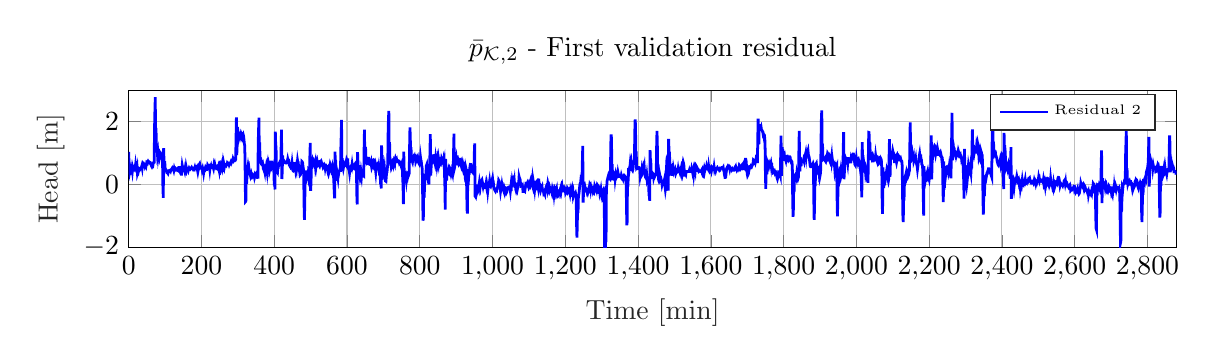
\begin{tikzpicture}

\begin{axis}[%
width=5.239in,
height=0.784in,
at={(0.94in,0.429in)},
scale only axis,
xmin=0,
xmax=2880,
xlabel style={font=\color{white!15!black}},
xlabel={Time [min]},
ymin=-2,
ymax=3,
ylabel style={font=\color{white!15!black}},
ylabel={Head  [m]},
axis background/.style={fill=white},
title style={},
title={$\bar{p}_{\mathcal{K},2}$ - First validation residual},
xmajorgrids,
ymajorgrids,
legend style={legend cell align=left, align=left, draw=white!15!black}
]
\addplot [color=blue, line width=1.0pt]
  table[row sep=crcr]{%
0	1.03916639511629\\
1	0.55522901414686\\
2	0.530057154498074\\
3	0.421708699705562\\
4	0.484870510880718\\
5	0.405440791981398\\
6	0.386938630284668\\
7	0.409202081908703\\
8	0.431431693494488\\
9	0.511618264279051\\
10	0.432019301171017\\
11	0.547558553222217\\
12	0.505480868327226\\
13	0.486736585343152\\
14	0.508755289704048\\
15	0.510337984950532\\
16	0.491484294629309\\
17	0.545845101707584\\
18	0.526916590867557\\
19	0.63034734629926\\
20	0.550381786494476\\
21	0.551737772607915\\
22	0.49185604105071\\
23	0.545985566729179\\
24	0.363627280738541\\
25	0.405623720657879\\
26	0.386380956572772\\
27	0.448695399886233\\
28	0.449769903441656\\
29	0.512001341646013\\
30	0.504645526410926\\
31	0.485194343380172\\
32	0.506499468848091\\
33	0.507361924715468\\
34	0.508180895067468\\
35	0.549755106298285\\
36	0.591285127235871\\
37	0.530772909266631\\
38	0.633174178119091\\
39	0.666222887043958\\
40	0.646374064945036\\
41	0.626479337614263\\
42	0.647337451097854\\
43	0.627349914745949\\
44	0.58691594133586\\
45	0.628032907194971\\
46	0.648702792323135\\
47	0.648925280514632\\
48	0.608300519479506\\
49	0.669624980964258\\
50	0.649302500872018\\
51	0.649330479381831\\
52	0.722560508682662\\
53	0.742888982218602\\
54	0.722368421745273\\
55	0.722197165723223\\
56	0.721975397473443\\
57	0.701303305291319\\
58	0.700979702559636\\
59	0.700604787860534\\
60	0.659379225086205\\
61	0.659485753888291\\
62	0.618791895297072\\
63	0.578096713307104\\
64	0.557799731923659\\
65	0.578300475163061\\
66	0.573260883331727\\
67	0.651750107150939\\
68	0.692646228337203\\
69	0.713141390331245\\
70	0.71323557721054\\
71	1.81490347306595\\
72	2.3485901585334\\
73	2.7824245429067\\
74	1.32554117394179\\
75	1.8019782664581\\
76	1.2940643928514\\
77	1.16010489648166\\
78	1.1793992555037\\
79	0.98081665954026\\
80	1.04270423211618\\
81	0.890470376291056\\
82	0.968829130169674\\
83	0.911708384685419\\
84	0.953271592473442\\
85	0.880240147217641\\
86	0.940322613883332\\
87	0.949718968420839\\
88	0.931728807056444\\
89	0.980116349390791\\
90	0.963699341905155\\
91	0.896298939103552\\
92	0.856358795415957\\
93	0.731334674018605\\
94	-0.101665730036387\\
95	-0.425117644748077\\
96	1.16203565930147\\
97	0.748371948441537\\
98	0.454479875603226\\
99	0.740119158002706\\
100	0.536167575491469\\
101	0.495410392737377\\
102	0.475050814433253\\
103	0.434289745297249\\
104	0.413926250073189\\
105	0.373161233530972\\
106	0.373193300466838\\
107	0.37322335570385\\
108	0.35285184409215\\
109	0.393676910509356\\
110	0.434499919860912\\
111	0.434521777080448\\
112	0.446594892806374\\
113	0.446612560600855\\
114	0.446628111237253\\
115	0.426241989765458\\
116	0.467052341265266\\
117	0.467061450846749\\
118	0.487467923650634\\
119	0.50787220484861\\
120	0.467075659643669\\
121	0.467073097036618\\
122	0.487469358945631\\
123	0.487465362587088\\
124	0.446661565180918\\
125	0.507854743950553\\
126	0.467049496122996\\
127	0.479095875364209\\
128	0.479088245996223\\
129	0.499479421733646\\
130	0.47907077981786\\
131	0.499460477493891\\
132	0.499449892010446\\
133	0.499438560619922\\
134	0.479026940578407\\
135	0.49941364914573\\
136	0.479000523585505\\
137	0.45858664116507\\
138	0.478971079155592\\
139	0.540153834832026\\
140	0.540137205473179\\
141	0.417722568361725\\
142	0.38895852827757\\
143	0.348140507486256\\
144	0.327721250813809\\
145	0.327700755558524\\
146	0.490875799022596\\
147	0.613250978512255\\
148	0.555237261314858\\
149	0.555213624515062\\
150	0.51439011568435\\
151	0.473565812145026\\
152	0.453140251223459\\
153	0.453113430250163\\
154	0.412286726559685\\
155	0.490648709423141\\
156	0.432628600386337\\
157	0.412199012593376\\
158	0.551519480228023\\
159	0.49349693012033\\
160	0.513863974130174\\
161	0.51383065688298\\
162	0.493396975746975\\
163	0.49336200809465\\
164	0.452764836802665\\
165	0.493289582752638\\
166	0.525704798144396\\
167	0.505504664453824\\
168	0.525627358679081\\
169	0.525587376962243\\
170	0.505147010458572\\
171	0.525504876575603\\
172	0.525462352725306\\
173	0.545818516324147\\
174	0.525374744793112\\
175	0.52532965555767\\
176	0.504884166047852\\
177	0.484437813698229\\
178	0.504789675947968\\
179	0.52514067024083\\
180	0.525091254025163\\
181	0.504835056257207\\
182	0.545769664863762\\
183	0.505098368849033\\
184	0.505218477583469\\
185	0.525730520799272\\
186	0.546235028585748\\
187	0.525932991384671\\
188	0.546422639985607\\
189	0.456560795941101\\
190	0.395437709985373\\
191	0.456704684242176\\
192	0.47716547084498\\
193	0.518018762251216\\
194	0.640463251237449\\
195	0.660903150894498\\
196	0.599738074622529\\
197	0.55896579612606\\
198	0.558985929409097\\
199	0.538599928770054\\
200	0.559006488796776\\
201	0.559007064361452\\
202	0.480610802062458\\
203	0.518190102984846\\
204	0.460180870449655\\
205	0.460156423328776\\
206	0.378527750201876\\
207	0.460089407539854\\
208	0.439647452061934\\
209	0.43959920073037\\
210	0.497536111748722\\
211	0.541483199538838\\
212	0.517810663805363\\
213	0.480148464322937\\
214	0.48007219629261\\
215	0.479990558988852\\
216	0.537894545922697\\
217	0.619162819876813\\
218	0.598666006679203\\
219	0.537602802179279\\
220	0.540465466639063\\
221	0.577944640188463\\
222	0.577827627255488\\
223	0.479153629113156\\
224	0.572440654380372\\
225	0.5602566678985\\
226	0.592573740537574\\
227	0.531472964394212\\
228	0.53132873892163\\
229	0.571741608366018\\
230	0.551189417202259\\
231	0.551032673942103\\
232	0.5508719196377\\
233	0.510145881787103\\
234	0.591337782652388\\
235	0.53020458643374\\
236	0.550428139331963\\
237	0.611209446702937\\
238	0.549827714023778\\
239	0.549641160442214\\
240	0.529051707734453\\
241	0.548924187949851\\
242	0.548256802534986\\
243	0.567877703996572\\
244	0.546617383096361\\
245	0.508112139655069\\
246	0.486774513087141\\
247	0.543831692134049\\
248	0.484939716454207\\
249	0.68488661601284\\
250	0.696186353356453\\
251	0.654748049771499\\
252	0.633848990963429\\
253	0.61311446177227\\
254	0.510970156595818\\
255	0.551833808917792\\
256	0.613092247144372\\
257	0.552681836917273\\
258	0.634865427611274\\
259	0.496627145051562\\
260	0.477646981443698\\
261	0.499786966426385\\
262	0.624021413668871\\
263	0.565480708161729\\
264	0.629217953741858\\
265	0.632357774491119\\
266	0.635867706401328\\
267	0.619352789590252\\
268	0.603215333306721\\
269	0.628255359933689\\
270	0.653672895786144\\
271	0.691518207204552\\
272	0.676881657387298\\
273	0.683008470572531\\
274	0.669091374506458\\
275	0.655519938230825\\
276	0.621882904138971\\
277	0.649765006734654\\
278	0.677952537971017\\
279	0.686029259020728\\
280	0.694376458301974\\
281	0.723373935559245\\
282	0.691402371773108\\
283	0.720836504648929\\
284	0.721707878033754\\
285	0.731084159647907\\
286	0.74059278408896\\
287	0.811405352402815\\
288	0.780297633172694\\
289	0.810437245008018\\
290	0.820196642275477\\
291	0.771955372415171\\
292	0.761263556636834\\
293	0.770899441195539\\
294	0.800832011289536\\
295	1.46301633067893\\
296	2.13685169593474\\
297	0.935312425069561\\
298	1.2210141079027\\
299	1.83577241749673\\
300	1.67432767896864\\
301	1.67435750465214\\
302	1.64864120245866\\
303	1.61426400071421\\
304	1.52280547030964\\
305	1.56957454374083\\
306	1.57625201716264\\
307	1.60049521753912\\
308	1.55038088184299\\
309	1.61714599615262\\
310	1.58628183579476\\
311	1.54358372892558\\
312	1.61860567351101\\
313	1.62565586439815\\
314	1.53862352048509\\
315	1.57245883333088\\
316	1.52042546457123\\
317	1.40019140511348\\
318	1.28602602966195\\
319	1.23345008514224\\
320	0.443251516825839\\
321	-0.545950894032096\\
322	-0.532152151720375\\
323	0.594714764191629\\
324	0.0225806531938346\\
325	0.216221383381814\\
326	0.600877418556848\\
327	0.515560014799831\\
328	0.592802073122833\\
329	0.521625958918271\\
330	0.55404055677834\\
331	0.44990120822581\\
332	0.354582795128586\\
333	0.328939604571573\\
334	0.303578190122799\\
335	0.258246086848963\\
336	0.295082983365013\\
337	0.344680124413614\\
338	0.3014602876206\\
339	0.332447417671808\\
340	0.314621922724541\\
341	0.254187675827971\\
342	0.268259756065646\\
343	0.251210033452033\\
344	0.268009264161762\\
345	0.294602286274241\\
346	0.223658754675206\\
347	0.265302612144744\\
348	0.296415647455696\\
349	0.320702751585365\\
350	0.301988206017356\\
351	0.296802432282078\\
352	0.33384922303248\\
353	0.273252354649181\\
354	0.284245139396532\\
355	0.185632193555342\\
356	1.32909314115403\\
357	1.78025436775187\\
358	2.12936351390997\\
359	0.784585204789622\\
360	1.34360448600407\\
361	0.763210734417974\\
362	0.726129279808042\\
363	0.704020590625248\\
364	0.726805895157966\\
365	0.644711364528412\\
366	0.63463991156771\\
367	0.658385454815253\\
368	0.679518797658417\\
369	0.607020950615514\\
370	0.504642263153592\\
371	0.484911029002603\\
372	0.450473779692686\\
373	0.470576621135287\\
374	0.40917509242967\\
375	0.54533251098939\\
376	0.528097026430693\\
377	0.508145209889072\\
378	0.575285249867818\\
379	0.505254222458674\\
380	0.423792588102508\\
381	0.608771626105849\\
382	0.672958303738\\
383	0.579296344724497\\
384	0.564642476496246\\
385	0.628023118466523\\
386	0.568044864941733\\
387	0.446531283990915\\
388	0.498349900532666\\
389	0.540596811827989\\
390	0.566215565464809\\
391	0.545301582653458\\
392	0.758764527795698\\
393	0.644240690991033\\
394	0.603021013778999\\
395	0.564356617284282\\
396	0.525816300166568\\
397	0.507750863940224\\
398	0.560007884624348\\
399	0.476136508607127\\
400	-0.0258877787073146\\
401	0.200071316623088\\
402	-0.159110363621117\\
403	1.68625602687356\\
404	1.27497088180482\\
405	1.19320619053612\\
406	0.504272712026051\\
407	0.442739527472831\\
408	0.406420831734764\\
409	0.385513656809493\\
410	0.524269113100061\\
411	0.531929711899963\\
412	0.617652433293273\\
413	0.654373419873721\\
414	0.681922095520342\\
415	0.660466642676155\\
416	0.684615958089964\\
417	0.642568939827463\\
418	0.646124541886508\\
419	1.22421381922617\\
420	1.74984828423799\\
421	0.176035798632647\\
422	0.418010236606506\\
423	0.926964747766824\\
424	0.688566730458092\\
425	0.728983712214657\\
426	0.730195903684283\\
427	0.751361985839523\\
428	0.733625949171902\\
429	0.7257953013196\\
430	0.701099111396715\\
431	0.690300391005017\\
432	0.685529169987014\\
433	0.697337533374608\\
434	0.701429621229643\\
435	0.702972598175094\\
436	0.743125043043456\\
437	0.805144528995974\\
438	0.747568076679094\\
439	0.725382535768425\\
440	0.736185200611281\\
441	0.629567350032382\\
442	0.616420012736199\\
443	0.589895747435932\\
444	0.566715890618859\\
445	0.545925873877735\\
446	0.56711305547384\\
447	0.612616105817956\\
448	0.579070513469148\\
449	0.677943555203349\\
450	0.579959256791774\\
451	0.459601078698505\\
452	0.437333813613009\\
453	0.428378566957029\\
454	0.437263935010279\\
455	0.46707393350939\\
456	0.713206356652819\\
457	0.586974237800469\\
458	0.593524777885378\\
459	0.481131536100314\\
460	0.545953507732087\\
461	0.488262879383228\\
462	0.613281179825954\\
463	0.658749419855965\\
464	0.767748240591494\\
465	0.698254665421508\\
466	0.69786250759023\\
467	0.559426744077648\\
468	0.525773436637287\\
469	0.427437010854156\\
470	0.399595259044666\\
471	0.297923264424313\\
472	0.311785573935062\\
473	0.38097050256399\\
474	0.521373712506666\\
475	0.575595952801649\\
476	0.730768312562354\\
477	0.719266622308901\\
478	0.696728405860355\\
479	0.575163153108797\\
480	0.517080941169652\\
481	0.290760072803209\\
482	-0.664940719166189\\
483	-1.12753940057267\\
484	-0.551532018023828\\
485	0.383961318449266\\
486	0.0265173851241229\\
487	0.444234824075728\\
488	0.363498956664671\\
489	0.271189131207478\\
490	0.321658410366069\\
491	0.298623035885448\\
492	0.308261450045265\\
493	0.247842847707354\\
494	0.400014669833375\\
495	0.368815083464156\\
496	0.427549430558678\\
497	0.428284718713385\\
498	0.927208578668697\\
499	1.32436398170543\\
500	-0.203213917476099\\
501	0.0328791651755225\\
502	0.499062090068925\\
503	0.564845165726851\\
504	0.651086452100721\\
505	0.716327275447519\\
506	0.646819017543805\\
507	0.662599774817053\\
508	0.709496965025139\\
509	0.66590370615976\\
510	0.702568724463134\\
511	0.683243125770794\\
512	0.724721892439653\\
513	0.599567265750395\\
514	0.67747389494599\\
515	0.58361205503347\\
516	0.668723956874253\\
517	0.68758007506856\\
518	0.735676715379981\\
519	0.671419904078988\\
520	0.629493061553809\\
521	0.647043001986454\\
522	0.644332507963512\\
523	0.622803479697659\\
524	0.728181922082243\\
525	0.735989386338318\\
526	0.740593656150345\\
527	0.674574972814099\\
528	0.717234171398438\\
529	0.737020220271006\\
530	0.699367541807291\\
531	0.64378817610681\\
532	0.639939521712897\\
533	0.598356239991432\\
534	0.556650978262198\\
535	0.581360921543926\\
536	0.623866641199349\\
537	0.641363292849839\\
538	0.617090833012675\\
539	0.558593654704509\\
540	0.661581117656603\\
541	0.521815495718876\\
542	0.564530396122848\\
543	0.580898634386052\\
544	0.555346235635163\\
545	0.530935871337839\\
546	0.508479884733802\\
547	0.527897733039438\\
548	0.365202625738931\\
549	0.327938563147825\\
550	0.375075568554259\\
551	0.416741444931795\\
552	0.422933845557395\\
553	0.55659896837664\\
554	0.641965053729329\\
555	0.608855152579878\\
556	0.604373522062055\\
557	0.519826307762678\\
558	0.446198629870075\\
559	0.471701516334562\\
560	0.409799628746093\\
561	0.53056128443005\\
562	0.477266300693721\\
563	0.500657287300854\\
564	0.00651131689279083\\
565	-0.253123841679383\\
566	-0.442995665272008\\
567	1.04934477731271\\
568	0.672976165611082\\
569	0.684448560608281\\
570	0.401495613325139\\
571	0.135746971233999\\
572	0.228857510118374\\
573	0.121194625033638\\
574	0.283640178360862\\
575	0.21359509790652\\
576	0.36795867242418\\
577	0.347086409327773\\
578	0.431197443016643\\
579	0.430752674021115\\
580	0.450721541415497\\
581	0.502920586122926\\
582	0.403729007640791\\
583	1.12937823375767\\
584	1.53699549986003\\
585	2.05922163637795\\
586	0.430892409965679\\
587	0.840120490540968\\
588	0.598680059852498\\
589	0.594894994453092\\
590	0.52311597003056\\
591	0.584929684419613\\
592	0.627986339996575\\
593	0.647535289857579\\
594	0.67082244720401\\
595	0.635922971675605\\
596	0.633080056396636\\
597	0.61744153961731\\
598	0.73998611677343\\
599	0.798789243547951\\
600	0.769676937286242\\
601	0.771845127904804\\
602	0.77597304536885\\
603	0.588178397654794\\
604	0.509834697412209\\
605	0.471838033808154\\
606	0.450909244742135\\
607	0.368383425060728\\
608	0.471553892423842\\
609	0.453753159466139\\
610	0.491083110013179\\
611	0.582658301564898\\
612	0.601436181742308\\
613	0.559640030479073\\
614	0.64524777453645\\
615	0.564437781409971\\
616	0.529229562055136\\
617	0.550534353273598\\
618	0.550843213421146\\
619	0.53184424875591\\
620	0.520111432362548\\
621	0.641743096921054\\
622	0.657089772227231\\
623	0.602040516186797\\
624	0.618917873879859\\
625	0.599575343727189\\
626	0.378340798052513\\
627	-0.332515867863485\\
628	-0.636936065410552\\
629	1.03132836246868\\
630	0.716058574447942\\
631	0.442498231465819\\
632	0.617727711271939\\
633	0.474910445193586\\
634	0.303347693730586\\
635	0.303090390104487\\
636	0.221471761764079\\
637	0.277512309625379\\
638	0.236692773114612\\
639	0.371123025013141\\
640	0.289504420371642\\
641	0.423934621029211\\
642	0.415567984501742\\
643	0.423656868559412\\
644	0.41849858517849\\
645	0.275681390150169\\
646	0.267314714237131\\
647	1.14447453109616\\
648	1.75106532575239\\
649	0.798270347618754\\
650	0.826234716210948\\
651	1.19977325205001\\
652	0.789892233174442\\
653	0.768375507229209\\
654	0.690399558829839\\
655	0.666112411752614\\
656	0.674190497221772\\
657	0.778581104047838\\
658	0.758623404454823\\
659	0.876662165657763\\
660	0.7624740763871\\
661	0.700370950583654\\
662	0.642661806512926\\
663	0.63933566210244\\
664	0.64426733141827\\
665	0.672029181984342\\
666	0.715135707972443\\
667	0.610113366811774\\
668	0.538662447610314\\
669	0.573394062418075\\
670	0.617349532387514\\
671	0.596321564048154\\
672	0.780857387770993\\
673	0.788452995173813\\
674	0.773522800121086\\
675	0.649821374216621\\
676	0.65035157000009\\
677	0.546398055489654\\
678	0.508321265329279\\
679	0.411879262136324\\
680	0.550631340053179\\
681	0.491846203229137\\
682	0.510353566683897\\
683	0.554544292323307\\
684	0.596902445927419\\
685	0.564849496350988\\
686	0.522027360400834\\
687	0.584753047171311\\
688	0.481492363186014\\
689	0.519094670996537\\
690	0.54618846738849\\
691	0.578366532279126\\
692	0.00575708396640806\\
693	0.128570949465939\\
694	-0.126834391647982\\
695	1.2470788054039\\
696	0.790036617975083\\
697	0.932930152659367\\
698	0.292298547135225\\
699	0.263656334103395\\
700	0.304561934322358\\
701	0.439122494716017\\
702	0.418599119464631\\
703	0.50031358023115\\
704	0.352498669205524\\
705	0.311822418654295\\
706	0.107953115062188\\
707	0.0997363571090872\\
708	0.262828367080587\\
709	0.397414866840464\\
710	0.400762340918263\\
711	0.53535532374616\\
712	0.637498749741802\\
713	1.63722521176484\\
714	2.11862014069654\\
715	2.34494561816564\\
716	0.954496182094154\\
717	1.3517622656944\\
718	0.762178609379554\\
719	0.705877125239496\\
720	0.670402437976108\\
721	0.629520299214931\\
722	0.529940446466611\\
723	0.558607753032192\\
724	0.698562580554068\\
725	0.719810501972162\\
726	0.760467789141877\\
727	0.749176762909293\\
728	0.667367699059952\\
729	0.730077748122206\\
730	0.691959829650017\\
731	0.658042647342477\\
732	0.798918331382176\\
733	0.840284289576836\\
734	0.804262347521245\\
735	0.796850212655627\\
736	0.813567775323797\\
737	0.749830890063357\\
738	0.74942872101137\\
739	0.722395665853881\\
740	0.723635125958666\\
741	0.726497512126151\\
742	0.752482601251089\\
743	0.747894851403295\\
744	0.693124209771192\\
745	0.712838398323136\\
746	0.697798757772873\\
747	0.676877957525555\\
748	0.621639477506506\\
749	0.582007332920647\\
750	0.623395881675066\\
751	0.545387236265384\\
752	0.52334688646026\\
753	0.210194765994366\\
754	-0.0368043702947887\\
755	-0.627030414578698\\
756	1.04809203194466\\
757	0.510037570126705\\
758	0.379985266666978\\
759	0.147946598652723\\
760	0.271057323339797\\
761	0.210583538202485\\
762	0.246981211721057\\
763	0.145494034390623\\
764	0.260304040045149\\
765	0.342672174344777\\
766	0.355506880713328\\
767	0.295100641993599\\
768	0.369156254043169\\
769	0.382024312076581\\
770	0.321414443252543\\
771	0.354704140750407\\
772	1.19537842039298\\
773	1.82003972483633\\
774	1.506734053667\\
775	0.79424992839256\\
776	1.19167747296714\\
777	0.783839284533599\\
778	0.783771541708397\\
779	0.746720485175167\\
780	0.714698612068254\\
781	0.795305406232828\\
782	0.807936695091122\\
783	0.809420958687646\\
784	0.86789334603715\\
785	0.847021817202361\\
786	0.88188829367364\\
787	0.82749986026618\\
788	0.847049992496025\\
789	0.726164776977619\\
790	0.756257301318804\\
791	0.82007563161595\\
792	0.855939053749879\\
793	0.856442342427997\\
794	0.880916722998322\\
795	0.80421772772101\\
796	0.76515503808421\\
797	0.685605107586774\\
798	0.664980816913037\\
799	0.739926964358787\\
800	0.726968396948912\\
801	0.723978554442148\\
802	0.864347939848017\\
803	0.773589710637978\\
804	0.751816020729798\\
805	0.628371391171164\\
806	0.569566382736198\\
807	0.470501576785303\\
808	-0.425912661598183\\
809	-1.15377582734135\\
810	-1.01576351403511\\
811	0.0289439175605608\\
812	-0.420067758448212\\
813	-0.122641447327382\\
814	0.142332320892876\\
815	0.235527821270182\\
816	0.317144167552328\\
817	0.349142532431657\\
818	0.593719857046608\\
819	0.625956598159348\\
820	0.465753056298794\\
821	0.273596345858344\\
822	0.285435748008481\\
823	0.142425695995676\\
824	0.0810145823708552\\
825	0.00241302820127487\\
826	0.340411172450708\\
827	0.433852500988777\\
828	1.04562932753798\\
829	1.60826157322848\\
830	0.286388848547453\\
831	0.448766532633897\\
832	0.892425504215268\\
833	0.748505903310665\\
834	0.735480599073057\\
835	0.837174865639717\\
836	0.83821983107196\\
837	0.918835128937616\\
838	0.920895999007975\\
839	0.890497939950343\\
840	0.763897022259457\\
841	0.744123091874904\\
842	0.68503049315273\\
843	0.785742803797994\\
844	0.654840142959777\\
845	0.771374952098256\\
846	0.769848377901965\\
847	0.65445216660423\\
848	0.751793216442742\\
849	0.657542716489907\\
850	0.717188036493241\\
851	0.658204384786195\\
852	0.796507323252477\\
853	0.721995433219689\\
854	0.743392536236321\\
855	0.660830542842234\\
856	0.69183585485159\\
857	0.690461985286909\\
858	0.669855931924424\\
859	0.709687210772465\\
860	0.809848668283117\\
861	0.773114920248354\\
862	0.697016598355809\\
863	0.694747733337266\\
864	0.677121392645027\\
865	0.752907646750771\\
866	0.6600234439601\\
867	0.722598234450736\\
868	0.35513049242924\\
869	-0.0375871050991634\\
870	-0.797312418467428\\
871	0.819499765857096\\
872	0.260233928693985\\
873	0.149758261107038\\
874	0.161680123246107\\
875	0.426742657516712\\
876	0.385812446049904\\
877	0.418134846490332\\
878	0.420976101618812\\
879	0.310502367702384\\
880	0.444823404364293\\
881	0.403894966649432\\
882	0.444565043981029\\
883	0.518007879118571\\
884	0.496923775081342\\
885	0.398006547669084\\
886	0.336680347165711\\
887	0.386197173171844\\
888	0.266881473764045\\
889	0.389152200576405\\
890	0.342852171331032\\
891	0.502714343902227\\
892	0.505797247142404\\
893	1.11765835961145\\
894	1.61917584063554\\
895	0.504682341959779\\
896	0.554334927310151\\
897	0.978714324321587\\
898	0.820574091013803\\
899	0.755464220427683\\
900	0.817153226054415\\
901	0.678730896402733\\
902	0.797447849892507\\
903	0.928732533953813\\
904	0.760913485417298\\
905	0.655974259352753\\
906	0.654464266301332\\
907	0.629798898896304\\
908	0.648693672237393\\
909	0.807150971337805\\
910	0.808268366829864\\
911	0.800035728667943\\
912	0.745483050882697\\
913	0.639527968115182\\
914	0.59737071798353\\
915	0.6549364404759\\
916	0.593706198054775\\
917	0.578398897298364\\
918	0.532503746680277\\
919	0.632655376992396\\
920	0.579100781051778\\
921	0.600546944662163\\
922	0.556023553688867\\
923	0.535934571174884\\
924	0.384356502417745\\
925	0.444752248856027\\
926	0.56260842799049\\
927	0.511382887867363\\
928	0.451325922296633\\
929	-0.164815158733916\\
930	-0.8185014575159\\
931	-0.925251142827165\\
932	0.488617409576605\\
933	-0.0146824401524697\\
934	0.187713794175707\\
935	0.31689281819795\\
936	0.335739947606911\\
937	0.485318766482699\\
938	0.573664022657596\\
939	0.641314979715709\\
940	0.639575932046419\\
941	0.605278895476026\\
942	0.463718720645296\\
943	0.408742991618368\\
944	0.406445919198511\\
945	0.391899409888254\\
946	0.458732871474759\\
947	0.435381986000493\\
948	0.521877506780832\\
949	0.45792873880719\\
950	1.02778357504909\\
951	1.30902186188167\\
952	-0.368955981192187\\
953	-0.386650670021311\\
954	0.00207938891963266\\
955	-0.219942345623203\\
956	-0.194963617954528\\
957	-0.254538961074729\\
958	-0.209072966359194\\
959	-0.177493888251064\\
960	-0.146558965551748\\
961	-0.0907551149003609\\
962	-0.133018437283845\\
963	-0.0100289031462566\\
964	0.0748556152786435\\
965	0.00264403489150311\\
966	-0.055685749995213\\
967	0.0672946354737931\\
968	0.11168221100268\\
969	0.114610090382122\\
970	0.115413599835939\\
971	0.139245034277344\\
972	0.0815225030927493\\
973	-0.00170946492652035\\
974	-0.0621021619034607\\
975	-0.00401686191790418\\
976	-0.0113336702253193\\
977	-0.0450174154011691\\
978	-0.0228308540518967\\
979	-0.0373563125944756\\
980	-0.0846551151123833\\
981	-0.0784002494814544\\
982	-0.000472960818761692\\
983	-0.0601356299244671\\
984	0.0220292345167508\\
985	-0.0502841870417257\\
986	-0.0706771938860342\\
987	-0.198962178361576\\
988	-0.095187915488566\\
989	-0.084891302245552\\
990	-0.0491204540760819\\
991	0.0335258410169388\\
992	0.112779951006949\\
993	0.0217434218706742\\
994	-0.0412162569350656\\
995	-0.0600743450636969\\
996	-0.0214488043810235\\
997	0.0228557719664195\\
998	0.128395132160968\\
999	0.149578269764383\\
1000	0.198624518168295\\
1001	0.0963270777403054\\
1002	0.0927393407293522\\
1003	-0.048522498376343\\
1004	-0.113261045226601\\
1005	-0.153317754412349\\
1006	-0.159228673512871\\
1007	-0.196739265419424\\
1008	-0.215609948275294\\
1009	-0.180179953988102\\
1010	-0.156326556886562\\
1011	-0.148047343922933\\
1012	-0.165112007556637\\
1013	-0.103689160742121\\
1014	-0.0812531209035399\\
1015	-0.000451095727527218\\
1016	-0.0172816116210868\\
1017	0.133547500617546\\
1018	0.112610418626268\\
1019	0.0489665417738152\\
1020	-0.0979209537814683\\
1021	-0.12122411600096\\
1022	-0.217999453865971\\
1023	-0.141758097136496\\
1024	-0.120344031163562\\
1025	-0.10320849296631\\
1026	-0.010591936305417\\
1027	-0.0783027124404825\\
1028	-0.0963589723639728\\
1029	-0.133412450717024\\
1030	-0.191621012755512\\
1031	-0.214198534386256\\
1032	-0.24899085701869\\
1033	-0.128761803789168\\
1034	-0.164283616096462\\
1035	-0.150127804916082\\
1036	-0.208090970961976\\
1037	-0.228461098955449\\
1038	-0.267981595906242\\
1039	-0.244522817051397\\
1040	-0.178646494190765\\
1041	-0.118751948809567\\
1042	-0.10014435967885\\
1043	-0.0998730238732506\\
1044	-0.0817217857522223\\
1045	-0.0784215536132322\\
1046	-0.0761007150392246\\
1047	-0.0980251901223639\\
1048	-0.130454973343113\\
1049	-0.209896925737823\\
1050	-0.105054113904814\\
1051	-0.212293971318047\\
1052	-0.052648183364056\\
1053	-0.0135757608268676\\
1054	0.113114556811993\\
1055	0.0526929055250349\\
1056	0.0947814511260958\\
1057	0.0121726088436844\\
1058	-0.00566078686970428\\
1059	0.0107003908126515\\
1060	0.088901813348258\\
1061	-0.0605166385016318\\
1062	-0.0623253224619518\\
1063	-0.047177543623782\\
1064	-0.164562203318965\\
1065	-0.205855018225058\\
1066	-0.168995537978837\\
1067	-0.120166297982308\\
1068	-0.16274701048696\\
1069	-0.10502136642976\\
1070	-0.0173917500570013\\
1071	0.0417874909939897\\
1072	0.0582602101685836\\
1073	0.251428362695627\\
1074	0.205279487962478\\
1075	0.189192214021894\\
1076	0.148650029073657\\
1077	0.00957313768359569\\
1078	-0.0553850918029539\\
1079	-0.0500913099840261\\
1080	-0.0334656185852893\\
1081	-0.0488066637552791\\
1082	-0.0312624430868382\\
1083	-0.116999121139365\\
1084	-0.261450668902043\\
1085	-0.160262088736118\\
1086	-0.146664014363878\\
1087	-0.165442298020913\\
1088	-0.068496931976064\\
1089	-0.0661164514390435\\
1090	-0.10722964114079\\
1091	-0.0307529129161708\\
1092	-0.0534999560448952\\
1093	-0.0543452710708436\\
1094	0.00475212285696358\\
1095	0.0459847495182686\\
1096	0.0604984332035059\\
1097	0.0835949626852965\\
1098	0.0575395643226315\\
1099	-0.0618732363536125\\
1100	-0.107602002193779\\
1101	-0.0870123688772821\\
1102	-0.0934183403029536\\
1103	-0.00937734457384209\\
1104	0.112458347237478\\
1105	0.149858374808467\\
1106	0.0653884384857122\\
1107	0.0393838600338583\\
1108	0.06582185444271\\
1109	-0.000844273412397456\\
1110	-0.0423024078922722\\
1111	0.172658992602422\\
1112	0.103242580791182\\
1113	0.0713397626809567\\
1114	0.0218628498632967\\
1115	-0.0386764757298224\\
1116	-0.137637453766679\\
1117	-0.0270814206130154\\
1118	-0.0395531979363781\\
1119	0.0614295947259365\\
1120	0.0753902353565294\\
1121	-0.00598565499451098\\
1122	-0.050114481634246\\
1123	-0.0131138829361106\\
1124	-0.0299911442499763\\
1125	-0.0874301281255896\\
1126	0.148487444188582\\
1127	0.146962904604905\\
1128	0.0457612332091628\\
1129	0.0241100317694531\\
1130	-0.0225420255327506\\
1131	-0.14719042573082\\
1132	-0.195085558774167\\
1133	-0.150667205907418\\
1134	-0.112582865389662\\
1135	-0.0787713517427164\\
1136	-0.0545621232300988\\
1137	-0.158426445131695\\
1138	-0.164511139384928\\
1139	-0.180990738330244\\
1140	-0.223929512005853\\
1141	-0.30389630710615\\
1142	-0.291025770784856\\
1143	-0.289387056403633\\
1144	-0.317479827664151\\
1145	-0.196791345775985\\
1146	-0.204450655900331\\
1147	-0.095945094236086\\
1148	-0.0624967251450315\\
1149	-0.0813027353016125\\
1150	-0.126249690394637\\
1151	-0.0424384889448248\\
1152	-0.138673252873559\\
1153	-0.072654919757305\\
1154	-0.14897810888678\\
1155	-0.11098244031291\\
1156	-0.157811317520739\\
1157	-0.0967192403659212\\
1158	-0.1410462609959\\
1159	-0.107402705866278\\
1160	-0.120827835438305\\
1161	-0.19097344101246\\
1162	-0.211758423717356\\
1163	-0.25659813619518\\
1164	-0.175919815623288\\
1165	-0.23879911332341\\
1166	-0.185077047646473\\
1167	-0.225159569478379\\
1168	-0.201899998707312\\
1169	-0.311044921951058\\
1170	-0.210806399770505\\
1171	-0.25160858552691\\
1172	-0.129707587115412\\
1173	-0.152063524009044\\
1174	-0.131837944628096\\
1175	-0.201135426135373\\
1176	-0.158164404552359\\
1177	-0.322263024457556\\
1178	-0.366333853008499\\
1179	-0.347690737712547\\
1180	-0.31078325288064\\
1181	-0.329522485026537\\
1182	-0.228506436154092\\
1183	-0.201440099935347\\
1184	-0.182135793177281\\
1185	-0.179196429107023\\
1186	-0.222380615469177\\
1187	-0.12256364371158\\
1188	-0.0820143922465491\\
1189	-0.163472135773119\\
1190	-0.0836566424763348\\
1191	-0.0425246952796741\\
1192	-0.126869991138655\\
1193	-0.20680481059599\\
1194	-0.20746737612923\\
1195	-0.183482474185709\\
1196	-0.143564104763648\\
1197	-0.165062883117969\\
1198	-0.121002574857592\\
1199	-0.143084414959382\\
1200	-0.179740413239323\\
1201	-0.278807907788106\\
1202	-0.257024886317865\\
1203	-0.198123693916564\\
1204	-0.221812590509821\\
1205	-0.196774836442003\\
1206	-0.111750788844986\\
1207	-0.128302574225089\\
1208	-0.230305860116481\\
1209	-0.21123782970438\\
1210	-0.190843576674247\\
1211	-0.229567764992872\\
1212	-0.236284215563252\\
1213	-0.294833940797858\\
1214	-0.209846842584433\\
1215	-0.271049881813489\\
1216	-0.289984097391994\\
1217	-0.168164453493873\\
1218	-0.126286984496964\\
1219	-0.246423969513216\\
1220	-0.267835766309155\\
1221	-0.227465319391612\\
1222	-0.382599847761384\\
1223	-0.343038774801755\\
1224	-0.317375182896193\\
1225	-0.280240373489228\\
1226	-0.284145822701802\\
1227	-0.297017195736636\\
1228	-0.272813642661923\\
1229	-0.336361498595316\\
1230	-0.397425769439302\\
1231	-1.29514896959299\\
1232	-1.69718226603364\\
1233	-1.26940177766306\\
1234	-0.431164593935328\\
1235	-0.913891947470376\\
1236	-0.38355835153596\\
1237	-0.330760156916028\\
1238	-0.237162928946177\\
1239	-0.118028410741978\\
1240	-0.0128767483332695\\
1241	0.0399213899107238\\
1242	0.0602665962968416\\
1243	0.174026426931881\\
1244	0.153572590225501\\
1245	0.16557159234906\\
1246	0.241740470753236\\
1247	0.792473809542678\\
1248	1.23286307720863\\
1249	-0.577456434826047\\
1250	-0.302030829916326\\
1251	0.0837516553002615\\
1252	-0.0375792155196706\\
1253	-0.0192808938387117\\
1254	-0.0785090635756731\\
1255	-0.131364394644557\\
1256	-0.212604904283289\\
1257	-0.214832318365353\\
1258	-0.172890811808117\\
1259	-0.19649032066414\\
1260	-0.247920567108807\\
1261	-0.219981994035379\\
1262	-0.263418808668121\\
1263	-0.222601154325112\\
1264	-0.162524123286374\\
1265	-0.177802786071972\\
1266	-0.0997648815901968\\
1267	-0.0196615243634\\
1268	-0.0493079292555194\\
1269	-0.0307877805398036\\
1270	-0.131492930442569\\
1271	-0.0475790653855626\\
1272	-0.0705976161220008\\
1273	-0.128728989981518\\
1274	-0.126784527532614\\
1275	-0.161581662489837\\
1276	-0.216188286259985\\
1277	-0.178824544328954\\
1278	-0.236150654802891\\
1279	-0.255429567387125\\
1280	-0.213418432782056\\
1281	-0.0722056012507935\\
1282	-0.109653671422123\\
1283	-0.0884904964930584\\
1284	-0.0684669567243361\\
1285	-0.107688246982484\\
1286	-0.155036911189931\\
1287	-0.0702946144834797\\
1288	-0.00867515999172497\\
1289	-0.0258299801854278\\
1290	-0.0636981990844845\\
1291	-0.0631706004210102\\
1292	-0.1725741720944\\
1293	-0.294392434648024\\
1294	-0.150961114990899\\
1295	-0.266498963393389\\
1296	-0.223009646250667\\
1297	-0.223355399153192\\
1298	-0.158178156652276\\
1299	-0.248622512212158\\
1300	-0.165016420647113\\
1301	-0.18434328407163\\
1302	-0.21809400569974\\
1303	-0.319298480326466\\
1304	-0.268108675559127\\
1305	-0.193887412352908\\
1306	-0.161316566100659\\
1307	-0.194035204934217\\
1308	-2.27259586770861\\
1309	-2.60755256876297\\
1310	-2.10175285700149\\
1311	-1.54556372113746\\
1312	-1.83640261020047\\
1313	-0.0788393416423716\\
1314	-0.0430826092073673\\
1315	0.123516223604263\\
1316	0.159469079028611\\
1317	0.224262759935193\\
1318	0.263375588161942\\
1319	0.205956883481669\\
1320	0.221879667968601\\
1321	0.268981831085483\\
1322	0.188713288284077\\
1323	0.174939405340204\\
1324	0.254968536347249\\
1325	1.28163023480647\\
1326	1.59468292195079\\
1327	1.4726684438472\\
1328	0.312267559639764\\
1329	0.651320293993081\\
1330	0.131484695032121\\
1331	0.219252815460884\\
1332	0.346948172794662\\
1333	0.344743110300705\\
1334	0.37137917474508\\
1335	0.36018061913687\\
1336	0.326723634834408\\
1337	0.178114805270972\\
1338	0.264638973580013\\
1339	0.19276844824882\\
1340	0.22071383279048\\
1341	0.226904263941101\\
1342	0.292104370170094\\
1343	0.245094309926913\\
1344	0.254057841219868\\
1345	0.365699438196799\\
1346	0.306897477949398\\
1347	0.283465666492155\\
1348	0.269088454913323\\
1349	0.278953007255673\\
1350	0.26530359693384\\
1351	0.256197148635934\\
1352	0.245314714515857\\
1353	0.228972355056321\\
1354	0.291726969356112\\
1355	0.249917382093344\\
1356	0.218905061438726\\
1357	0.20062938869377\\
1358	0.193470705816004\\
1359	0.162986078729475\\
1360	0.208599825836146\\
1361	0.171931990037052\\
1362	0.169301664437818\\
1363	0.211552669133063\\
1364	0.257948016944432\\
1365	0.242575758002239\\
1366	0.17291480741703\\
1367	0.141446485942964\\
1368	-0.491100021070707\\
1369	-1.30109513398264\\
1370	-1.20627652295993\\
1371	0.200887832574239\\
1372	-0.0679465142975815\\
1373	0.201736502310155\\
1374	0.524051853590144\\
1375	0.405698678342802\\
1376	0.491112871344626\\
1377	0.555896148732288\\
1378	0.612099128485063\\
1379	0.729263419979063\\
1380	0.674145885897936\\
1381	0.726806003825018\\
1382	0.607094842667095\\
1383	0.469860218890119\\
1384	0.463534867577906\\
1385	0.444821133332383\\
1386	0.486732457934735\\
1387	0.622196922442093\\
1388	0.704473125714607\\
1389	0.757668385479946\\
1390	0.778077069578096\\
1391	1.67557181444539\\
1392	2.07432585840062\\
1393	1.889743571689\\
1394	0.730627231884334\\
1395	1.05410201425423\\
1396	0.525441687745477\\
1397	0.539756502880863\\
1398	0.504684679273353\\
1399	0.506172423181006\\
1400	0.526841610479963\\
1401	0.542351028324489\\
1402	0.54209603928259\\
1403	0.52142958534629\\
1404	0.498207014526344\\
1405	0.461134723107641\\
1406	0.271916893481887\\
1407	0.330865225647671\\
1408	0.250723295639354\\
1409	0.269297039479348\\
1410	0.301522896611793\\
1411	0.445857729534531\\
1412	0.38359645993561\\
1413	0.399698291185643\\
1414	0.438770980755919\\
1415	0.53309048834025\\
1416	0.481815220687402\\
1417	0.545462381705754\\
1418	0.357289457529824\\
1419	0.305555695310296\\
1420	0.326402064172257\\
1421	0.257590103535158\\
1422	0.220841377794763\\
1423	0.190142826047854\\
1424	0.278614621537649\\
1425	0.15015389527931\\
1426	0.187439135894813\\
1427	0.152408208432284\\
1428	0.0921419295862975\\
1429	0.0417890993296055\\
1430	-0.336985176366866\\
1431	-0.341005190320558\\
1432	-0.519754103732645\\
1433	1.09444914884094\\
1434	0.772598482545376\\
1435	0.765143560473284\\
1436	0.28021921794388\\
1437	0.354503821426917\\
1438	0.2777296404563\\
1439	0.229793946267826\\
1440	0.234811664049786\\
1441	0.347506298934348\\
1442	0.332813963321016\\
1443	0.224866136497091\\
1444	0.271697749434182\\
1445	0.286252244138765\\
1446	0.260191008102524\\
1447	0.28717245594936\\
1448	0.322697623440391\\
1449	0.329679888420891\\
1450	0.382808723903082\\
1451	1.21774893005029\\
1452	1.71175191049471\\
1453	1.27304926082778\\
1454	0.27952613297397\\
1455	0.655462361411814\\
1456	0.186438944768867\\
1457	0.121097701470582\\
1458	0.0922925561083119\\
1459	0.113445547642989\\
1460	0.105806234280799\\
1461	0.231465222095942\\
1462	0.173486850198394\\
1463	0.184798508752763\\
1464	0.13332056542604\\
1465	0.0886935485424161\\
1466	-0.00400557696510617\\
1467	0.0417839528886432\\
1468	0.016896175557477\\
1469	0.0179154842505298\\
1470	0.0122029007939091\\
1471	0.0676760221367303\\
1472	0.122903262558182\\
1473	0.00398734316984672\\
1474	-0.0602475526341451\\
1475	-0.153289879679974\\
1476	-0.0685845864481252\\
1477	0.424757327508132\\
1478	0.461480686979044\\
1479	0.756883529315715\\
1480	0.868375613922481\\
1481	0.895390147599876\\
1482	-0.0177270340938946\\
1483	-0.197261954445253\\
1484	1.45399433455388\\
1485	1.10391715117339\\
1486	0.740869156491527\\
1487	0.779386012801844\\
1488	0.45710277503283\\
1489	0.437567299839351\\
1490	0.397581036518744\\
1491	0.374721607780039\\
1492	0.317399921000927\\
1493	0.317976766927835\\
1494	0.338847199042277\\
1495	0.470441488905067\\
1496	0.433068668443227\\
1497	0.531931075683147\\
1498	0.473853366713179\\
1499	0.473594486714269\\
1500	0.432351791629628\\
1501	0.411953784658991\\
1502	0.371153774500506\\
1503	0.429141296301175\\
1504	0.371144457198433\\
1505	0.408727429519438\\
1506	0.429116018880784\\
1507	0.391511126993876\\
1508	0.403548341040249\\
1509	0.403529698502823\\
1510	0.481898934668607\\
1511	0.403484605939497\\
1512	0.403458122879378\\
1513	0.461419930567118\\
1514	0.423796740939679\\
1515	0.481753207510778\\
1516	0.48171604079144\\
1517	0.423685223008619\\
1518	0.481633555591841\\
1519	0.403197724491982\\
1520	0.481540093402366\\
1521	0.423498264441463\\
1522	0.583433225298272\\
1523	0.647783034305448\\
1524	0.717767869812619\\
1525	0.676906636024249\\
1526	0.598451142434485\\
1527	0.435186939889583\\
1528	0.29231938954446\\
1529	0.292245715692573\\
1530	0.332968202677421\\
1531	0.3124891348929\\
1532	0.394004816783664\\
1533	0.414318912845609\\
1534	0.414230487626156\\
1535	0.414139065724697\\
1536	0.414044631792933\\
1537	0.413947170535266\\
1538	0.413846666709226\\
1539	0.413743105125775\\
1540	0.413636470649699\\
1541	0.45432582820002\\
1542	0.413413922750308\\
1543	0.413297979329116\\
1544	0.413178903020281\\
1545	0.413056678963322\\
1546	0.433330832353825\\
1547	0.494163105173314\\
1548	0.433070512541825\\
1549	0.432935550013923\\
1550	0.37480634401193\\
1551	0.424309543861284\\
1552	0.473072572138562\\
1553	0.353972779519736\\
1554	0.464664806739492\\
1555	0.444110760342227\\
1556	0.505151566509682\\
1557	0.446999406072337\\
1558	0.606585872862944\\
1559	0.467066653295127\\
1560	0.585847326722103\\
1561	0.565431938533983\\
1562	0.545016522521479\\
1563	0.44621051243594\\
1564	0.446194580709324\\
1565	0.44617862112694\\
1566	0.42576309367832\\
1567	0.446146618352998\\
1568	0.425731035140522\\
1569	0.425714964030448\\
1570	0.425698865012336\\
1571	0.425682738075714\\
1572	0.405267043210159\\
1573	0.40525086040526\\
1574	0.446033729650566\\
1575	0.466417030935645\\
1576	0.486800304250089\\
1577	0.343987229583476\\
1578	0.343970906925392\\
1579	0.262356396265439\\
1580	0.253993546054481\\
1581	0.314937902890769\\
1582	0.396757484626271\\
1583	0.498500865330911\\
1584	0.457923151024225\\
1585	0.498705712132043\\
1586	0.49868916516526\\
1587	0.498672590113493\\
1588	0.559616750307868\\
1589	0.498639355713536\\
1590	0.498622696344611\\
1591	0.498606008849265\\
1592	0.498589293217123\\
1593	0.478173009437846\\
1594	0.579916080678984\\
1595	0.498538977396507\\
1596	0.478122609113768\\
1597	0.498505292642534\\
1598	0.437289787972496\\
1599	0.45767241509332\\
1600	0.49821669701015\\
1601	0.518599267654793\\
1602	0.457621507097798\\
1603	0.518803101278927\\
1604	0.498386507199371\\
1605	0.518768964848825\\
1606	0.498352314217023\\
1607	0.47793563529364\\
1608	0.47791846806841\\
1609	0.559261575305072\\
1610	0.477884048671292\\
1611	0.51842801919959\\
1612	0.518410738637627\\
1613	0.518393429722479\\
1614	0.457177472443909\\
1615	0.497959186791661\\
1616	0.518341332755476\\
1617	0.518323910325122\\
1618	0.53870599949034\\
1619	0.518288980240911\\
1620	0.497871932566596\\
1621	0.498302407548408\\
1622	0.478315756928751\\
1623	0.45831168331592\\
1624	0.479089430976543\\
1625	0.49985008581546\\
1626	0.479794735355128\\
1627	0.500521708714956\\
1628	0.521232096590204\\
1629	0.521526531230826\\
1630	0.521804726419823\\
1631	0.542466397451555\\
1632	0.542712641109702\\
1633	0.522543635644936\\
1634	0.543158180752513\\
1635	0.464967214951002\\
1636	0.465151706983541\\
1637	0.342923977127903\\
1638	0.281880070627587\\
1639	0.220821554054467\\
1640	0.220947235284939\\
1641	0.241458223475739\\
1642	0.363952869039608\\
1643	0.445634583620702\\
1644	0.527302640069792\\
1645	0.547758612419322\\
1646	0.568201315858119\\
1647	0.588630946706054\\
1648	0.568248622388396\\
1649	0.568253161410006\\
1650	0.547845683329335\\
1651	0.539478932468455\\
1652	0.486594559205543\\
1653	0.539402481428446\\
1654	0.51894711087261\\
1655	0.518879815892376\\
1656	0.518801261811262\\
1657	0.518711654819185\\
1658	0.477812121945064\\
1659	0.498100571029212\\
1660	0.477579510695584\\
1661	0.457048230323863\\
1662	0.456906480021424\\
1663	0.456754930595125\\
1664	0.456593793522934\\
1665	0.497222360925484\\
1666	0.537841765537394\\
1667	0.558052680678614\\
1668	0.578254860225428\\
1669	0.516850358581507\\
1670	0.516636170648823\\
1671	0.496014351798337\\
1672	0.454985117840693\\
1673	0.475146844996758\\
1674	0.495301129868054\\
1675	0.47464910940711\\
1676	0.474389620887685\\
1677	0.535321961874963\\
1678	0.494250030195616\\
1679	0.514370363907737\\
1680	0.575045791993823\\
1681	0.55408428147468\\
1682	0.512601827387016\\
1683	0.53222387560848\\
1684	0.52303295879755\\
1685	0.583347600489176\\
1686	0.623250042376966\\
1687	0.642766992673764\\
1688	0.641924782165852\\
1689	0.661548351961713\\
1690	0.460313900157985\\
1691	0.55829798288876\\
1692	0.540677977360097\\
1693	0.642410741804497\\
1694	0.723929333130059\\
1695	0.805654481237347\\
1696	0.806008149680181\\
1697	0.745408861378358\\
1698	0.603474847995621\\
1699	0.519811597685361\\
1700	0.340861300536226\\
1701	0.281409294785973\\
1702	0.303876589355376\\
1703	0.326675827613784\\
1704	0.411014889769483\\
1705	0.454903755010321\\
1706	0.572399158640629\\
1707	0.576203272751322\\
1708	0.580369526252341\\
1709	0.564499467733832\\
1710	0.589791120608993\\
1711	0.574644040053904\\
1712	0.559853336016189\\
1713	0.586212442309787\\
1714	0.612914971789309\\
1715	0.639951977575265\\
1716	0.687712440277181\\
1717	0.776346448438453\\
1718	0.763518188996969\\
1719	0.745834426610443\\
1720	0.713155884815073\\
1721	0.721524716767775\\
1722	0.689323423195596\\
1723	0.738928641644947\\
1724	0.805911700596795\\
1725	0.777477217112249\\
1726	0.803964486957042\\
1727	0.755384994418918\\
1728	0.683286674044979\\
1729	1.44763196043955\\
1730	2.10166820875428\\
1731	1.54580602791972\\
1732	1.2764530176217\\
1733	1.9203213024743\\
1734	1.81178961454363\\
1735	1.8039143130263\\
1736	1.81848615596284\\
1737	1.81114589758263\\
1738	1.83945322670538\\
1739	1.75854836157949\\
1740	1.74120936902569\\
1741	1.72070280930943\\
1742	1.68802386930675\\
1743	1.6556545833821\\
1744	1.58142953108202\\
1745	1.59792155162\\
1746	1.55820809297339\\
1747	1.46610711267988\\
1748	1.48515768488256\\
1749	1.36478393738079\\
1750	0.384799480276811\\
1751	-0.141273023557382\\
1752	0.497438337201096\\
1753	0.795881367898495\\
1754	0.321711445404098\\
1755	0.722818169223316\\
1756	0.685310341706533\\
1757	0.674707577310656\\
1758	0.682716104177793\\
1759	0.668601748358718\\
1760	0.612042511771783\\
1761	0.667978675613895\\
1762	0.637153395104797\\
1763	0.61190284709263\\
1764	0.648554964570032\\
1765	0.687325488596628\\
1766	0.594399637969637\\
1767	0.692606730547475\\
1768	0.548570762410463\\
1769	0.543617424234633\\
1770	0.415919790189605\\
1771	0.524482439882448\\
1772	0.376167386725001\\
1773	0.382830926125948\\
1774	0.41828781040995\\
1775	0.428879162752793\\
1776	0.38398876270773\\
1777	0.413071055114429\\
1778	0.410553098715596\\
1779	0.347812838863874\\
1780	0.339015208759392\\
1781	0.278558353407256\\
1782	0.207333013378957\\
1783	0.172899527695662\\
1784	0.218520549331402\\
1785	0.297843202800465\\
1786	0.268083478886325\\
1787	0.27746187708793\\
1788	0.349363705351273\\
1789	0.333113849471708\\
1790	0.326750661096618\\
1791	0.284308065191219\\
1792	0.95410529396483\\
1793	1.55874090549387\\
1794	0.276779687715724\\
1795	0.670514773908316\\
1796	1.18673033476521\\
1797	1.0843616463527\\
1798	1.08395939947076\\
1799	1.01191429789075\\
1800	1.01340071180105\\
1801	0.920140539796392\\
1802	0.940708312333285\\
1803	0.798851262129475\\
1804	0.799479359379703\\
1805	0.808329088806047\\
1806	0.768623111842075\\
1807	0.870739591354287\\
1808	0.90062183878382\\
1809	0.90052934750166\\
1810	0.824450824900239\\
1811	0.846331395628823\\
1812	0.804890232689331\\
1813	0.773203068187868\\
1814	0.794938540280953\\
1815	0.814380833635525\\
1816	0.885843046741712\\
1817	0.885708633173913\\
1818	0.867287598508227\\
1819	0.769265907247437\\
1820	0.7382550767352\\
1821	0.759884259503735\\
1822	0.739811712186111\\
1823	0.721434258277597\\
1824	0.585824013570047\\
1825	-0.49307763364061\\
1826	-1.03429572292418\\
1827	-0.774642706832687\\
1828	0.125755395605957\\
1829	-0.224650160013645\\
1830	0.273064459887266\\
1831	0.289745725310794\\
1832	0.236566747125742\\
1833	0.212577166610807\\
1834	0.232306375525305\\
1835	0.196153846793436\\
1836	0.314560311383289\\
1837	0.240706615736457\\
1838	0.277401926260758\\
1839	0.244233270966774\\
1840	0.202424743650738\\
1841	0.23918209389042\\
1842	1.05917370816181\\
1843	1.71100833936611\\
1844	0.655473558255878\\
1845	0.415643180379625\\
1846	0.874204531215057\\
1847	0.691750405661075\\
1848	0.582237240035155\\
1849	0.705297865748413\\
1850	0.728067888943436\\
1851	0.738493188358284\\
1852	0.739109508105678\\
1853	0.743404227084248\\
1854	0.743540590767275\\
1855	0.795525744002163\\
1856	0.75485268509987\\
1857	0.883324555578781\\
1858	0.880045380540743\\
1859	0.910207000555857\\
1860	0.954009492253363\\
1861	1.00930552296369\\
1862	0.910709098248866\\
1863	1.03029902122444\\
1864	1.01735971467545\\
1865	1.04164569829323\\
1866	1.0445845537345\\
1867	1.08410682868938\\
1868	0.962772899806396\\
1869	0.890713731038161\\
1870	0.885986223971429\\
1871	0.805214734643187\\
1872	0.704197098559597\\
1873	0.601484176427107\\
1874	0.568567093979041\\
1875	0.567415540737144\\
1876	0.56731156612755\\
1877	0.592215807812792\\
1878	0.653429292105486\\
1879	0.65308549037033\\
1880	0.631418765594546\\
1881	0.661823672168296\\
1882	0.619503682250247\\
1883	-0.478149465744607\\
1884	-1.12658379217805\\
1885	-0.775892218839481\\
1886	0.260702824015056\\
1887	-0.0541800185552717\\
1888	0.491162859389412\\
1889	0.653815191629505\\
1890	0.673906767005157\\
1891	0.563254990046794\\
1892	0.414776965601462\\
1893	0.446921742167874\\
1894	0.426214055106058\\
1895	0.441168160485418\\
1896	0.501822343247582\\
1897	0.521913618333258\\
1898	0.358408997807025\\
1899	0.410716672301291\\
1900	0.270820477772773\\
1901	0.331710701401207\\
1902	0.465852656425184\\
1903	1.50889328316094\\
1904	2.17342315995874\\
1905	2.36344534487961\\
1906	0.928582010555239\\
1907	1.29984845198429\\
1908	0.850192365597614\\
1909	0.792082056059769\\
1910	0.800225160834778\\
1911	0.821197850463264\\
1912	0.822136494841907\\
1913	0.821123851535049\\
1914	0.84054568615997\\
1915	0.74746266103773\\
1916	0.728579572547368\\
1917	0.772666578391338\\
1918	0.830390486302079\\
1919	0.819327479942878\\
1920	0.921975636115761\\
1921	0.999346933959501\\
1922	0.980252059514577\\
1923	0.945160682681873\\
1924	0.906615821398631\\
1925	0.863923156222441\\
1926	0.782625936715249\\
1927	0.751615669424936\\
1928	0.845031851102817\\
1929	0.813281266710504\\
1930	0.794357262046042\\
1931	0.811002337296159\\
1932	0.895275973296563\\
1933	0.735161580870589\\
1934	0.801918729102937\\
1935	0.717070254402508\\
1936	0.739315043993649\\
1937	0.720806516384307\\
1938	0.685244073381078\\
1939	0.624303799072187\\
1940	0.60096379771479\\
1941	0.439207318253409\\
1942	0.500992085945015\\
1943	0.500139457552891\\
1944	0.560619748206982\\
1945	0.510674728395827\\
1946	0.547090537171457\\
1947	-0.431421875830161\\
1948	-1.01784424718833\\
1949	-0.540188668377048\\
1950	0.380138313101753\\
1951	-0.0574922580775521\\
1952	0.344469121750066\\
1953	0.401568836316144\\
1954	0.354508172155235\\
1955	0.29266031923985\\
1956	0.303593973475486\\
1957	0.396364518799544\\
1958	0.293488258366651\\
1959	0.348673292618265\\
1960	0.327400211982123\\
1961	0.440343709265854\\
1962	0.451528592014519\\
1963	0.511861628308168\\
1964	1.14635664226049\\
1965	1.66753825631653\\
1966	0.168559987176735\\
1967	0.345663301153046\\
1968	0.853028817413517\\
1969	0.771544513822455\\
1970	0.752460632381265\\
1971	0.81447448612834\\
1972	0.781377906403215\\
1973	0.780035088283043\\
1974	0.757311051034691\\
1975	0.742101849589879\\
1976	0.668903826729753\\
1977	0.82965997802124\\
1978	0.830579895554131\\
1979	0.79332713497368\\
1980	0.791147646513991\\
1981	0.783315427805825\\
1982	0.71618788320464\\
1983	0.71729050567874\\
1984	0.720132773993477\\
1985	0.720388483973871\\
1986	0.842774035558854\\
1987	0.809087708059366\\
1988	0.829472386484106\\
1989	0.831054494449027\\
1990	0.931921292595163\\
1991	0.9735461191244\\
1992	0.97262989096641\\
1993	0.895228336299965\\
1994	0.811047980487629\\
1995	0.717040418496651\\
1996	0.635209895360369\\
1997	0.616688076827423\\
1998	0.719085996155023\\
1999	0.718331151449405\\
2000	0.822119599803706\\
2001	0.729634964664385\\
2002	0.746589364281817\\
2003	0.707620904961622\\
2004	0.798159374376979\\
2005	0.810542397398216\\
2006	0.738072946427714\\
2007	0.756562671858944\\
2008	0.718322558063967\\
2009	0.677575122143885\\
2010	0.616621443359577\\
2011	0.505076658653074\\
2012	0.544327188250335\\
2013	0.321065868771463\\
2014	-0.0212255904288554\\
2015	-0.408689368069624\\
2016	1.35144697579707\\
2017	0.873071477208377\\
2018	0.741510731824\\
2019	0.478730372171327\\
2020	0.510411804654169\\
2021	0.387266111194812\\
2022	0.512409132182498\\
2023	0.409710152170632\\
2024	0.563882978903244\\
2025	0.420432891366119\\
2026	0.493055857019556\\
2027	0.434461048328117\\
2028	0.331883426060493\\
2029	0.220747555388584\\
2030	0.240617003344283\\
2031	0.21457457168038\\
2032	0.0508986790714161\\
2033	0.927624834952965\\
2034	1.66157987949771\\
2035	1.6578103976281\\
2036	0.77485479500605\\
2037	1.35888469608761\\
2038	1.05439286928939\\
2039	0.953654314601536\\
2040	0.952983331592151\\
2041	0.883306174663765\\
2042	0.841983929437987\\
2043	0.880912781262921\\
2044	0.827467371362772\\
2045	0.746623255938033\\
2046	0.746465209897856\\
2047	0.848496189179478\\
2048	0.808901169489644\\
2049	0.797462242121746\\
2050	0.776294315734326\\
2051	0.776936323255718\\
2052	0.797242353190669\\
2053	0.915740677991963\\
2054	0.827581264912652\\
2055	0.828957303288682\\
2056	0.786116690369553\\
2057	0.748023081673665\\
2058	0.832492450744539\\
2059	0.854486266495428\\
2060	0.83466452722385\\
2061	0.793620140761192\\
2062	0.800291700326184\\
2063	0.698409146208377\\
2064	0.715796984813728\\
2065	0.78526571166644\\
2066	0.767982034850711\\
2067	0.831092171321039\\
2068	0.809670889521257\\
2069	0.73613972904775\\
2070	0.427250240542001\\
2071	-0.611882352483789\\
2072	-0.936778689564996\\
2073	0.543372325597787\\
2074	0.279342226087671\\
2075	-0.116615134497515\\
2076	0.405408153317424\\
2077	0.123005594209332\\
2078	0.163551850887991\\
2079	0.134791735191449\\
2080	0.257175824360594\\
2081	0.289617098278285\\
2082	0.333614189799384\\
2083	0.414966541930859\\
2084	0.345414308434655\\
2085	0.165020653205673\\
2086	0.267013716064596\\
2087	0.156666605067819\\
2088	0.107519475152792\\
2089	0.168717729724463\\
2090	0.923264792546973\\
2091	1.44530899686021\\
2092	0.251309325918839\\
2093	0.318238993998172\\
2094	0.948161642325061\\
2095	0.903183439083257\\
2096	0.833452104456534\\
2097	0.835226228405155\\
2098	0.91600074952494\\
2099	0.994193605684174\\
2100	1.07693322742553\\
2101	1.02452023325659\\
2102	1.00553041018281\\
2103	0.984306728771188\\
2104	0.860874804069368\\
2105	0.68566756744724\\
2106	0.788357158849408\\
2107	0.809000163949243\\
2108	0.828276509743382\\
2109	0.775260086639115\\
2110	0.918330322999374\\
2111	0.936866919913079\\
2112	0.816456100079812\\
2113	0.88280252863953\\
2114	0.882872563216509\\
2115	0.821747544018905\\
2116	0.843224939465379\\
2117	0.890953447498418\\
2118	0.870448512094434\\
2119	0.832036096345036\\
2120	0.850506381548811\\
2121	0.860474869197901\\
2122	0.814084111989921\\
2123	0.773874629608763\\
2124	0.734105900280611\\
2125	0.732737727885173\\
2126	0.598592448699797\\
2127	-0.339947718260895\\
2128	-1.09396981974318\\
2129	-1.19635130255608\\
2130	-0.0583497011824079\\
2131	-0.516031854799365\\
2132	-0.0274650040881141\\
2133	0.228596046215699\\
2134	0.22780707896208\\
2135	0.283077258431661\\
2136	0.319875392800753\\
2137	0.37193355836984\\
2138	0.292747415670007\\
2139	0.364964512610371\\
2140	0.364164653427984\\
2141	0.355016915823725\\
2142	0.395012605925402\\
2143	0.295417998616976\\
2144	0.327064037835058\\
2145	0.419906912410454\\
2146	0.439496143590773\\
2147	1.2667189850632\\
2148	1.97965217709404\\
2149	1.24107020100123\\
2150	0.749960634586579\\
2151	1.27217574097803\\
2152	0.904851098357547\\
2153	0.811151957282611\\
2154	0.831457737088975\\
2155	0.811121789032207\\
2156	0.872501040230823\\
2157	0.913232416942357\\
2158	0.759776066082779\\
2159	0.800026938014881\\
2160	0.799659230130551\\
2161	0.803238929772355\\
2162	0.783837966561251\\
2163	0.835872436018647\\
2164	0.716172916964574\\
2165	0.685364677289677\\
2166	0.626330252202635\\
2167	0.587436282326742\\
2168	0.488691163966372\\
2169	0.572207321049909\\
2170	0.716936710555196\\
2171	0.718770698955119\\
2172	0.732268577191114\\
2173	0.915986392084839\\
2174	0.979775514138701\\
2175	0.880897244656516\\
2176	0.908415818443558\\
2177	0.910782202913836\\
2178	0.758446007108134\\
2179	0.761900402719839\\
2180	0.642231011235999\\
2181	0.623634447538727\\
2182	0.573038484897104\\
2183	0.209052875051938\\
2184	-0.440770792119608\\
2185	-0.988603088229446\\
2186	0.583253085936697\\
2187	0.0880949513939413\\
2188	0.0210910503164996\\
2189	0.0850681064909153\\
2190	0.169445246555853\\
2191	0.184278165010653\\
2192	0.202319134400277\\
2193	0.184698630083993\\
2194	0.248675769858792\\
2195	0.3859042678164\\
2196	0.429242806839277\\
2197	0.35041996246008\\
2198	0.304048494098936\\
2199	0.187631028066647\\
2200	0.149601518483706\\
2201	0.245782853463155\\
2202	0.326937314269927\\
2203	0.426557992457099\\
2204	0.327318109358593\\
2205	1.04405613943391\\
2206	1.5688480441621\\
2207	0.162650022420387\\
2208	0.555283950009454\\
2209	1.17957532337549\\
2210	1.02125242862058\\
2211	1.009407930721\\
2212	0.971168188396419\\
2213	1.03622029425347\\
2214	1.20024193524142\\
2215	1.23363467519179\\
2216	1.21481110298322\\
2217	1.21924604997105\\
2218	1.19076446584661\\
2219	1.02805241198678\\
2220	1.08891969556515\\
2221	1.05711013388405\\
2222	1.0350892411692\\
2223	0.914190819808098\\
2224	1.09209960733929\\
2225	1.03761300417366\\
2226	0.974388480042208\\
2227	0.973753305931169\\
2228	0.958461909930669\\
2229	1.01746419291585\\
2230	1.01643488269545\\
2231	1.0358898314205\\
2232	0.993328982869564\\
2233	0.918574523193314\\
2234	0.895186465605605\\
2235	0.779679046896476\\
2236	0.881635047109015\\
2237	0.697434495573098\\
2238	-0.179140244255471\\
2239	-0.562212006629579\\
2240	0.732587672022447\\
2241	0.298889686693443\\
2242	-0.110153776171998\\
2243	0.247638163545417\\
2244	0.164984601946117\\
2245	0.260787964370138\\
2246	0.382127138499527\\
2247	0.479857251528955\\
2248	0.555257094356548\\
2249	0.566248765264227\\
2250	0.544548964937803\\
2251	0.461886392945551\\
2252	0.460820765237251\\
2253	0.390209312362721\\
2254	0.450339926602922\\
2255	0.542922384702877\\
2256	0.443062535618608\\
2257	0.430436792056128\\
2258	0.408964702995057\\
2259	0.30075532431762\\
2260	0.197682910870078\\
2261	0.910353917976323\\
2262	1.5824619305183\\
2263	2.28702172864116\\
2264	0.773079016655892\\
2265	1.35596113702312\\
2266	1.29351091245709\\
2267	1.16980507048635\\
2268	1.10760414855802\\
2269	1.11483415942602\\
2270	0.992113986883503\\
2271	0.958046878115134\\
2272	1.01819150154\\
2273	1.03495574041985\\
2274	1.02178837876954\\
2275	0.919508541926106\\
2276	0.958108877083724\\
2277	0.998107541265661\\
2278	1.01686503594203\\
2279	1.02476979854335\\
2280	1.08474461567481\\
2281	1.04351427188222\\
2282	0.962963524075484\\
2283	0.983237079678759\\
2284	0.988976378930616\\
2285	0.993467842059424\\
2286	0.873266461447187\\
2287	0.857740535186082\\
2288	0.87860061843039\\
2289	0.842882581466618\\
2290	0.728406703355709\\
2291	0.738940576647785\\
2292	0.871678756679898\\
2293	0.752742274471579\\
2294	0.416356080736612\\
2295	0.129326452523351\\
2296	-0.446577859832033\\
2297	1.13507968914362\\
2298	0.658523604086952\\
2299	0.447167396827844\\
2300	0.223763283974556\\
2301	0.277612790934441\\
2302	0.0338208389542345\\
2303	-0.0467689869490471\\
2304	0.0478969538125185\\
2305	0.171077107087783\\
2306	0.367752143164616\\
2307	0.491180640363979\\
2308	0.614614792610183\\
2309	0.546112708861244\\
2310	0.468770957686971\\
2311	0.440842016817335\\
2312	0.339903534247114\\
2313	0.320568709861135\\
2314	0.476489080163546\\
2315	0.395966536011741\\
2316	0.592696755669031\\
2317	0.51539318122515\\
2318	1.3088587633487\\
2319	1.75360759962319\\
2320	1.1088219585915\\
2321	0.793524276418061\\
2322	1.26196914625668\\
2323	1.09970047388154\\
2324	1.00562059247861\\
2325	1.06751366613906\\
2326	1.06746921983139\\
2327	1.05948932321729\\
2328	1.17932829642567\\
2329	1.18095197698168\\
2330	1.14864820841076\\
2331	1.2952766221816\\
2332	1.25435051806659\\
2333	1.14212323859164\\
2334	1.2634255961546\\
2335	1.20116635238999\\
2336	1.0417756794659\\
2337	0.866111496860732\\
2338	0.907636394644527\\
2339	0.828615505242446\\
2340	0.799823954016546\\
2341	0.884405459409258\\
2342	1.08195631592744\\
2343	1.04116082668759\\
2344	1.01640526053645\\
2345	0.926113369588592\\
2346	0.924082163738419\\
2347	0.608222989465787\\
2348	-0.459295754011251\\
2349	-0.963223874214464\\
2350	-0.420414983012471\\
2351	-0.0750598895891699\\
2352	-0.365877362715523\\
2353	0.0289224016845822\\
2354	0.0856604866915873\\
2355	0.256839932508683\\
2356	0.276771772950177\\
2357	0.232694247420703\\
2358	0.303068432704698\\
2359	0.36155441672274\\
2360	0.359717988871623\\
2361	0.431063218768159\\
2362	0.450194256684689\\
2363	0.502178207493408\\
2364	0.501706711759169\\
2365	0.460829577980768\\
2366	0.456002870729101\\
2367	0.415898111244225\\
2368	0.367824342282809\\
2369	0.348866408158322\\
2370	0.309634477212711\\
2371	0.283045795561776\\
2372	0.244747701974703\\
2373	1.26755921481677\\
2374	1.77556691580768\\
2375	2.38282276001539\\
2376	0.829902474394196\\
2377	1.36603532228588\\
2378	1.01792208828661\\
2379	1.05784809958233\\
2380	1.06368191448002\\
2381	1.04424328277658\\
2382	1.04294098648903\\
2383	0.929502801925693\\
2384	0.909359310654743\\
2385	0.870299574387587\\
2386	0.837878163063593\\
2387	0.736223570687748\\
2388	0.697151205586771\\
2389	0.725140713106391\\
2390	0.704749479972847\\
2391	0.667577605083274\\
2392	0.708658045177692\\
2393	0.697184471048402\\
2394	0.679921657577296\\
2395	0.745054316262426\\
2396	0.674377926387869\\
2397	0.772989569953012\\
2398	0.816365694826736\\
2399	0.866180088791396\\
2400	0.953237721354029\\
2401	0.935982117767303\\
2402	0.86476615070476\\
2403	0.276813230144064\\
2404	0.259370541943525\\
2405	-0.143399731284781\\
2406	1.64505597802618\\
2407	1.15923072856791\\
2408	1.2565007351041\\
2409	0.7499772633197\\
2410	0.805897601685068\\
2411	0.564475149717907\\
2412	0.607997778419033\\
2413	0.602428585502878\\
2414	0.543816925857129\\
2415	0.500270625808753\\
2416	0.584055522670717\\
2417	0.586032397710071\\
2418	0.640645514422545\\
2419	0.580985551021556\\
2420	0.594349455903718\\
2421	0.49319251002818\\
2422	0.290035414925164\\
2423	0.180285549415032\\
2424	0.755026724839574\\
2425	1.18721522618405\\
2426	-0.458395350811756\\
2427	-0.222750434893719\\
2428	0.288081487885769\\
2429	0.111240089457333\\
2430	0.0343852547738948\\
2431	0.0783135277369666\\
2432	-0.0455598220641136\\
2433	-0.119591650216321\\
2434	-0.0150761855481107\\
2435	0.0303374652266584\\
2436	0.075397540679802\\
2437	0.142773695832638\\
2438	0.186460161774562\\
2439	0.181743339528545\\
2440	0.195081631039272\\
2441	0.258422807441164\\
2442	0.200427693503165\\
2443	0.125082234382937\\
2444	0.147445630946734\\
2445	0.107915508445203\\
2446	0.134912085455447\\
2447	0.0559793532789357\\
2448	0.102316315271224\\
2449	0.061483810291314\\
2450	0.0270956981992967\\
2451	-0.129079162499863\\
2452	-0.0640707879174229\\
2453	0.0993263141122682\\
2454	0.12613307423851\\
2455	0.0580768612004974\\
2456	0.144776737269659\\
2457	0.0651496356760717\\
2458	0.0881863896731616\\
2459	0.0506599895938891\\
2460	0.0942505923581223\\
2461	0.10504711761935\\
2462	0.112666449865721\\
2463	0.0894415151360946\\
2464	0.150277356621821\\
2465	0.0495359767586478\\
2466	0.071323157466189\\
2467	0.07333617351361\\
2468	0.0578755272652103\\
2469	0.11628457497202\\
2470	0.134784765497542\\
2471	0.134868818263421\\
2472	0.116829320378436\\
2473	0.156940359480849\\
2474	0.142881510461713\\
2475	0.196260045639498\\
2476	0.20927386634888\\
2477	0.145774814807091\\
2478	0.129165911347165\\
2479	0.0853298434507579\\
2480	0.0643052343407149\\
2481	0.0877040802564082\\
2482	0.0880864370802357\\
2483	0.108122674017764\\
2484	0.110777904045868\\
2485	0.0937849907209198\\
2486	0.0501989750437204\\
2487	0.0292617373216686\\
2488	0.0702093415864269\\
2489	0.132102176412275\\
2490	0.0903115643645833\\
2491	0.0896429707080131\\
2492	0.131273140603689\\
2493	0.112016030372111\\
2494	0.0292899007224747\\
2495	0.0710724660846864\\
2496	0.0497074043366013\\
2497	0.0895666439780385\\
2498	0.0926231666165691\\
2499	0.112197076345531\\
2500	0.152337270708863\\
2501	0.234759274553156\\
2502	0.176224522354623\\
2503	0.198587176681023\\
2504	0.12204450457363\\
2505	0.157773251161679\\
2506	0.156440559532122\\
2507	0.100086183249537\\
2508	0.0996885420213189\\
2509	0.119542431502396\\
2510	0.118703101410823\\
2511	0.119390369957308\\
2512	0.0813161894742294\\
2513	0.0629214464981729\\
2514	0.139638099176388\\
2515	0.0582707236437372\\
2516	-0.0424294108834005\\
2517	-0.0237648831076385\\
2518	0.0379624222480075\\
2519	-0.0423497721901498\\
2520	0.0595748688755435\\
2521	0.0184550624633744\\
2522	0.0978685978601206\\
2523	0.0752824027246177\\
2524	0.176279067063938\\
2525	0.197010887276946\\
2526	0.191461073343902\\
2527	0.148027590678268\\
2528	0.0299548720536933\\
2529	0.00262004149467288\\
2530	-0.0399491732604531\\
2531	-0.00218618454088215\\
2532	0.0536159730174788\\
2533	0.037980044273688\\
2534	0.173757030954889\\
2535	0.0734987951048254\\
2536	0.0545187310653503\\
2537	0.00968379438100442\\
2538	0.00346426519858056\\
2539	-0.0597771996057901\\
2540	-0.0170036740261494\\
2541	-0.0773320375234547\\
2542	0.0193253708358654\\
2543	-0.0632616008262232\\
2544	-0.0231203678557677\\
2545	-0.0887816336456098\\
2546	-0.0497168641621073\\
2547	-0.0307479090942522\\
2548	-0.00901623869594204\\
2549	0.0888844921962857\\
2550	0.0876640199276082\\
2551	0.0676542665578452\\
2552	0.0444801076842012\\
2553	0.125447271703415\\
2554	0.202330337856097\\
2555	0.227770541221254\\
2556	0.225766446967349\\
2557	0.199518280748798\\
2558	0.114563062679643\\
2559	0.0706032636019245\\
2560	-0.0345127624511932\\
2561	0.00621435606490195\\
2562	0.0258537346149552\\
2563	0.00456941106430264\\
2564	0.00513583466042178\\
2565	-0.00981567970403319\\
2566	-0.0135998831078439\\
2567	-0.0356168991421626\\
2568	0.00433974084448607\\
2569	0.00136662027622236\\
2570	0.0221763383652629\\
2571	0.113622537499097\\
2572	0.130314070035105\\
2573	0.08779972589479\\
2574	0.0222891190797014\\
2575	0.0842506485666732\\
2576	-0.0296716268309964\\
2577	-0.042961019027139\\
2578	-0.0371246224585207\\
2579	-0.0376367758436942\\
2580	-0.00691442138949583\\
2581	-0.0418381088813433\\
2582	-0.0630648392180504\\
2583	-0.082445293507611\\
2584	-0.0507136028611157\\
2585	-0.0333867856055363\\
2586	-0.0358889976981089\\
2587	-0.0169880990151299\\
2588	-0.0635832019135378\\
2589	-0.186831602396857\\
2590	-0.17048984776229\\
2591	-0.175351926293054\\
2592	-0.177777280678555\\
2593	-0.159881007437527\\
2594	-0.140818603270361\\
2595	-0.123643637868518\\
2596	-0.109244159878308\\
2597	-0.0892439412235149\\
2598	-0.0521622961601906\\
2599	-0.0543551101898743\\
2600	-0.174102458081514\\
2601	-0.153590005247764\\
2602	-0.216173099867085\\
2603	-0.259125537306488\\
2604	-0.242008272687045\\
2605	-0.244382965468851\\
2606	-0.187506386864385\\
2607	-0.187999195114834\\
2608	-0.146972499250772\\
2609	-0.229977006136217\\
2610	-0.233109494176183\\
2611	-0.255828373812399\\
2612	-0.295647902001363\\
2613	-0.278382940888974\\
2614	-0.198774005640409\\
2615	-0.118068325566412\\
2616	-0.0779163648314665\\
2617	0.0426972078097592\\
2618	0.00109069499844594\\
2619	0.0203980057458182\\
2620	0.0207986141032634\\
2621	-0.00160133318487254\\
2622	-0.0429237186001572\\
2623	-0.0232284282647797\\
2624	-0.0430755934822074\\
2625	-0.0972549183185336\\
2626	-0.0177471367630559\\
2627	-0.0373474925857096\\
2628	-0.0978537426658832\\
2629	-0.156424273188058\\
2630	-0.137311749054881\\
2631	-0.178364538258457\\
2632	-0.177906557819604\\
2633	-0.176776292082927\\
2634	-0.208238730713141\\
2635	-0.247756264155129\\
2636	-0.225827100535973\\
2637	-0.203797244009614\\
2638	-0.32451951594075\\
2639	-0.264286700031285\\
2640	-0.320379782527773\\
2641	-0.319437476579346\\
2642	-0.319998241723589\\
2643	-0.278877102860015\\
2644	-0.300912805063604\\
2645	-0.260947518469756\\
2646	-0.220975462442816\\
2647	-0.262616443340448\\
2648	-0.161535581349092\\
2649	-0.173735850289773\\
2650	-0.075720090036782\\
2651	0.026587298404138\\
2652	0.0063881211916339\\
2653	0.00542785529240319\\
2654	-0.138350378749415\\
2655	-0.191459168883767\\
2656	-0.212379859488301\\
2657	-0.295307939323997\\
2658	-1.04975854493214\\
2659	-1.4005578355357\\
2660	-1.44068018340448\\
2661	-0.0190409394884128\\
2662	-0.341975345782352\\
2663	-0.0158349435164737\\
2664	-0.0244358838391605\\
2665	-0.135037301447099\\
2666	-0.102844715139547\\
2667	-0.0470470315345537\\
2668	-0.0881119060171329\\
2669	0.0256705845353835\\
2670	0.0457989154719272\\
2671	0.0575782292888363\\
2672	0.0165025304995581\\
2673	0.668771596572093\\
2674	1.08853353763775\\
2675	-0.591307731567063\\
2676	-0.224761136282027\\
2677	0.202838890945536\\
2678	0.0442930678318092\\
2679	0.0467879519283443\\
2680	-0.0146397170306969\\
2681	0.00218144319830316\\
2682	-0.0308882157557235\\
2683	-0.0105204931867036\\
2684	-0.0925734690155693\\
2685	-0.0320087944306096\\
2686	-0.0934074388198738\\
2687	-0.134317421302619\\
2688	-0.0764285155064002\\
2689	-0.130203693958684\\
2690	-0.212245578433333\\
2691	-0.232977772331679\\
2692	-0.192904807629063\\
2693	-0.155356481611769\\
2694	-0.168101731951822\\
2695	-0.0660785202282739\\
2696	-0.0872294900101593\\
2697	-0.111068433181885\\
2698	-0.111119542371796\\
2699	-0.152252831750609\\
2700	-0.173327796037995\\
2701	-0.253416434580906\\
2702	-0.211548644747261\\
2703	-0.283778209535818\\
2704	-0.323926540563129\\
2705	-0.224069740992505\\
2706	-0.223532319792085\\
2707	-0.218829895394201\\
2708	-0.217744331573577\\
2709	-0.0771676161393131\\
2710	-0.169719592382954\\
2711	-0.168617147870933\\
2712	-0.188114234777622\\
2713	-0.108076095227105\\
2714	-0.164784541822179\\
2715	-0.105565680827375\\
2716	-0.136299846531173\\
2717	-0.134697909209038\\
2718	-0.0925917305553838\\
2719	-0.090904364067967\\
2720	-0.130065106780087\\
2721	-0.148620124499537\\
2722	-0.126496571398796\\
2723	-0.23873063467579\\
2724	-0.277529233687211\\
2725	-1.13255533942043\\
2726	-1.86450944773981\\
2727	-1.80845998936712\\
2728	-0.477106789320452\\
2729	-0.860706481762797\\
2730	-0.431949279675599\\
2731	-0.130643269514344\\
2732	-0.170908394375438\\
2733	-0.0360764760638475\\
2734	0.0174779526934756\\
2735	0.0182639830491524\\
2736	0.0719867700609171\\
2737	0.0555134932201398\\
2738	0.0482061968062695\\
2739	0.0493293522537641\\
2740	0.939770237892006\\
2741	1.33186133622082\\
2742	1.74271946432285\\
2743	0.240393261103215\\
2744	0.523575475541001\\
2745	0.135556042326208\\
2746	0.0243481747317063\\
2747	0.0681208813049565\\
2748	0.0300787375924543\\
2749	0.0534386851014759\\
2750	0.0852029500013742\\
2751	0.108550891286846\\
2752	0.0713445811260058\\
2753	0.0944621671392412\\
2754	0.0942791822672646\\
2755	0.0161035333573167\\
2756	-0.0132320895029068\\
2757	-0.018350985921451\\
2758	-0.0882539295875731\\
2759	-0.00339105824505737\\
2760	-0.0203695975333886\\
2761	-0.135535533651712\\
2762	-0.0997588475360516\\
2763	-0.0516218504373498\\
2764	-0.0652454743408484\\
2765	-0.0380459244500528\\
2766	0.0885138209834651\\
2767	0.11656027182871\\
2768	0.0914204168485782\\
2769	0.159610812387605\\
2770	0.146716069485365\\
2771	0.1135507368882\\
2772	0.0815490084236288\\
2773	-0.00525810411618011\\
2774	-0.0794602224936725\\
2775	-0.111458640525591\\
2776	-0.0458060416034058\\
2777	-0.0702749264234654\\
2778	-0.0413697312370047\\
2779	-0.013365782540653\\
2780	0.0349861975662833\\
2781	-0.00879630305612977\\
2782	0.0599791903956017\\
2783	0.0447402811435254\\
2784	-0.86565057089161\\
2785	-1.19956431780739\\
2786	-0.707982662579433\\
2787	0.0324568161214813\\
2788	-0.333662260527809\\
2789	0.177363964570674\\
2790	0.0847015202460426\\
2791	0.106028974840278\\
2792	0.0776370707538305\\
2793	0.197591489014656\\
2794	0.209572828564951\\
2795	0.25092291742844\\
2796	0.210786025408815\\
2797	0.3823774920807\\
2798	0.431658466969196\\
2799	0.475638822925049\\
2800	0.483784146382156\\
2801	0.582187575247467\\
2802	0.511560838364595\\
2803	1.04926768678145\\
2804	1.5174496304041\\
2805	-0.0642213903724027\\
2806	0.257535583748165\\
2807	0.626354919955524\\
2808	0.561213268115587\\
2809	0.608987337746647\\
2810	0.735047699306705\\
2811	0.686508731418385\\
2812	0.691664506578199\\
2813	0.695232733769025\\
2814	0.657624092322607\\
2815	0.528202957272981\\
2816	0.614906275840006\\
2817	0.555987993848625\\
2818	0.546306275508087\\
2819	0.55008063962142\\
2820	0.552880243841749\\
2821	0.51741555395337\\
2822	0.510556351838034\\
2823	0.408840687850983\\
2824	0.414928706922169\\
2825	0.491375854956537\\
2826	0.503317349984314\\
2827	0.56622621423179\\
2828	0.611906259960982\\
2829	0.574764307808699\\
2830	0.595447441235827\\
2831	0.532772671909363\\
2832	0.496550094805478\\
2833	-0.361208488425348\\
2834	-1.05296202439262\\
2835	-0.902077475951607\\
2836	0.27577024472356\\
2837	-0.0435019632509679\\
2838	0.318577090581691\\
2839	0.590073517683727\\
2840	0.481702750964274\\
2841	0.373440583863534\\
2842	0.35800649956515\\
2843	0.289865707796501\\
2844	0.323175152323046\\
2845	0.470008337751217\\
2846	0.543558042671435\\
2847	0.494700153457352\\
2848	0.579590683150798\\
2849	0.489264239018233\\
2850	0.419154187445386\\
2851	0.381335813307082\\
2852	0.372124323766528\\
2853	0.321996971316516\\
2854	0.406225346968085\\
2855	0.417129338608802\\
2856	0.468781653664678\\
2857	0.491658808295348\\
2858	0.502475129397041\\
2859	0.390907412572588\\
2860	1.12780756215712\\
2861	1.5671150708744\\
2862	1.30286908051303\\
2863	0.385962705351488\\
2864	0.885890674867582\\
2865	0.629890621460966\\
2866	0.545109464128693\\
2867	0.532183601383998\\
2868	0.644874546806221\\
2869	0.601447528627176\\
2870	0.591008920205738\\
2871	0.560148584300812\\
2872	0.526827527860966\\
2873	0.424232680150006\\
2874	0.431551093275779\\
2875	0.421048335591479\\
2876	0.418900234725321\\
2877	0.409753639496174\\
2878	0.382651433684536\\
2879	0.315563334256048\\
};
\addlegendentry{\tiny Residual 2}

\end{axis}
\end{tikzpicture}% 
  %\vspace{-2.5mm}
  \caption{Residual of the inlet pressure on data from period 2.}
  \label{fig:residual_pk2_p2}
  \end{figure}
 %\vspace{-8mm}
 \vspace{-3mm}

  %pk2_p3 - residual
  \begin{figure}[H]
  \centering
  %\hspace{0mm}
  %\includegraphics[width=0.35\textwidth]{report/pictures/missingfigure}
  % This file was created by matlab2tikz.
%
%The latest updates can be retrieved from
%  http://www.mathworks.com/matlabcentral/fileexchange/22022-matlab2tikz-matlab2tikz
%where you can also make suggestions and rate matlab2tikz.
%
\definecolor{mycolor1}{rgb}{0.00000,0.44700,0.74100}%
%
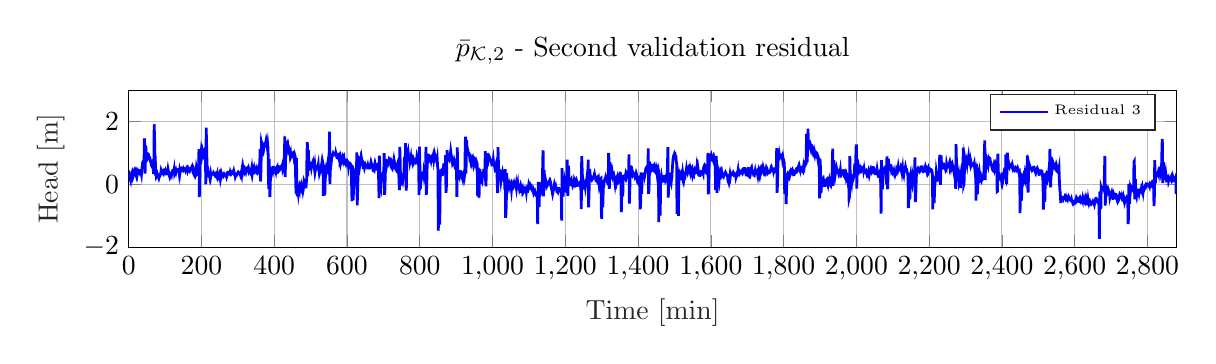
\begin{tikzpicture}

\begin{axis}[%
width=5.239in,
height=0.784in,
at={(0.929in,0.429in)},
scale only axis,
xmin=0,
xmax=2880,
xlabel style={font=\color{white!15!black}},
xlabel={Time [min]},
ymin=-2,
ymax=3,
ylabel style={font=\color{white!15!black}},
ylabel={Head  [m]},
axis background/.style={fill=white},
title style={},
title={$\bar{p}_{\mathcal{K},2}$ - Second validation residual},
xmajorgrids,
ymajorgrids,
legend style={legend cell align=left, align=left, draw=white!15!black}
]
\addplot [color=blue, line width=1.0pt]
  table[row sep=crcr]{%
0	0.449133919282588\\
1	0.344740985305123\\
2	0.281198299437797\\
3	0.217708046706804\\
4	0.174670943788072\\
5	0.131926354608211\\
6	0.251958146202448\\
7	0.331485274233728\\
8	0.329471655834958\\
9	0.359968984163466\\
10	0.398871339937045\\
11	0.356234832343901\\
12	0.252697321895653\\
13	0.291778801833715\\
14	0.371481795574063\\
15	0.410684087336534\\
16	0.360240327865824\\
17	0.367110970025038\\
18	0.406256786507548\\
19	0.355994109843323\\
20	0.310692413844777\\
21	0.27186473673796\\
22	0.348840691615479\\
23	0.301783803729293\\
24	0.37911370886976\\
25	0.378347576502691\\
26	0.430251546038875\\
27	0.408958901389923\\
28	0.448918855627348\\
29	0.448132571770401\\
30	0.406836797616535\\
31	0.397567872336985\\
32	0.356371341649208\\
33	0.372975649708643\\
34	0.392833101768879\\
35	0.331136649202392\\
36	0.465131462287211\\
37	0.566714627925677\\
38	0.688736228662037\\
39	0.725989365666514\\
40	0.725685653568938\\
41	0.684615747124845\\
42	0.594668749676799\\
43	1.47163744137019\\
44	1.31197405058614\\
45	0.347049503957898\\
46	0.787214586629084\\
47	1.2477142284688\\
48	0.876464686377403\\
49	0.886441922562142\\
50	0.89837757768364\\
51	0.868790324145792\\
52	0.935244035322214\\
53	0.976142244320577\\
54	0.969854671062542\\
55	0.880016408890874\\
56	0.863562954109867\\
57	0.86531802733257\\
58	0.860318910391896\\
59	0.763114490768999\\
60	0.727025783341105\\
61	0.725274136474212\\
62	0.615838549527624\\
63	0.595523460153267\\
64	0.620110236051069\\
65	0.740769372328273\\
66	0.761590829709093\\
67	0.767658080729653\\
68	0.335188371455686\\
69	0.476517908100327\\
70	1.920300020265\\
71	1.5126067018042\\
72	0.921316815264674\\
73	0.88057608917206\\
74	0.28952205992762\\
75	0.363068029972986\\
76	0.240963634212626\\
77	0.261654761084799\\
78	0.282344520171719\\
79	0.323194728247039\\
80	0.282920412513676\\
81	0.262806324158369\\
82	0.242690424817219\\
83	0.202173063357996\\
84	0.243251828535733\\
85	0.255582656499165\\
86	0.276257480536565\\
87	0.317329476903694\\
88	0.358398994005277\\
89	0.440027370808636\\
90	0.399731063728368\\
91	0.359194312887126\\
92	0.359453715874906\\
93	0.351363758149645\\
94	0.371778875820482\\
95	0.351629287609548\\
96	0.413074485980083\\
97	0.392918039135353\\
98	0.433956615306187\\
99	0.434192402760942\\
100	0.454823909815438\\
101	0.393853324842823\\
102	0.3736777762835\\
103	0.333098532655065\\
104	0.333314102562035\\
105	0.345578440832462\\
106	0.366184683788603\\
107	0.407185866717342\\
108	0.488981418669432\\
109	0.427975368831618\\
110	0.387363926536395\\
111	0.34674744127166\\
112	0.268534305002127\\
113	0.227907401666968\\
114	0.260526820746939\\
115	0.32188676047619\\
116	0.362841567359112\\
117	0.362991592018496\\
118	0.322336725299742\\
119	0.383673638280328\\
120	0.404205442279249\\
121	0.447993597348542\\
122	0.445043009610487\\
123	0.387070928889656\\
124	0.387089825137913\\
125	0.46526149594149\\
126	0.346090375847012\\
127	0.378561398315981\\
128	0.456970391170174\\
129	0.4773881259704\\
130	0.419415061824161\\
131	0.480631593332348\\
132	0.480649362736315\\
133	0.460267449672102\\
134	0.480684473775909\\
135	0.480701814684025\\
136	0.419520392032965\\
137	0.419537445459298\\
138	0.431607292127687\\
139	0.33797295909131\\
140	0.431402862433316\\
141	0.370458530116963\\
142	0.451835204489882\\
143	0.47225092655011\\
144	0.492666502148417\\
145	0.472282850922568\\
146	0.492698132510498\\
147	0.472314186550271\\
148	0.4927291726801\\
149	0.492744470538369\\
150	0.47236007976359\\
151	0.513174159994435\\
152	0.492789470869752\\
153	0.504857040808588\\
154	0.504871591861559\\
155	0.504885992476474\\
156	0.464101162292806\\
157	0.50491434095013\\
158	0.504928288088216\\
159	0.525341623346989\\
160	0.487763615313369\\
161	0.508176645565285\\
162	0.446991362858839\\
163	0.487803626834591\\
164	0.447017577133259\\
165	0.447030453395726\\
166	0.447043175263019\\
167	0.467455282376349\\
168	0.438721414411845\\
169	0.467479950906785\\
170	0.499944391586872\\
171	0.499956336072344\\
172	0.520367664012454\\
173	0.561178375049394\\
174	0.581351500956984\\
175	0.520402084983402\\
176	0.581373974958098\\
177	0.560985434638631\\
178	0.500035544175333\\
179	0.48261615502787\\
180	0.401028517406026\\
181	0.278640030245498\\
182	0.258487057788905\\
183	0.299056852617802\\
184	0.339864461944195\\
185	0.401071536559861\\
186	0.523477156361658\\
187	0.462286841246495\\
188	0.462295071111306\\
189	0.380705065853078\\
190	0.401112685368794\\
191	0.372374340736606\\
192	0.413181349473902\\
193	1.12717310267643\\
194	-0.404131597496196\\
195	-0.136338728811751\\
196	0.480870005366249\\
197	1.10937624355086\\
198	0.916927332089962\\
199	1.00264388356192\\
200	1.12852390473774\\
201	1.07304695461653\\
202	0.971154206464199\\
203	1.04279492036962\\
204	0.97682937216274\\
205	0.944998901991902\\
206	1.02459201670046\\
207	1.07754696755788\\
208	1.07428023803914\\
209	1.10203174047859\\
210	1.02943596412648\\
211	0.683541617456754\\
212	0.00678191687209306\\
213	1.80993568113976\\
214	1.31512627858028\\
215	0.764344865368301\\
216	0.458357854263205\\
217	0.560361565162957\\
218	0.315573017965583\\
219	0.315578872569105\\
220	0.274785568871614\\
221	0.274791266771203\\
222	0.27479688616603\\
223	0.213841358783803\\
224	0.295207429034186\\
225	0.356411432304\\
226	0.275056128805531\\
227	0.336022422006593\\
228	0.348080913924605\\
229	0.348085980923322\\
230	0.327691428603856\\
231	0.327696336864676\\
232	0.327701165604303\\
233	0.368504994721313\\
234	0.348110124114299\\
235	0.327715173681909\\
236	0.368518763322811\\
237	0.36852319293574\\
238	0.348128002419443\\
239	0.307333191672711\\
240	0.327736920594361\\
241	0.286913588343026\\
242	0.286883492585858\\
243	0.246048542922274\\
244	0.307205589174899\\
245	0.228767918674819\\
246	0.228715148033373\\
247	0.228656884077665\\
248	0.266184577358572\\
249	0.167325539103992\\
250	0.158904958546465\\
251	0.237215887140543\\
252	0.158740763766211\\
253	0.219849650993631\\
254	0.260554003643534\\
255	0.342052513690533\\
256	0.301148933276778\\
257	0.341838734707224\\
258	0.341724750444854\\
259	0.300807053105821\\
260	0.280284335454731\\
261	0.320955750399776\\
262	0.340985611266191\\
263	0.320449651796736\\
264	0.320308964470549\\
265	0.29976454272169\\
266	0.279216000103489\\
267	0.279062950283603\\
268	0.278905927039183\\
269	0.238183515946176\\
270	0.278817846412586\\
271	0.372063129787868\\
272	0.392290492823903\\
273	0.392114712791724\\
274	0.351136324021063\\
275	0.350953560916309\\
276	0.350767417951481\\
277	0.330178429665217\\
278	0.329985750655744\\
279	0.390988535575808\\
280	0.349990539127674\\
281	0.370188156057999\\
282	0.349583761152815\\
283	0.369775589232418\\
284	0.349165555146357\\
285	0.34895235376819\\
286	0.348736519990567\\
287	0.389317208719987\\
288	0.368696794871759\\
289	0.421325742806459\\
290	0.368247899116824\\
291	0.347620487038583\\
292	0.326990892029407\\
293	0.248368252212551\\
294	0.280586747994057\\
295	0.280350594999653\\
296	0.300512098462917\\
297	0.30027225314744\\
298	0.340829753774244\\
299	0.340586515016597\\
300	0.381140771494884\\
301	0.397628345120744\\
302	0.379721700409632\\
303	0.370651590820856\\
304	0.369920751641516\\
305	0.348784853086329\\
306	0.348044631663157\\
307	0.306503115161419\\
308	0.346559181725397\\
309	0.325417678930386\\
310	0.283879302862474\\
311	0.446340597202379\\
312	0.547609132313909\\
313	0.607848466395993\\
314	0.525775134290079\\
315	0.618724138460692\\
316	0.45483770355375\\
317	0.453923633166816\\
318	0.412463098063242\\
319	0.452617268155137\\
320	0.451990355191725\\
321	0.451382869699955\\
322	0.409997140149201\\
323	0.470631332126331\\
324	0.449690947522186\\
325	0.449175023729218\\
326	0.501537391320696\\
327	0.521474760881809\\
328	0.480242288628332\\
329	0.442247597035276\\
330	0.499866276866463\\
331	0.461935198115768\\
332	0.478820704914426\\
333	0.478549100885395\\
334	0.379523328029002\\
335	0.358924699593906\\
336	0.338363870152172\\
337	0.419602043027041\\
338	0.358558137517477\\
339	0.472329187829317\\
340	0.37377615787652\\
341	0.452208354404917\\
342	0.434864163769412\\
343	0.492983983008543\\
344	0.53395676206609\\
345	0.455785523300264\\
346	0.473242439442252\\
347	0.435963070638032\\
348	0.468774673113657\\
349	0.448782149208512\\
350	0.42883796688389\\
351	0.490540754150643\\
352	0.450295078919126\\
353	0.471297648698936\\
354	0.431629868112395\\
355	0.472653929686771\\
356	0.412209131530688\\
357	0.433413259219513\\
358	0.454430937259943\\
359	0.496136648114287\\
360	0.488747764384421\\
361	1.12354761924723\\
362	0.097299979930412\\
363	0.254574389785503\\
364	0.765362381263706\\
365	1.33419942939243\\
366	1.28291657091614\\
367	1.21608940053487\\
368	1.14195223499776\\
369	1.09525083924596\\
370	1.16972299867573\\
371	1.12611021781769\\
372	1.1975059205439\\
373	1.21348626227597\\
374	1.28359784901853\\
375	1.31121636860748\\
376	1.33066042870486\\
377	1.35842029613063\\
378	1.4205946157175\\
379	1.3652572418658\\
380	1.28075364640328\\
381	1.18695825065048\\
382	1.27674610661911\\
383	1.14998386105039\\
384	0.186775873360503\\
385	-0.143053900639593\\
386	0.807321093163033\\
387	0.0384431606819575\\
388	-0.404114432057348\\
389	-0.0391296740339087\\
390	0.395285070267889\\
391	0.339975187772374\\
392	0.468104411863287\\
393	0.453259145282516\\
394	0.519813567119812\\
395	0.537004038960163\\
396	0.541901741390866\\
397	0.468151446207933\\
398	0.530501557850435\\
399	0.526219162705516\\
400	0.451578475195973\\
401	0.475393592411841\\
402	0.43766045763396\\
403	0.440360681551731\\
404	0.40188083336993\\
405	0.505566239883336\\
406	0.519134799673232\\
407	0.540627962411797\\
408	0.483299312673601\\
409	0.521106640407879\\
410	0.434136535477094\\
411	0.41304101736425\\
412	0.432276716620748\\
413	0.442692639045262\\
414	0.448922873140091\\
415	0.560376526650558\\
416	0.557295242469891\\
417	0.533329827917797\\
418	0.56173278862623\\
419	0.57759999838629\\
420	0.572352441785355\\
421	0.545832426007074\\
422	0.591994668428484\\
423	0.506355600742573\\
424	0.556546035115076\\
425	0.522675646380932\\
426	0.574784377038171\\
427	0.504228829877469\\
428	0.983976585160818\\
429	1.53674821635607\\
430	0.232619208336843\\
431	0.670544502541055\\
432	1.27206882087932\\
433	1.23152622020193\\
434	1.26124189703947\\
435	1.1108069260755\\
436	1.1479177655122\\
437	1.15691827826647\\
438	1.20715595104203\\
439	1.11273611572739\\
440	1.15079377126995\\
441	1.09878446950008\\
442	1.12553784930837\\
443	1.11332168810593\\
444	0.947027477141468\\
445	0.994586342536557\\
446	0.88271634313238\\
447	0.908817277674331\\
448	0.906765731286953\\
449	0.956598665520715\\
450	0.99307617708498\\
451	1.00263382469873\\
452	0.950338453860844\\
453	0.886982513064922\\
454	0.876220797495165\\
455	0.791905799264569\\
456	0.821590731734219\\
457	0.914414407793693\\
458	0.872326779615236\\
459	0.0687410371019652\\
460	-0.28732251439461\\
461	0.846759739070862\\
462	0.197561529192264\\
463	-0.381536527144036\\
464	-0.144080159085078\\
465	-0.13556673811825\\
466	-0.243713331324471\\
467	-0.123877994146532\\
468	-0.128792490116943\\
469	-0.0802251082597607\\
470	-0.141864988680965\\
471	-0.022716515361239\\
472	-0.0457262109064658\\
473	-0.0762088219102139\\
474	-0.114900710222472\\
475	-0.0340109841844125\\
476	-0.0830068362520251\\
477	-0.102644056881331\\
478	-0.118469692823595\\
479	-0.203251360511857\\
480	-0.139761568440349\\
481	-0.0387264259408795\\
482	0.111464377808687\\
483	0.0817424618737306\\
484	0.122292569025873\\
485	0.113185305418497\\
486	0.011370825687159\\
487	-0.12269500758903\\
488	0.0491877855021343\\
489	0.114351611653802\\
490	1.02120190459926\\
491	1.3494811508231\\
492	0.262896391839888\\
493	0.692760275889498\\
494	1.09209860788971\\
495	0.727896616009268\\
496	0.664969389198824\\
497	0.671290335055623\\
498	0.618627767330246\\
499	0.66143048306342\\
500	0.644108901683296\\
501	0.612763494125346\\
502	0.534153641142083\\
503	0.599418162098083\\
504	0.641155521472669\\
505	0.584155114378447\\
506	0.597038056447396\\
507	0.62073003064836\\
508	0.686026112128602\\
509	0.630986606142336\\
510	0.557462923891741\\
511	0.460556753522781\\
512	0.570028561350078\\
513	0.450495849155082\\
514	0.516174423719271\\
515	0.519169536640312\\
516	0.531627158395594\\
517	0.537667941412494\\
518	0.583242123242911\\
519	0.584085006078318\\
520	0.562889747468645\\
521	0.627115385722689\\
522	0.469062039263008\\
523	0.430068083238567\\
524	0.338175763027564\\
525	0.379385189746635\\
526	0.424266988257692\\
527	0.420573830287132\\
528	0.546696861822838\\
529	0.5695695474883\\
530	0.617675224092118\\
531	0.687636385622234\\
532	0.768882832883648\\
533	0.711709944492036\\
534	0.66477612638635\\
535	-0.360298205933987\\
536	-0.163384375344386\\
537	0.635341159595633\\
538	0.0796459770365558\\
539	-0.348756711951104\\
540	0.17279030011435\\
541	0.25711432893339\\
542	0.37067767329404\\
543	0.37363072282325\\
544	0.528220391715635\\
545	0.499209788548285\\
546	0.580302875093409\\
547	0.493293856004037\\
548	0.51341567592214\\
549	0.463751850338546\\
550	0.527872925966072\\
551	1.06094277817773\\
552	1.68468672777364\\
553	0.0159339567099366\\
554	0.406272793140317\\
555	0.902432791405715\\
556	0.819909829088132\\
557	0.757061743566474\\
558	0.861422183348566\\
559	0.882469297136737\\
560	0.953603651663371\\
561	0.957288986398837\\
562	0.997929405575675\\
563	0.976365681585868\\
564	0.945582761957731\\
565	0.944025887355281\\
566	0.962143769723653\\
567	0.946141605501097\\
568	0.943038682526179\\
569	1.00744871180829\\
570	0.950720467572651\\
571	0.911397878269298\\
572	0.932255409686277\\
573	0.920660485628929\\
574	0.862632877211958\\
575	0.863092645402524\\
576	0.839822618519783\\
577	0.902921519973916\\
578	0.882359724258102\\
579	0.909086586315226\\
580	0.750075739939604\\
581	0.789218702364764\\
582	0.712748404416971\\
583	0.790974024393933\\
584	0.730988327812774\\
585	0.776166557744055\\
586	0.770514451749712\\
587	0.793159246628903\\
588	0.759967994543565\\
589	0.888539403409752\\
590	0.866529303842846\\
591	0.889329611288268\\
592	0.785567891824194\\
593	0.745227123244035\\
594	0.674250325986378\\
595	0.675530127801672\\
596	0.651958411535993\\
597	0.717455327171891\\
598	0.779637693525046\\
599	0.782338083213375\\
600	0.744725991769812\\
601	0.698372646874923\\
602	0.695379363697519\\
603	0.660324315533401\\
604	0.5792034576777\\
605	0.681185891952971\\
606	0.66595403057481\\
607	0.6847871780828\\
608	0.682185330507657\\
609	0.655032248391784\\
610	0.605030741617384\\
611	0.623905248812143\\
612	0.605928068701722\\
613	-0.310782700358835\\
614	-0.532714525441392\\
615	0.598176880936471\\
616	0.0198136398812068\\
617	-0.497173084622503\\
618	-0.157437776818803\\
619	0.144648233075536\\
620	0.104785134368484\\
621	0.243558442680865\\
622	0.346376209899027\\
623	0.420627214751121\\
624	0.404140798791424\\
625	0.461085706764536\\
626	0.482076127021443\\
627	1.02528831638998\\
628	-0.668137601197188\\
629	-0.310845127809337\\
630	0.164453633605561\\
631	0.779281630119144\\
632	0.676355024249681\\
633	0.816002657228999\\
634	0.794887814420932\\
635	0.812469716865444\\
636	0.678124249285084\\
637	0.757339181965342\\
638	0.676661031043388\\
639	0.711670348541197\\
640	0.815187072167497\\
641	0.737807337724632\\
642	0.75992785420916\\
643	0.732290506272889\\
644	0.724890823731108\\
645	0.495201729091932\\
646	0.59675068656577\\
647	0.595846796564679\\
648	0.530341476257071\\
649	0.574211953483776\\
650	0.611730887619188\\
651	0.569423152537652\\
652	0.580548253295248\\
653	0.578856848020401\\
654	0.580350540441458\\
655	0.557048740054142\\
656	0.576508881397949\\
657	0.616900817109347\\
658	0.557598652334242\\
659	0.55356771449469\\
660	0.536295884984177\\
661	0.52175883929926\\
662	0.522682856304286\\
663	0.619759581114558\\
664	0.623191865232627\\
665	0.661531244968053\\
666	0.719257888824188\\
667	0.676448026570775\\
668	0.636493406676912\\
669	0.577553935135661\\
670	0.536642562490769\\
671	0.493064433471353\\
672	0.511231429090273\\
673	0.488109690379069\\
674	0.532284133457814\\
675	0.570310609214886\\
676	0.628821622474469\\
677	0.55616053990542\\
678	0.611362090978368\\
679	0.553990357852818\\
680	0.526328067835607\\
681	0.51142002203428\\
682	0.531389938200221\\
683	0.568368899448075\\
684	0.536000048876659\\
685	0.498475185362558\\
686	0.550474327962917\\
687	0.123699382489328\\
688	-0.435567147649273\\
689	0.918218613954423\\
690	0.580909296596815\\
691	0.0191853171362339\\
692	-0.0937667979968992\\
693	-0.134219560811147\\
694	0.181187834642728\\
695	0.129390633381306\\
696	0.147127177664245\\
697	0.176907603912404\\
698	0.296624818363071\\
699	0.346791127051354\\
700	0.298163342339372\\
701	0.31563305633702\\
702	0.998177462834924\\
703	-0.327407555016229\\
704	-0.213086095524183\\
705	0.182369621114233\\
706	0.813803741368631\\
707	0.709364254168207\\
708	0.683873341001515\\
709	0.624725571490423\\
710	0.695586825671825\\
711	0.674735684370468\\
712	0.654562466522954\\
713	0.71415534213817\\
714	0.753788024469671\\
715	0.757237106691328\\
716	0.8174199098355\\
717	0.803031702912008\\
718	0.747202530850146\\
719	0.764632335277867\\
720	0.652547005438855\\
721	0.569558094383865\\
722	0.550480792445505\\
723	0.527589830948862\\
724	0.509453073691354\\
725	0.630287584576813\\
726	0.596697826784933\\
727	0.659681409722587\\
728	0.722403779407472\\
729	0.800446605678779\\
730	0.739069185473319\\
731	0.679021760580582\\
732	0.584399539103771\\
733	0.544657060103617\\
734	0.482629954496815\\
735	0.465191528880844\\
736	0.554639805977388\\
737	0.534575354613374\\
738	0.611853626409378\\
739	0.652914740185295\\
740	0.571405103175309\\
741	0.454012632305286\\
742	0.434304186431966\\
743	0.0908392293127562\\
744	-0.177595665125374\\
745	1.19726415147311\\
746	0.820536977050267\\
747	0.240301135891663\\
748	0.0965771975020644\\
749	-0.0321095144822223\\
750	0.244236759794191\\
751	0.202549682473339\\
752	0.152529838617241\\
753	0.110869660312517\\
754	0.203673742103703\\
755	0.20284015993019\\
756	0.286589374868697\\
757	0.542631665340991\\
758	0.880286334149332\\
759	0.797911419423571\\
760	0.759320666653899\\
761	1.32141392474522\\
762	0.0660090150278236\\
763	-0.195726047386792\\
764	0.448925769789128\\
765	1.08262409001776\\
766	1.00136113896027\\
767	0.968539998259317\\
768	1.02900511719976\\
769	0.914843124215977\\
770	0.772817650387267\\
771	0.955262461824731\\
772	0.832760532130152\\
773	0.72164492007186\\
774	0.781130262382092\\
775	0.84175855916741\\
776	0.648025155374071\\
777	0.731591116635471\\
778	0.788631007093947\\
779	0.729459969182891\\
780	0.689141339000393\\
781	0.771159300866614\\
782	0.731586286260615\\
783	0.783847740930028\\
784	0.74430056847666\\
785	0.785716715333976\\
786	0.767768667854611\\
787	0.735191134346024\\
788	0.715032310237419\\
789	0.738028958636889\\
790	0.73853238672055\\
791	0.767846950998155\\
792	0.86911731300242\\
793	0.813998276421614\\
794	0.738979150125914\\
795	0.760509726659393\\
796	0.841902830896984\\
797	0.620177329311531\\
798	-0.334376351122543\\
799	1.20907544530819\\
800	0.776696572521814\\
801	0.238104008042228\\
802	-0.137253220634051\\
803	0.311756224988144\\
804	0.14047280617924\\
805	0.201969651993373\\
806	0.214123662523633\\
807	0.308152490074939\\
808	0.308569280071822\\
809	0.402677271432296\\
810	0.199415197168022\\
811	0.342510587010075\\
812	0.253379015397485\\
813	0.318163566784733\\
814	0.336010341998801\\
815	0.471155689001755\\
816	0.410691635740299\\
817	1.19870165567556\\
818	-0.330023713396848\\
819	-0.0997694832928318\\
820	0.389056978428663\\
821	0.98351507242181\\
822	0.8040243555538\\
823	0.865159429313046\\
824	0.917839820867457\\
825	0.919612168915812\\
826	0.879769093361574\\
827	0.808029500453301\\
828	0.830924964616869\\
829	0.809597323434247\\
830	0.811569828894335\\
831	0.759617321172179\\
832	0.825008182870739\\
833	0.808299131878229\\
834	0.871813698968168\\
835	0.859963592886992\\
836	0.884292471009417\\
837	0.944379091407043\\
838	0.984085916118133\\
839	0.835274749369617\\
840	0.916665260817929\\
841	0.957373770226326\\
842	0.905390963465152\\
843	0.906884088377375\\
844	0.886721709931571\\
845	0.889349092305345\\
846	0.754451091685596\\
847	0.711827205610298\\
848	0.789874890858968\\
849	0.575358429940174\\
850	0.489321386839066\\
851	-1.47469645715744\\
852	-0.632549761267853\\
853	-0.517614327443418\\
854	-0.973958991646434\\
855	-1.27940092249044\\
856	0.22236767106611\\
857	0.283874886277026\\
858	0.439268275575238\\
859	0.451862031716871\\
860	0.411600307941299\\
861	0.374543705221875\\
862	0.27307764677473\\
863	0.408057151230331\\
864	0.420636422094987\\
865	0.538181053287417\\
866	0.518301378746663\\
867	0.673668329663244\\
868	0.572184424488306\\
869	0.491096975653761\\
870	0.328408250392933\\
871	0.932552616702949\\
872	-0.267149008110806\\
873	-0.135627959827431\\
874	0.438900201486376\\
875	1.09092046426927\\
876	0.969837963898868\\
877	0.919211527881899\\
878	0.920675659076736\\
879	0.888112556619731\\
880	0.803408730589489\\
881	0.78395380466489\\
882	0.85307584681005\\
883	0.854289802809816\\
884	0.95456613465079\\
885	1.05535037812219\\
886	0.963547278688765\\
887	0.902527815481534\\
888	0.820167618194191\\
889	0.759681135593844\\
890	0.664538592297255\\
891	0.688240691357898\\
892	0.711342750793037\\
893	0.714967922545078\\
894	0.674407252734433\\
895	0.759563928872829\\
896	0.717022061333303\\
897	0.605764074881407\\
898	0.767117803711216\\
899	0.767321542190537\\
900	0.631520188905405\\
901	0.385411430912974\\
902	-0.396580222365792\\
903	1.17977573517724\\
904	0.762246573766348\\
905	0.303923629841755\\
906	0.151599122766314\\
907	0.415616652822472\\
908	0.312447945442074\\
909	0.270246262135387\\
910	0.362738175311108\\
911	0.381983387827802\\
912	0.413524954652949\\
913	0.412144825273913\\
914	0.402661517591724\\
915	0.340331333797025\\
916	0.232069794234178\\
917	0.210550295944643\\
918	0.168637113993711\\
919	0.281580012447655\\
920	0.300877270561955\\
921	0.311834293387321\\
922	0.371705443589775\\
923	0.292468100505033\\
924	0.389942484141187\\
925	1.31890294526089\\
926	1.52632115905048\\
927	0.343721312185579\\
928	0.896709573387135\\
929	1.41492649485063\\
930	1.06697785007515\\
931	1.04470251864992\\
932	1.08540584442471\\
933	1.0308316273434\\
934	1.00655996038286\\
935	0.995858625344844\\
936	0.934414125682288\\
937	0.909754884507521\\
938	0.785573039114823\\
939	0.792332593570123\\
940	0.731029406430686\\
941	0.790161725426493\\
942	0.737219222212879\\
943	0.857793082507527\\
944	0.857392557841038\\
945	0.875903353771335\\
946	0.803325492811524\\
947	0.741812043419962\\
948	0.735411957804203\\
949	0.622239173509435\\
950	0.661686705860291\\
951	0.720330735246982\\
952	0.782343985917066\\
953	0.760688832267988\\
954	0.724836481746344\\
955	0.643566319193098\\
956	0.720888072393166\\
957	0.68681651693236\\
958	0.644133318764879\\
959	-0.331531157445255\\
960	-0.343173659065535\\
961	0.534389939793513\\
962	-0.00862221856823453\\
963	-0.420658697176975\\
964	0.240370626684502\\
965	0.493411239669229\\
966	0.38808460571223\\
967	0.379861968724718\\
968	0.23422634279472\\
969	0.0888384189221014\\
970	0.0985497908035171\\
971	0.0760581129541293\\
972	0.249229487878154\\
973	0.250847081385039\\
974	0.290306365589089\\
975	0.382868485609578\\
976	0.364837361110148\\
977	0.413653442010286\\
978	0.396117924262974\\
979	0.375619482014223\\
980	1.06076483468597\\
981	0.108789824552588\\
982	-0.059350875995051\\
983	0.487865564133024\\
984	0.996389969807687\\
985	0.777049425634956\\
986	0.755465242066656\\
987	0.792627241891779\\
988	0.755137292415832\\
989	0.835129872475221\\
990	0.874864359040316\\
991	0.833170071619207\\
992	0.850848706506909\\
993	0.817914641897602\\
994	0.777283708553227\\
995	0.775850312486945\\
996	0.760430121789653\\
997	0.69865598894124\\
998	0.719419902364159\\
999	0.637482390618793\\
1000	0.644163606400717\\
1001	0.707277451949686\\
1002	0.786730615170896\\
1003	0.675996978813053\\
1004	0.673922979767639\\
1005	0.612013268045985\\
1006	0.675951871846522\\
1007	0.67506979042011\\
1008	0.581045201536433\\
1009	0.62159704029191\\
1010	0.665793030093617\\
1011	0.584596911494778\\
1012	0.492108809288183\\
1013	0.00512031952902703\\
1014	-0.273210835144631\\
1015	1.18817954865755\\
1016	0.785254128698305\\
1017	0.27220419652776\\
1018	0.431838637984711\\
1019	0.317633762888995\\
1020	0.494612676117107\\
1021	0.253940301385967\\
1022	0.21404231486207\\
1023	0.10458694342006\\
1024	0.186824258770969\\
1025	0.199740770631337\\
1026	0.241390370087842\\
1027	0.277889338007157\\
1028	0.360312628826499\\
1029	0.299926421255037\\
1030	0.373977903746145\\
1031	0.377736341220398\\
1032	0.329364997447179\\
1033	0.248528218177597\\
1034	-0.179113536345014\\
1035	0.486460564206929\\
1036	-1.06125368917119\\
1037	-0.924510715660624\\
1038	-0.495717521652097\\
1039	0.360506733187734\\
1040	0.0753892826956886\\
1041	0.0217315967136145\\
1042	0.0643627577067818\\
1043	0.0438005532783379\\
1044	-0.0177461589984489\\
1045	-0.0773891605499202\\
1046	-0.0156812226399765\\
1047	-0.0754036001977028\\
1048	-0.0548531055106807\\
1049	0.0253794645070116\\
1050	0.0466843214445234\\
1051	-0.0661085342155445\\
1052	-0.164917314006352\\
1053	-0.0412856361266236\\
1054	-0.0601743758324815\\
1055	-0.039982860121313\\
1056	0.000851563677997547\\
1057	-0.0395634432790857\\
1058	0.00272301823434162\\
1059	0.0436074641086961\\
1060	-0.00981732372276412\\
1061	-0.00803985201029178\\
1062	-0.00908464907051609\\
1063	-0.0480627223087495\\
1064	-0.0879418660130895\\
1065	-0.00596609415065075\\
1066	-0.107109656090209\\
1067	-0.0259315905383417\\
1068	-0.0368578610764629\\
1069	0.0216078671510829\\
1070	-0.158139765581737\\
1071	-0.0179232088584911\\
1072	-0.0373103854403141\\
1073	-0.0566754890875529\\
1074	-0.138867877438038\\
1075	-0.0972822667481594\\
1076	-0.230231138445895\\
1077	-0.230954673983028\\
1078	-0.229168795110503\\
1079	-0.130732060297255\\
1080	-0.187614445581112\\
1081	-0.188847709673091\\
1082	-0.151702953395883\\
1083	-0.286163586108572\\
1084	-0.268460418486612\\
1085	-0.195797226620833\\
1086	-0.230474178017353\\
1087	-0.210875134552644\\
1088	-0.149904852577031\\
1089	-0.172433685205824\\
1090	-0.193279192084539\\
1091	-0.116230018440575\\
1092	-0.116721149074792\\
1093	-0.219793083470385\\
1094	-0.119187031527183\\
1095	-0.138200021405765\\
1096	-0.131138998884502\\
1097	-0.153009694082634\\
1098	-0.113270669112012\\
1099	-0.0366205891462457\\
1100	-0.0941811983612055\\
1101	-0.0544625803771055\\
1102	-0.0559787434947481\\
1103	-0.0154510274028112\\
1104	-0.0481350072508064\\
1105	-0.0119719351337864\\
1106	-0.0126059740975322\\
1107	-0.094292775718138\\
1108	-0.137009897858114\\
1109	-0.15810250652293\\
1110	-0.199858353264268\\
1111	-0.200134681183712\\
1112	-0.241246551766871\\
1113	-0.181633827781788\\
1114	-0.213851736614494\\
1115	-0.214685695726352\\
1116	-0.196103364796052\\
1117	-0.236988479029414\\
1118	-0.319085458862006\\
1119	-0.339709250485754\\
1120	-0.352875669308624\\
1121	-0.332241986833772\\
1122	-0.353535788703702\\
1123	-0.414765721722326\\
1124	-1.26633251341059\\
1125	-0.372251019255401\\
1126	0.0829788339777693\\
1127	-0.315567597253001\\
1128	-0.714107296615275\\
1129	-0.26791230807661\\
1130	-0.37763434735119\\
1131	-0.0572643847409466\\
1132	-0.0445705621996453\\
1133	-0.0146752187806527\\
1134	-0.0663669807185201\\
1135	-0.13010020171734\\
1136	-0.0800067376746583\\
1137	-0.160905510767414\\
1138	0.815777357066324\\
1139	1.09024308081315\\
1140	-0.378255347223188\\
1141	0.0292704785464579\\
1142	0.458555676288597\\
1143	0.0104793967226087\\
1144	-0.00098939867447001\\
1145	0.000324028902511486\\
1146	-0.0190953111153149\\
1147	0.0628620982604886\\
1148	0.00267546132203478\\
1149	-0.0695886141842479\\
1150	-0.0481929990575338\\
1151	0.0108541502810766\\
1152	0.0119482590995332\\
1153	0.0130879786984579\\
1154	0.0550709973931163\\
1155	0.0358859652596166\\
1156	0.0454918797857147\\
1157	0.0876038561575285\\
1158	0.0481431837351778\\
1159	0.0903220287856144\\
1160	0.0512618234634132\\
1161	-0.0613933316293682\\
1162	-0.141444169996127\\
1163	-0.160312387971501\\
1164	-0.240168718284167\\
1165	-0.299912915954401\\
1166	-0.237029828556587\\
1167	-0.194528118227709\\
1168	-0.151751449826428\\
1169	-0.0838315615621852\\
1170	-0.00868433072928809\\
1171	-0.0597124768493131\\
1172	-0.057793550255731\\
1173	-0.0354320333238789\\
1174	-0.114779104641293\\
1175	-0.112970432796359\\
1176	-0.163747494171034\\
1177	-0.222451393548994\\
1178	-0.220396030957318\\
1179	-0.238509490032428\\
1180	-0.154657478225296\\
1181	-0.126908660915412\\
1182	-0.124601849686982\\
1183	-0.163047494699079\\
1184	-0.160618711367597\\
1185	-0.178603357439279\\
1186	-0.216684663322177\\
1187	-0.22940831185538\\
1188	-0.206454144128145\\
1189	-0.346669213129076\\
1190	-1.15212797104417\\
1191	0.522076367573661\\
1192	0.229754779556366\\
1193	-0.135895311367399\\
1194	-0.387184261222764\\
1195	0.0347841755142539\\
1196	-0.16400669138001\\
1197	-0.0274879147022702\\
1198	0.0680661094021175\\
1199	-0.0285133449003894\\
1200	-0.0753782889479453\\
1201	-0.114829209604757\\
1202	-0.215455306712784\\
1203	-0.219435467427374\\
1204	-0.177218264815984\\
1205	0.795054578486614\\
1206	0.234157291816587\\
1207	-0.358325034330832\\
1208	0.130492266499793\\
1209	0.601543258545625\\
1210	0.122152948122739\\
1211	0.0627819396131954\\
1212	0.105482374527867\\
1213	0.112355893659554\\
1214	0.114257667370602\\
1215	0.136613632684302\\
1216	0.158796900699699\\
1217	0.00618609873270515\\
1218	0.00808883887203393\\
1219	-0.0103310334159872\\
1220	-0.0439612827616287\\
1221	-0.00111376977417166\\
1222	0.0619843126162252\\
1223	0.0437407236843725\\
1224	0.0220896568873954\\
1225	0.147166393526554\\
1226	0.115989670512825\\
1227	0.118060815098843\\
1228	0.0797104432104376\\
1229	0.142532516525264\\
1230	0.162494739928846\\
1231	0.12318486759041\\
1232	0.0927617474816671\\
1233	0.0745878159452431\\
1234	-0.0256316019911011\\
1235	-0.0232268704085854\\
1236	-0.000309597669023276\\
1237	-0.00993029118763644\\
1238	0.0326965332792426\\
1239	0.0348096438079466\\
1240	0.0542806013453827\\
1241	0.0352721311308457\\
1242	-0.0726593052560034\\
1243	-0.217532437338683\\
1244	-0.783165904337267\\
1245	0.90103841933032\\
1246	0.617725744635898\\
1247	0.224045498491392\\
1248	-0.0388768298873856\\
1249	0.126605827376736\\
1250	0.038962551035624\\
1251	0.000478353266061049\\
1252	-0.0635292115377908\\
1253	-0.0439954501592936\\
1254	-0.00918655380262834\\
1255	-0.0852076004586451\\
1256	0.0108258365238854\\
1257	0.0132202307740528\\
1258	0.150077624017797\\
1259	0.172658946197132\\
1260	0.268741068859853\\
1261	0.208239195406975\\
1262	0.229336364796296\\
1263	0.792875732226108\\
1264	-0.732162096017291\\
1265	-0.401951124893863\\
1266	0.0464209394881578\\
1267	0.496091256361304\\
1268	0.333440758851829\\
1269	0.28123122752401\\
1270	0.1796912851675\\
1271	0.180904636597958\\
1272	0.239341906362633\\
1273	0.228283562276751\\
1274	0.167378062516512\\
1275	0.188180668314018\\
1276	0.189658699242393\\
1277	0.20910540738614\\
1278	0.218678627685932\\
1279	0.301633586938799\\
1280	0.339477466690283\\
1281	0.266870329756038\\
1282	0.227061825947168\\
1283	0.20710846023136\\
1284	0.146506610572494\\
1285	0.155256695469582\\
1286	0.13313109013945\\
1287	0.235593269459947\\
1288	0.236478425000008\\
1289	0.245968942806705\\
1290	0.204421636592507\\
1291	0.226758302805514\\
1292	0.125207504493694\\
1293	0.0084384345419366\\
1294	0.072371027508936\\
1295	0.113893869563363\\
1296	0.113466003122632\\
1297	0.192211024379098\\
1298	0.201269820417991\\
1299	-0.816546746950678\\
1300	-1.09293792810678\\
1301	0.145882314353194\\
1302	-0.330924863816371\\
1303	-0.726133322151128\\
1304	-0.297013789212365\\
1305	0.0097091206825084\\
1306	0.0020937035780122\\
1307	0.0964765206453748\\
1308	0.138007223457642\\
1309	0.179538517736205\\
1310	0.175133735796706\\
1311	0.228482866447798\\
1312	0.18841773470777\\
1313	0.148353168833665\\
1314	0.120579405780234\\
1315	0.202676370412988\\
1316	0.215465894468018\\
1317	0.257001687839342\\
1318	0.220148173290333\\
1319	1.00812174680777\\
1320	0.795528663879033\\
1321	-0.140821002113711\\
1322	0.240674083879313\\
1323	0.71066960668427\\
1324	0.385434117194166\\
1325	0.364177131042915\\
1326	0.312692382932426\\
1327	0.353383717353374\\
1328	0.31477168192805\\
1329	0.393167705803741\\
1330	0.322380186079229\\
1331	0.386263339711611\\
1332	0.386445519269351\\
1333	0.314414873746038\\
1334	0.233552798156175\\
1335	0.18864886361105\\
1336	0.0897030391910718\\
1337	0.000463420801665393\\
1338	0.0827187885514604\\
1339	0.124272993702419\\
1340	0.0729472667779518\\
1341	0.156936081092773\\
1342	0.195331087521069\\
1343	0.0532062214505231\\
1344	0.0419198998973016\\
1345	0.0646667965495595\\
1346	0.0835392334216891\\
1347	0.186586527555399\\
1348	0.291003756934458\\
1349	0.32095139017737\\
1350	0.303767441949582\\
1351	0.402504039935231\\
1352	0.248578243672974\\
1353	0.107832842348046\\
1354	-0.884514737023949\\
1355	-0.372560066886905\\
1356	0.305808314132591\\
1357	-0.088558626763934\\
1358	-0.380927804199608\\
1359	0.171429983438614\\
1360	0.234198816849165\\
1361	0.268222224479999\\
1362	0.269792254469579\\
1363	0.283415735636055\\
1364	0.284985321983747\\
1365	0.245755508925321\\
1366	0.320576578786955\\
1367	0.395397125767694\\
1368	0.376565504484141\\
1369	0.299743265784727\\
1370	0.35416245908479\\
1371	0.355491774164165\\
1372	0.328311247713394\\
1373	0.370674696284716\\
1374	0.372238161222711\\
1375	0.957041049187346\\
1376	-0.612822457426411\\
1377	-0.272388489910313\\
1378	0.155191584732854\\
1379	0.607733658367444\\
1380	0.494831408521243\\
1381	0.519611472163305\\
1382	0.524818483056826\\
1383	0.416426745482262\\
1384	0.437724641536938\\
1385	0.399241796585983\\
1386	0.312001806918232\\
1387	0.334228000886228\\
1388	0.340581845092267\\
1389	0.304472474076427\\
1390	0.29257865359272\\
1391	0.296119023628414\\
1392	0.23893286032456\\
1393	0.264900094309525\\
1394	0.295264279027769\\
1395	0.359795126471298\\
1396	0.323982247632642\\
1397	0.19345480448235\\
1398	0.134858109555971\\
1399	0.0571834940364511\\
1400	0.0402022317221977\\
1401	0.0924582891156049\\
1402	0.178349708892071\\
1403	0.224838531357236\\
1404	0.235580091650881\\
1405	0.13788718367266\\
1406	-0.79284600625531\\
1407	-0.620557697613485\\
1408	0.386746173318585\\
1409	-0.00521454502391094\\
1410	-0.307314946730486\\
1411	0.198135227248216\\
1412	0.303853381281712\\
1413	0.299139367364759\\
1414	0.335134113194904\\
1415	0.338583902524626\\
1416	0.321540852292372\\
1417	0.33685612511001\\
1418	0.261632178556894\\
1419	0.317552783790681\\
1420	0.381483981757086\\
1421	0.498404284466361\\
1422	0.52157184143288\\
1423	0.54463705406647\\
1424	0.559252590781099\\
1425	0.520911336368847\\
1426	0.482464695645703\\
1427	0.464311309671693\\
1428	1.15168834662597\\
1429	-0.297332243576811\\
1430	-0.183408715083267\\
1431	0.26572635626529\\
1432	0.735248057412079\\
1433	0.522633576153595\\
1434	0.563073756011676\\
1435	0.587080664106125\\
1436	0.554893391776595\\
1437	0.536366539382271\\
1438	0.494953829859831\\
1439	0.525030452462936\\
1440	0.528860628363169\\
1441	0.586437924426626\\
1442	0.578093899239072\\
1443	0.596102789208693\\
1444	0.438993487685941\\
1445	0.421304508687562\\
1446	0.419118206190099\\
1447	0.416015960582904\\
1448	0.397098283903475\\
1449	0.444709199506811\\
1450	0.51860160726708\\
1451	0.46794538502774\\
1452	0.369772834982292\\
1453	0.485300753553162\\
1454	0.459561273944125\\
1455	0.50908750207423\\
1456	0.453949131478701\\
1457	-1.19922765000664\\
1458	0.120588694853531\\
1459	-0.204539328549508\\
1460	-0.631668624422559\\
1461	-0.989500066654749\\
1462	0.275846301258319\\
1463	0.203248075832114\\
1464	0.273333161626169\\
1465	0.195414342129425\\
1466	0.143007471756043\\
1467	0.126279289283147\\
1468	0.155311071798209\\
1469	0.143882295353201\\
1470	0.205846749570959\\
1471	0.255937960670003\\
1472	0.257100756998199\\
1473	0.249433173077747\\
1474	0.239080816387947\\
1475	0.167846855068007\\
1476	0.210772193548493\\
1477	0.181056267161814\\
1478	0.166998143442086\\
1479	0.138098315664422\\
1480	0.109636545905744\\
1481	0.708875806960755\\
1482	1.19132500423933\\
1483	-0.414962100289245\\
1484	-0.0828138919145971\\
1485	0.375583773391647\\
1486	0.158635471676291\\
1487	0.117767810488076\\
1488	0.128577291626875\\
1489	0.0964165466459832\\
1490	0.108802559776812\\
1491	0.0632803351193445\\
1492	0.175685753512013\\
1493	0.257106623967353\\
1494	0.470848389240082\\
1495	0.63534388856138\\
1496	0.80748834081983\\
1497	0.880882940754816\\
1498	0.922351371646009\\
1499	0.922808789593802\\
1500	0.967073205958059\\
1501	0.933367655220827\\
1502	0.949505238957684\\
1503	0.897071255253991\\
1504	0.893347145792418\\
1505	0.737385215181405\\
1506	0.674087484716509\\
1507	-0.93422210908048\\
1508	0.0880423985335597\\
1509	-0.0968485310997025\\
1510	-0.62697507295114\\
1511	-1.00224924781491\\
1512	0.0416005690390548\\
1513	0.161058273563825\\
1514	0.327731880546935\\
1515	0.287204539558772\\
1516	0.287478074482372\\
1517	0.320206161311425\\
1518	0.238884871694566\\
1519	0.218763741266578\\
1520	0.297434348886668\\
1521	0.260123912286524\\
1522	0.211261031554571\\
1523	0.351134101529119\\
1524	0.27302815350501\\
1525	0.249707027105359\\
1526	0.171603018598987\\
1527	0.253488763591307\\
1528	0.270969238659731\\
1529	0.254066093228857\\
1530	0.37675289886505\\
1531	0.397442485216629\\
1532	0.409786082087287\\
1533	0.491437059668542\\
1534	0.41036776419898\\
1535	0.430820445388726\\
1536	0.390550378775984\\
1537	0.452040024871522\\
1538	0.525344676360916\\
1539	0.546034835431364\\
1540	0.505763965808612\\
1541	0.444855193026413\\
1542	0.424507038973559\\
1543	0.384234597481282\\
1544	0.506681889689631\\
1545	0.466169994454731\\
1546	0.486855821021202\\
1547	0.499194134841176\\
1548	0.519877883812214\\
1549	0.356964593417658\\
1550	0.275648189632932\\
1551	0.316727658295861\\
1552	0.317006585114392\\
1553	0.296884415674342\\
1554	0.394018531056282\\
1555	0.45549112349314\\
1556	0.493355052057495\\
1557	0.473225710949187\\
1558	0.435902080569122\\
1559	0.412561304090325\\
1560	0.436431945845811\\
1561	0.436538596025827\\
1562	0.576234354051948\\
1563	0.515141585910705\\
1564	0.576445647533831\\
1565	0.489813124191166\\
1566	0.408319563065106\\
1567	0.326825570190216\\
1568	0.326929298392521\\
1569	0.28623350049719\\
1570	0.286336329328591\\
1571	0.32723777771043\\
1572	0.327339678465925\\
1573	0.388639724417757\\
1574	0.421193017226891\\
1575	0.421293471908761\\
1576	0.421393430254078\\
1577	0.421492885084781\\
1578	0.380792749222849\\
1579	0.343299293034384\\
1580	0.523547809234927\\
1581	0.564444257592157\\
1582	0.605340166549439\\
1583	0.625835988930632\\
1584	0.605532177560193\\
1585	0.524029185263416\\
1586	0.462925164866441\\
1587	0.425427301917857\\
1588	0.364322123208936\\
1589	0.356068173698148\\
1590	0.3765599684695\\
1591	0.417450699290725\\
1592	1.00912839899541\\
1593	-0.315167055454715\\
1594	-0.160249406113294\\
1595	0.413439359546736\\
1596	0.924907289588745\\
1597	0.820570884044045\\
1598	0.86792524171473\\
1599	0.84752983200724\\
1600	0.896655360747651\\
1601	0.934084818154481\\
1602	0.884267928493152\\
1603	0.829418571422096\\
1604	0.844596660033361\\
1605	0.811433249722363\\
1606	0.781625243149414\\
1607	0.833948445484303\\
1608	0.782279429907142\\
1609	0.839861142957403\\
1610	0.789056529542471\\
1611	0.769070156409562\\
1612	0.698182387355999\\
1613	-0.175231055179523\\
1614	-0.0385036656143214\\
1615	0.913251418326283\\
1616	0.342138533840753\\
1617	-0.26977422017098\\
1618	0.0362915291986852\\
1619	0.138361074861628\\
1620	0.0772334897339633\\
1621	0.118143517353985\\
1622	0.261049206970597\\
1623	0.179795624239581\\
1624	0.3549123137728\\
1625	0.334615408089284\\
1626	0.395914517052994\\
1627	0.355213753902149\\
1628	0.396108951907074\\
1629	0.335004224371161\\
1630	0.375894944631767\\
1631	0.294386146061072\\
1632	0.314872742067038\\
1633	0.314957466094299\\
1634	0.274240751625008\\
1635	0.25392119217981\\
1636	0.294797841318683\\
1637	0.327325791948859\\
1638	0.347797998988888\\
1639	0.36826771553887\\
1640	0.38873491532506\\
1641	0.348000952117545\\
1642	0.348063499731047\\
1643	0.307324372025846\\
1644	0.286982162908657\\
1645	0.287036846333493\\
1646	0.246289776302554\\
1647	0.123941846867048\\
1648	0.0831893521281373\\
1649	0.0832331862377345\\
1650	0.0424751633993878\\
1651	0.0985731999232655\\
1652	0.258597453382194\\
1653	0.340228185353737\\
1654	0.282266748261982\\
1655	0.360684204973737\\
1656	0.340308521628145\\
1657	0.319929882278238\\
1658	0.319947801571409\\
1659	0.360761794214362\\
1660	0.360773674973913\\
1661	0.340382958677807\\
1662	0.381187780215619\\
1663	0.360790874539497\\
1664	0.340390836665058\\
1665	0.299588101672157\\
1666	0.28238920764246\\
1667	0.279171680976624\\
1668	0.299557945762373\\
1669	0.221150735538885\\
1670	0.261930002864176\\
1671	0.314759104339281\\
1672	0.335132196657632\\
1673	0.335102394912482\\
1674	0.375868294798522\\
1675	0.45422239445238\\
1676	0.355392162605263\\
1677	0.375748242280054\\
1678	0.355301767095781\\
1679	0.416212113837986\\
1680	0.395758616663223\\
1681	0.375420563436066\\
1682	0.375477306270838\\
1683	0.395928882380517\\
1684	0.355177169115407\\
1685	0.35521990396159\\
1686	0.375657584539248\\
1687	0.355291628601023\\
1688	0.387773305094044\\
1689	0.489795589995921\\
1690	0.489815732419501\\
1691	0.510231010630648\\
1692	0.510242383019367\\
1693	0.510249428098085\\
1694	0.428654024499934\\
1695	0.428652530977068\\
1696	0.36744820639894\\
1697	0.306239709750585\\
1698	0.306225700130895\\
1699	0.367406216750879\\
1700	0.36738405893189\\
1701	0.448956046103945\\
1702	0.510124517803909\\
1703	0.510090433673753\\
1704	0.285657513458794\\
1705	0.285615677005879\\
1706	0.24477094426166\\
1707	0.236374980007028\\
1708	0.277120895033455\\
1709	0.460659894190989\\
1710	0.501398457807426\\
1711	0.521733866301346\\
1712	0.545273129959654\\
1713	0.46360373064222\\
1714	0.443129457990324\\
1715	0.422651732767399\\
1716	0.381771055818476\\
1717	0.34088700806835\\
1718	0.361198250519742\\
1719	0.340707124251423\\
1720	0.32021275041636\\
1721	0.381313330239813\\
1722	0.442410745017533\\
1723	0.38110779611381\\
1724	0.40139992495962\\
1725	0.360490393050746\\
1726	0.360376941945844\\
1727	0.380422202139144\\
1728	0.351556737939234\\
1729	0.290473789533337\\
1730	0.392108590352123\\
1731	0.371581229860837\\
1732	0.330651580748636\\
1733	0.493714624961051\\
1734	0.47317914449124\\
1735	0.473040581377951\\
1736	0.350740059978406\\
1737	0.411794996849665\\
1738	0.350450197441504\\
1739	0.370701103955888\\
1740	0.390949598630776\\
1741	0.51267340296895\\
1742	0.491820422261654\\
1743	0.471188388093687\\
1744	0.552062415248344\\
1745	0.510762073963448\\
1746	0.464308460395301\\
1747	0.422981059039088\\
1748	0.300043411578258\\
1749	0.299491881367217\\
1750	0.360128810942129\\
1751	0.400357001657341\\
1752	0.460976493321482\\
1753	0.541988243833302\\
1754	0.520995968817395\\
1755	0.459199241259988\\
1756	0.417797631144865\\
1757	0.376392545089693\\
1758	0.396183545982851\\
1759	0.375173872620749\\
1760	0.374563079346132\\
1761	0.373952555687069\\
1762	0.405795587578396\\
1763	0.425587911617392\\
1764	0.445383261392848\\
1765	0.505981623589086\\
1766	0.484986658290381\\
1767	0.525196038628643\\
1768	0.483813870433188\\
1769	0.483238271882435\\
1770	0.502832759458684\\
1771	0.502274746929238\\
1772	0.440765993871452\\
1773	0.501189790630328\\
1774	0.500664525784401\\
1775	0.500151839831531\\
1776	0.438691713698312\\
1777	0.458368374575059\\
1778	0.461105736672913\\
1779	0.481050956777075\\
1780	0.492665958131219\\
1781	1.16222283801918\\
1782	-0.263734401149371\\
1783	-0.0582989195676333\\
1784	0.362678596340636\\
1785	0.996809610988784\\
1786	0.905692114348909\\
1787	0.887352131236568\\
1788	0.968633384808371\\
1789	0.896258350664972\\
1790	0.874806125069298\\
1791	0.902347958904983\\
1792	0.904148401391069\\
1793	0.89797492577506\\
1794	0.917291045330408\\
1795	0.908198009190073\\
1796	0.930314873661175\\
1797	0.819294540703581\\
1798	0.878317196201138\\
1799	0.808979172977722\\
1800	0.724672840456833\\
1801	0.734927263963925\\
1802	0.681083197835214\\
1803	-0.300245488476449\\
1804	-0.101200361429655\\
1805	0.373370839787718\\
1806	-0.196668391899244\\
1807	-0.626918452506104\\
1808	-0.193768760147371\\
1809	0.0648351020075353\\
1810	0.22999313473904\\
1811	0.272960125441692\\
1812	0.33653260797238\\
1813	0.318711960814561\\
1814	0.30109474747676\\
1815	0.263279158477943\\
1816	0.31931336807137\\
1817	0.281890632498929\\
1818	0.326256418703338\\
1819	0.330008576886129\\
1820	0.354340177987318\\
1821	0.448889171155486\\
1822	0.435970686316274\\
1823	0.440166001750995\\
1824	0.462177947834661\\
1825	0.408677651926091\\
1826	0.352576740975962\\
1827	0.316762763142322\\
1828	0.321862051933856\\
1829	0.318718732110341\\
1830	0.384975905484026\\
1831	0.36995277345396\\
1832	0.375398279131353\\
1833	0.381324875405653\\
1834	0.439299468055111\\
1835	0.485676238771227\\
1836	0.511671418768771\\
1837	0.517271493273\\
1838	0.46487222634952\\
1839	0.490839304908121\\
1840	0.537168575656494\\
1841	0.575512855541703\\
1842	0.539713656682032\\
1843	0.585845173880067\\
1844	0.529884301250988\\
1845	0.514613422516568\\
1846	0.458420027492622\\
1847	0.51613987867573\\
1848	0.500456007893419\\
1849	0.545568339544523\\
1850	0.549938499741288\\
1851	0.492916779249093\\
1852	0.427342130065639\\
1853	0.41069325964429\\
1854	0.495809727574546\\
1855	0.379894900332204\\
1856	0.505309035309104\\
1857	0.630454909292339\\
1858	0.665376881449461\\
1859	0.647156616962313\\
1860	0.689834856810492\\
1861	0.650931261213557\\
1862	0.672751923618101\\
1863	1.60347983406338\\
1864	1.43549946892872\\
1865	0.711497537355605\\
1866	1.24639845240568\\
1867	1.7767460895874\\
1868	1.41377669466753\\
1869	1.36741766262887\\
1870	1.30561215957404\\
1871	1.26929546149193\\
1872	1.24601835958352\\
1873	1.17996380999413\\
1874	1.1424344518835\\
1875	1.21670770158637\\
1876	1.16988821013263\\
1877	1.14703455481073\\
1878	1.16648062127867\\
1879	1.09749174545831\\
1880	1.13726031467918\\
1881	1.14708704767062\\
1882	1.05787850901969\\
1883	1.09344110343765\\
1884	1.00945285578463\\
1885	1.03768688565329\\
1886	0.968817670002537\\
1887	1.04231608497822\\
1888	1.04075849401387\\
1889	1.02582040244002\\
1890	1.01427136969786\\
1891	0.962309399111511\\
1892	0.910530846110021\\
1893	0.84834163224275\\
1894	0.836633638015236\\
1895	0.761439123417823\\
1896	0.840044593148491\\
1897	0.805448047112321\\
1898	0.631035939320817\\
1899	-0.446089565906142\\
1900	0.822818830752368\\
1901	0.647577375433436\\
1902	0.197473167331829\\
1903	-0.276630275292845\\
1904	0.12145114970852\\
1905	-0.0222387037119489\\
1906	0.0291910785422758\\
1907	0.0166822549306858\\
1908	0.167398840748874\\
1909	0.187901656074629\\
1910	0.0978851114514754\\
1911	0.0662073399519656\\
1912	0.0174806839648767\\
1913	-0.0338184207723415\\
1914	-0.0318388044705884\\
1915	0.060298282068679\\
1916	0.11234220641785\\
1917	0.106887755046166\\
1918	0.151350048375647\\
1919	0.164121013466136\\
1920	0.0582461649179322\\
1921	0.0246167465911213\\
1922	-0.020758070183156\\
1923	0.0512049675397321\\
1924	0.0472583575656955\\
1925	0.104594778438319\\
1926	0.00250278357357558\\
1927	-0.000475922230563697\\
1928	0.0494892178944752\\
1929	-0.0108234786964232\\
1930	-0.0332177576318031\\
1931	0.0211783867270015\\
1932	0.0604047288409078\\
1933	0.100194260679856\\
1934	0.75526992774445\\
1935	1.14086864606336\\
1936	-0.0413416293746707\\
1937	0.359426558304698\\
1938	0.769123162748052\\
1939	0.661160582158381\\
1940	0.46835677346936\\
1941	0.405689340080535\\
1942	0.321319161402933\\
1943	0.401382630474863\\
1944	0.391735926643072\\
1945	0.412540145025979\\
1946	0.495200988957329\\
1947	0.440349283076564\\
1948	0.439794499446542\\
1949	0.418922094901795\\
1950	0.40029982397251\\
1951	0.358348368921831\\
1952	0.409221312394706\\
1953	0.393357888328076\\
1954	0.379718765348905\\
1955	0.385029475331983\\
1956	0.46245061592888\\
1957	0.347329438237672\\
1958	0.368679361026224\\
1959	0.319265708823465\\
1960	0.341823635306191\\
1961	0.384018249349104\\
1962	0.40766207038763\\
1963	0.430529356883959\\
1964	0.44273813469043\\
1965	0.439580601218999\\
1966	0.34660903457484\\
1967	0.369344876924991\\
1968	0.316835256992555\\
1969	0.356649492291659\\
1970	0.306007156533468\\
1971	0.333838043490132\\
1972	0.236748723063094\\
1973	0.282134847670868\\
1974	0.266126630497887\\
1975	0.250428716708775\\
1976	0.16340550497047\\
1977	0.237944927974674\\
1978	0.211028352089613\\
1979	0.217310139592271\\
1980	-0.452792671794214\\
1981	-0.405477615241445\\
1982	0.907260257852144\\
1983	0.373637601399629\\
1984	-0.0752212788427826\\
1985	0.288412288694268\\
1986	0.130195245430897\\
1987	0.0565046509077263\\
1988	0.195844061816885\\
1989	0.162861016209206\\
1990	0.118512151547293\\
1991	0.146870330510865\\
1992	0.224824431891989\\
1993	0.27004196161716\\
1994	0.371508500878043\\
1995	0.551315446222503\\
1996	0.5354242923447\\
1997	0.600845655438313\\
1998	0.567664315859709\\
1999	1.13462715999387\\
2000	1.27917719659408\\
2001	-0.132993416535427\\
2002	0.276836968700749\\
2003	0.77783892946681\\
2004	0.602709774452684\\
2005	0.641197037533288\\
2006	0.57918294757544\\
2007	0.540716078006938\\
2008	0.478473841654655\\
2009	0.522396726611284\\
2010	0.499978985019467\\
2011	0.524790610670927\\
2012	0.467705089518013\\
2013	0.488817610129864\\
2014	0.449782131860438\\
2015	0.47163396927558\\
2016	0.497481642583566\\
2017	0.520705198990917\\
2018	0.546942092123963\\
2019	0.549013054216751\\
2020	0.451038366931364\\
2021	0.508320837655226\\
2022	0.42899415324711\\
2023	0.411469493501308\\
2024	0.39823702445328\\
2025	0.421291092433201\\
2026	0.404650968956453\\
2027	0.423590078708216\\
2028	0.363562070747783\\
2029	0.319782582284098\\
2030	0.348738891605045\\
2031	0.336880641883759\\
2032	0.255706476287124\\
2033	0.256943865972424\\
2034	0.355392810836371\\
2035	0.298388938799867\\
2036	0.362984045937942\\
2037	0.424928480212877\\
2038	0.484482724097951\\
2039	0.508318423532934\\
2040	0.456242517474266\\
2041	0.433613277627998\\
2042	0.455003584918714\\
2043	0.395905580098088\\
2044	0.414619371355251\\
2045	0.543105373590393\\
2046	0.546234919074756\\
2047	0.537485245939934\\
2048	0.527064719405615\\
2049	0.464759478992832\\
2050	0.365426207379159\\
2051	0.344221938260688\\
2052	0.34128386498444\\
2053	0.340253793528277\\
2054	0.361755085228104\\
2055	0.382205886750604\\
2056	0.40455133791847\\
2057	0.485715545193514\\
2058	0.412006663546684\\
2059	0.330508581251941\\
2060	0.288499743574725\\
2061	0.250984596139858\\
2062	0.251646179104078\\
2063	0.314607935279135\\
2064	0.352881278638087\\
2065	0.281370938177133\\
2066	0.40261775932585\\
2067	-0.0825383017361503\\
2068	-0.926899318663303\\
2069	0.772741833864245\\
2070	0.465520028033289\\
2071	0.028173225122984\\
2072	-0.153077067881597\\
2073	0.409122151803189\\
2074	0.481480149061014\\
2075	0.463616282446267\\
2076	0.495381263744811\\
2077	0.515077845143196\\
2078	0.529384649672735\\
2079	0.508252376956264\\
2080	0.478759054679067\\
2081	0.33840848698334\\
2082	0.410646976848902\\
2083	0.328021227850975\\
2084	0.893265143975462\\
2085	0.0487485447574016\\
2086	-0.150086167925586\\
2087	0.249455791633501\\
2088	0.818514030765229\\
2089	0.674142916708448\\
2090	0.632043185267527\\
2091	0.612828706743016\\
2092	0.611526426554825\\
2093	0.543939362233921\\
2094	0.541663071531488\\
2095	0.542140618771107\\
2096	0.468395127668991\\
2097	0.502578389143103\\
2098	0.446289362025503\\
2099	0.454937737353454\\
2100	0.385247353483066\\
2101	0.407101472956576\\
2102	0.409573013229853\\
2103	0.446290335195521\\
2104	0.386332777829168\\
2105	0.425269375329989\\
2106	0.406362218705553\\
2107	0.330555471703541\\
2108	0.369325039067263\\
2109	0.413729298570168\\
2110	0.393659138635989\\
2111	0.512945765463691\\
2112	0.496831502211926\\
2113	0.516616250810927\\
2114	0.485509763752553\\
2115	0.563541420553186\\
2116	0.482861470941181\\
2117	0.462606631088399\\
2118	0.462278440281452\\
2119	0.479871593721853\\
2120	0.46455624201748\\
2121	0.452931914799805\\
2122	0.508187631949703\\
2123	0.464268193813666\\
2124	0.567870317808392\\
2125	0.54395141263052\\
2126	0.423616628107354\\
2127	0.503580024958545\\
2128	0.34602869316857\\
2129	0.350823965596526\\
2130	0.306821130128725\\
2131	0.427400342825678\\
2132	0.468003556275868\\
2133	0.508388594500126\\
2134	0.496386732280619\\
2135	0.559251370464004\\
2136	0.499521847418414\\
2137	0.476431999869583\\
2138	0.476292846407482\\
2139	0.436045525919567\\
2140	0.363586226101241\\
2141	0.341935917253828\\
2142	0.240063691228961\\
2143	-0.753792843533347\\
2144	-0.451708459257347\\
2145	0.379809135707504\\
2146	-0.0989086193239288\\
2147	-0.47562113171977\\
2148	0.0332003358335697\\
2149	0.166492025452861\\
2150	0.0665515666325263\\
2151	0.0366633650793773\\
2152	0.128943959708515\\
2153	0.0666199893995554\\
2154	0.240516180418155\\
2155	0.161018664917506\\
2156	0.273971411503467\\
2157	0.232083531424742\\
2158	0.283856568749073\\
2159	0.28278708919801\\
2160	0.264298949250687\\
2161	0.866935923780758\\
2162	-0.559959528537775\\
2163	-0.460997717168532\\
2164	-0.0867653970406366\\
2165	0.419233455189271\\
2166	0.342120603821591\\
2167	0.423880108151025\\
2168	0.464649398135329\\
2169	0.509181966638899\\
2170	0.529777571097746\\
2171	0.514217950975734\\
2172	0.489012777311125\\
2173	0.439347094561903\\
2174	0.416849358433929\\
2175	0.442293206150751\\
2176	0.460507222038807\\
2177	0.500189366609739\\
2178	0.561859054379063\\
2179	0.563323773999699\\
2180	0.490762161036557\\
2181	0.487395947799378\\
2182	0.430976737002538\\
2183	0.425371947963093\\
2184	0.408690246751284\\
2185	0.416245585659517\\
2186	0.441676453540303\\
2187	0.499906333959068\\
2188	0.480656107888443\\
2189	0.527563950271428\\
2190	0.581792298835467\\
2191	0.54974783181526\\
2192	0.471194393804531\\
2193	0.467497288992476\\
2194	0.486477556370019\\
2195	0.385110845649891\\
2196	0.314966189984112\\
2197	0.331351063021891\\
2198	0.431937987768571\\
2199	0.496810262451689\\
2200	0.456564343390397\\
2201	0.476915335677909\\
2202	0.467880290294943\\
2203	0.46900308827091\\
2204	0.447029551758163\\
2205	0.428724930571121\\
2206	0.468185981386071\\
2207	0.456190273825499\\
2208	0.412189647562805\\
2209	0.314004426881404\\
2210	-0.789495856639036\\
2211	0.152014082423044\\
2212	0.221121029099557\\
2213	-0.236365044918792\\
2214	-0.591838196120285\\
2215	-0.122968471979902\\
2216	0.0111780763258551\\
2217	0.115858221765144\\
2218	0.270435341617798\\
2219	0.168180135621085\\
2220	0.404386734063301\\
2221	0.334480830051369\\
2222	0.272727003810381\\
2223	0.0920641815679559\\
2224	0.226283195930947\\
2225	0.103698133383247\\
2226	0.237767675313023\\
2227	0.281675040043794\\
2228	0.179622063801091\\
2229	0.94644757099833\\
2230	0.78643638806556\\
2231	-0.0099572655256992\\
2232	0.350378122149813\\
2233	0.929934596263422\\
2234	0.646129499788437\\
2235	0.566177623005423\\
2236	0.513648134645436\\
2237	0.517914951536028\\
2238	0.537156922328457\\
2239	0.560492138415285\\
2240	0.607105252696634\\
2241	0.631464535810821\\
2242	0.613258948209399\\
2243	0.552741921494096\\
2244	0.533480826856596\\
2245	0.487050689733287\\
2246	0.524838569991118\\
2247	0.50529177866354\\
2248	0.649872574870443\\
2249	0.590788988839812\\
2250	0.561610294778312\\
2251	0.583085482562211\\
2252	0.607691971834178\\
2253	0.607775492107699\\
2254	0.632791192566323\\
2255	0.654177256157077\\
2256	0.693354431869849\\
2257	0.585844559357653\\
2258	0.645718937626285\\
2259	0.583788965696051\\
2260	0.6080404235394\\
2261	0.5192483236398\\
2262	0.560364565231133\\
2263	0.585805642418499\\
2264	0.626265046013977\\
2265	0.57069421909771\\
2266	0.498171108419193\\
2267	0.460073169616919\\
2268	0.400269650917174\\
2269	0.522313968390669\\
2270	0.527427670415499\\
2271	0.519566264963842\\
2272	0.152582972745833\\
2273	-0.13811118067251\\
2274	1.28899010046766\\
2275	0.793101112146111\\
2276	0.317651716303367\\
2277	0.311431406637752\\
2278	0.150399939472422\\
2279	0.144257824951609\\
2280	0.187299190417335\\
2281	0.269791788354496\\
2282	0.119304797454632\\
2283	0.18139476693996\\
2284	0.214737570180034\\
2285	0.0118674450218776\\
2286	-0.10964338100753\\
2287	0.0900985407782997\\
2288	0.344384209664867\\
2289	0.328073679668442\\
2290	0.532948300699161\\
2291	0.607077552507974\\
2292	0.648751985336958\\
2293	0.629225792728803\\
2294	1.17603058645879\\
2295	-0.0213060038021453\\
2296	0.0171827917667571\\
2297	0.403537567674135\\
2298	0.855119054041865\\
2299	0.791121199865351\\
2300	0.698880163261677\\
2301	0.677108356323195\\
2302	0.657464698904441\\
2303	0.724157248187773\\
2304	0.651549354361016\\
2305	0.772759170005365\\
2306	0.812935970983737\\
2307	0.783056295790061\\
2308	0.861175139367099\\
2309	0.716802961450817\\
2310	0.718646111095801\\
2311	0.687710417956808\\
2312	0.724374524263709\\
2313	0.668076235352153\\
2314	0.765791579084393\\
2315	0.705937104726758\\
2316	0.592613951960871\\
2317	0.613510186352777\\
2318	0.65481111023157\\
2319	0.638365831798552\\
2320	0.621538628106087\\
2321	0.626842835760591\\
2322	0.625609924915864\\
2323	0.633367154634392\\
2324	0.673809423015243\\
2325	0.556381440325183\\
2326	0.636554058942153\\
2327	0.623257609051983\\
2328	0.523573036180593\\
2329	-0.516710884845118\\
2330	0.653797314198037\\
2331	0.575208364934269\\
2332	0.139223102409105\\
2333	-0.308820432050211\\
2334	0.319169333596705\\
2335	0.25870794765676\\
2336	0.341038676841471\\
2337	0.30096742741587\\
2338	0.374942757852452\\
2339	0.253026422581307\\
2340	0.245393673887165\\
2341	0.12508127589561\\
2342	0.136014341007353\\
2343	0.114496903301514\\
2344	0.207033270988049\\
2345	0.165121556617528\\
2346	0.155665470182214\\
2347	0.174957741963325\\
2348	0.234814536207637\\
2349	0.22857439522371\\
2350	0.309073531792492\\
2351	0.491573165923903\\
2352	1.13491878296764\\
2353	1.40621849258321\\
2354	0.137110930279093\\
2355	0.528340118901973\\
2356	0.88007906146423\\
2357	0.818347178890001\\
2358	0.755637338816086\\
2359	0.733501714932487\\
2360	0.638752783358036\\
2361	0.679893093370715\\
2362	0.739096559329454\\
2363	0.661033544616323\\
2364	0.745651935223357\\
2365	0.845483548167202\\
2366	0.830868842540561\\
2367	0.830590537121353\\
2368	0.749460170850895\\
2369	0.715586989436858\\
2370	0.673867755414626\\
2371	0.632150316665985\\
2372	0.591441776471136\\
2373	0.528655589155498\\
2374	0.494127459041145\\
2375	0.51683227143905\\
2376	0.491649122107148\\
2377	0.53755328595755\\
2378	0.59879552204054\\
2379	0.539902519426484\\
2380	0.637453220874406\\
2381	0.618976495553341\\
2382	0.664065492863017\\
2383	0.622775333268436\\
2384	0.624296188390318\\
2385	0.603896394044462\\
2386	0.505711983975267\\
2387	-0.226262104629043\\
2388	-0.216908365967775\\
2389	0.982245715384131\\
2390	0.471288828912869\\
2391	0.135585805153667\\
2392	0.350674046482169\\
2393	0.329317377199168\\
2394	0.226366342712524\\
2395	0.225416823897618\\
2396	0.195725737363233\\
2397	0.215183451701151\\
2398	0.205899572228233\\
2399	0.123367361864403\\
2400	0.195689391269859\\
2401	0.152321156289467\\
2402	0.068185884850287\\
2403	0.118533808974497\\
2404	0.323028447720773\\
2405	0.373442566362684\\
2406	0.391437492664295\\
2407	0.482718538076043\\
2408	0.500545070183399\\
2409	0.314885384581409\\
2410	0.266445314107941\\
2411	0.95779978658387\\
2412	0.433022725909986\\
2413	0.0208374196029411\\
2414	0.463994114186526\\
2415	1.01158894111371\\
2416	0.858074324856041\\
2417	0.590894984727399\\
2418	0.588692897368261\\
2419	0.664278908921538\\
2420	0.609268250717598\\
2421	0.567926196071035\\
2422	0.605497511845094\\
2423	0.592327268580434\\
2424	0.609062972027608\\
2425	0.608152049194196\\
2426	0.626873021194989\\
2427	0.569775987821707\\
2428	0.544184379250652\\
2429	0.601426878733868\\
2430	0.546650099330925\\
2431	0.485045359334578\\
2432	0.504386418184936\\
2433	0.50000448005175\\
2434	0.478097343560997\\
2435	0.495150468791984\\
2436	0.462488048557958\\
2437	0.480832072663738\\
2438	0.537432519662524\\
2439	0.524845322045465\\
2440	0.520442826515414\\
2441	0.478724855404444\\
2442	0.497361122237486\\
2443	0.524458659056144\\
2444	0.48130421305612\\
2445	0.439059339324444\\
2446	0.456209811356857\\
2447	0.435941497548981\\
2448	0.442854114016718\\
2449	0.178453051474207\\
2450	-0.912418411389062\\
2451	0.379855818052683\\
2452	0.0924957288058863\\
2453	-0.40595335751545\\
2454	-0.516768353318163\\
2455	0.127242408384831\\
2456	0.147256141423739\\
2457	0.231482634254981\\
2458	0.263635244673459\\
2459	0.140980062782532\\
2460	0.201963166322329\\
2461	0.173017217842471\\
2462	0.254522781419269\\
2463	0.106365781336578\\
2464	0.237729203282008\\
2465	0.159566063865974\\
2466	0.212750199317661\\
2467	0.233585638074345\\
2468	0.359730140074703\\
2469	0.400933667417945\\
2470	0.923717866787463\\
2471	-0.0429346960422166\\
2472	-0.258232283542533\\
2473	0.180111633896381\\
2474	0.68527870035026\\
2475	0.643453245256801\\
2476	0.560734202949796\\
2477	0.581100670255069\\
2478	0.546480722190836\\
2479	0.524831169258988\\
2480	0.523312900627559\\
2481	0.505072561005115\\
2482	0.483446150649677\\
2483	0.450543584887768\\
2484	0.467747875885983\\
2485	0.46828552425152\\
2486	0.508649518125473\\
2487	0.552194484066305\\
2488	0.553250981191987\\
2489	0.518299859846422\\
2490	0.479456642333858\\
2491	0.433661605763149\\
2492	0.395054601964794\\
2493	0.363791931131644\\
2494	0.404108724043361\\
2495	0.485868546423838\\
2496	0.507284859795519\\
2497	0.526779688449132\\
2498	0.496687112818826\\
2499	0.476498762721597\\
2500	0.415982248358489\\
2501	0.397808248167571\\
2502	0.321381419982771\\
2503	0.323897335279234\\
2504	0.346290800690277\\
2505	0.345334924327418\\
2506	0.375109159699029\\
2507	0.437394009630268\\
2508	0.43766226386569\\
2509	0.417145274029892\\
2510	0.418817596339643\\
2511	0.327576262791361\\
2512	0.244890549014762\\
2513	0.104812763781887\\
2514	-0.799481025160489\\
2515	0.354660809941592\\
2516	0.244797829239502\\
2517	-0.3402026403961\\
2518	-0.549406303262451\\
2519	-0.0360495531169107\\
2520	0.040561746821524\\
2521	0.279856289839849\\
2522	0.32645256308362\\
2523	0.361710177505003\\
2524	0.343856754962104\\
2525	0.227428255638344\\
2526	0.160620887521233\\
2527	0.204133766166166\\
2528	0.259675431005249\\
2529	0.417189664039583\\
2530	0.542225523513196\\
2531	0.609007480214622\\
2532	1.13363423397056\\
2533	0.218038692829083\\
2534	-0.0890468243491682\\
2535	0.328321407765216\\
2536	0.817920101999334\\
2537	0.79806947994102\\
2538	0.703081769198711\\
2539	0.704964538289715\\
2540	0.609686166157594\\
2541	0.685432030366705\\
2542	0.649478066634849\\
2543	0.594255830471866\\
2544	0.596695237390293\\
2545	0.538461232740829\\
2546	0.520268847147314\\
2547	0.501815425218417\\
2548	0.564181530628666\\
2549	0.534758420695923\\
2550	0.61400921022193\\
2551	0.572699506106837\\
2552	0.556953158558585\\
2553	0.45687807712325\\
2554	0.44193552252829\\
2555	0.406457659451085\\
2556	0.446734222099437\\
2557	0.511338782099052\\
2558	0.132565723091794\\
2559	-0.131923384829669\\
2560	-0.22193771694387\\
2561	-0.422818145930762\\
2562	-0.588656959292258\\
2563	-0.440357834179693\\
2564	-0.480455013006448\\
2565	-0.484015101684101\\
2566	-0.475111833211983\\
2567	-0.453017175623863\\
2568	-0.47171802220074\\
2569	-0.413027422094601\\
2570	-0.409616725142705\\
2571	-0.406667167522478\\
2572	-0.406960197238064\\
2573	-0.379513755647565\\
2574	-0.403551274041824\\
2575	-0.384407857054924\\
2576	-0.461078992121863\\
2577	-0.501918238881501\\
2578	-0.497939892642783\\
2579	-0.476075402175042\\
2580	-0.493727757831493\\
2581	-0.416661829454647\\
2582	-0.399242303923906\\
2583	-0.376672293495034\\
2584	-0.405397853657647\\
2585	-0.427721968338055\\
2586	-0.471176441648424\\
2587	-0.477483618354739\\
2588	-0.49879001671227\\
2589	-0.501127782113258\\
2590	-0.503926377300992\\
2591	-0.46851179885644\\
2592	-0.532665521465503\\
2593	-0.532299909904964\\
2594	-0.537314146987192\\
2595	-0.601133783739719\\
2596	-0.624344433972617\\
2597	-0.606938026606336\\
2598	-0.613794953681712\\
2599	-0.609414776021495\\
2600	-0.55484426585501\\
2601	-0.51618004858507\\
2602	-0.497441270330214\\
2603	-0.520523043182536\\
2604	-0.481925812509459\\
2605	-0.422666412588875\\
2606	-0.445779778254376\\
2607	-0.490224860718953\\
2608	-0.469369830939236\\
2609	-0.491890205334435\\
2610	-0.534543128264666\\
2611	-0.539060581920182\\
2612	-0.479938033473317\\
2613	-0.442845436557825\\
2614	-0.424761040576897\\
2615	-0.404548131518219\\
2616	-0.429532768295346\\
2617	-0.531127052950247\\
2618	-0.563580921092836\\
2619	-0.550893141838941\\
2620	-0.52775833518141\\
2621	-0.487994886602266\\
2622	-0.525647203241348\\
2623	-0.429826752581754\\
2624	-0.471999152091904\\
2625	-0.514775881660476\\
2626	-0.535744726209003\\
2627	-0.493979618064529\\
2628	-0.513635023989664\\
2629	-0.455134009051477\\
2630	-0.517606715842987\\
2631	-0.479505251313419\\
2632	-0.57814166874531\\
2633	-0.578924773752732\\
2634	-0.619369075705393\\
2635	-0.619058402775025\\
2636	-0.618070163916848\\
2637	-0.497055151463428\\
2638	-0.574541346390248\\
2639	-0.615355965748257\\
2640	-0.575275341732663\\
2641	-0.550888882616256\\
2642	-0.614516511951763\\
2643	-0.623714382489702\\
2644	-0.562879785449041\\
2645	-0.583030789685786\\
2646	-0.602736996631137\\
2647	-0.58079699505268\\
2648	-0.562034453671878\\
2649	-0.559951249521532\\
2650	-0.578477886979179\\
2651	-0.537512192039969\\
2652	-0.55704806876571\\
2653	-0.615898165789631\\
2654	-0.648498349519251\\
2655	-0.586353331049168\\
2656	-0.564850300021973\\
2657	-0.542932251356341\\
2658	-0.443881336771803\\
2659	-0.441542374083163\\
2660	-0.498869685327378\\
2661	-0.519668299842749\\
2662	-0.539330575414624\\
2663	-0.49801151795748\\
2664	-0.508617132076289\\
2665	-0.548195662284058\\
2666	-0.544600391811635\\
2667	-0.706399149686739\\
2668	-1.73191809936263\\
2669	-0.267710044271013\\
2670	-0.255257335041769\\
2671	-0.642527686396903\\
2672	-0.772907244693485\\
2673	-0.104453730463113\\
2674	-0.14480357669693\\
2675	-0.111858422910444\\
2676	-0.0909238154727419\\
2677	-0.0986918933799359\\
2678	-0.0950994919714532\\
2679	-0.123181180164025\\
2680	-0.0900213028215688\\
2681	-0.0892712676024132\\
2682	0.421510247247888\\
2683	0.914699854926511\\
2684	-0.671457521251618\\
2685	-0.458601369851991\\
2686	-0.0890320314372701\\
2687	-0.188618515713372\\
2688	-0.307819673864373\\
2689	-0.185761946698236\\
2690	-0.223480184655067\\
2691	-0.182199958173655\\
2692	-0.252334350848976\\
2693	-0.269428918434869\\
2694	-0.227382644967058\\
2695	-0.268302209294617\\
2696	-0.265109498039095\\
2697	-0.41766760844699\\
2698	-0.373953574460664\\
2699	-0.371609867477105\\
2700	-0.307673506776311\\
2701	-0.287206172052102\\
2702	-0.250664672540189\\
2703	-0.310277220558945\\
2704	-0.312103966270669\\
2705	-0.44510136087186\\
2706	-0.446802526376324\\
2707	-0.427077059332092\\
2708	-0.332857340340645\\
2709	-0.367331042066915\\
2710	-0.345389261757212\\
2711	-0.366964865841346\\
2712	-0.3087793662338\\
2713	-0.308575984541463\\
2714	-0.329402844755265\\
2715	-0.350728834076399\\
2716	-0.432637233421033\\
2717	-0.486033593149209\\
2718	-0.468149099798531\\
2719	-0.54658429556256\\
2720	-0.526986167032852\\
2721	-0.407208200241065\\
2722	-0.389573455036597\\
2723	-0.344622409883939\\
2724	-0.306482653434905\\
2725	-0.32679515436773\\
2726	-0.382408660303128\\
2727	-0.380746211916197\\
2728	-0.423321796228521\\
2729	-0.443167595657961\\
2730	-0.381390913316224\\
2731	-0.421716865956888\\
2732	-0.436185881985317\\
2733	-0.455011194587918\\
2734	-0.3981967893125\\
2735	-0.455593626776185\\
2736	-0.399394731062365\\
2737	-0.41871124047519\\
2738	-0.553971089306224\\
2739	-0.515038061564617\\
2740	-0.494897855978927\\
2741	-0.513535733816823\\
2742	-0.514696424474401\\
2743	-0.470369192438305\\
2744	-0.510982326322335\\
2745	-0.48978241443821\\
2746	-0.530867202404679\\
2747	-1.26363659031429\\
2748	-1.08525931984505\\
2749	0.0164299317420245\\
2750	-0.338878784994719\\
2751	-0.615797078885521\\
2752	-0.286365113850728\\
2753	-0.114491983990888\\
2754	-0.160596097337958\\
2755	-0.0619736130367912\\
2756	-0.0793306049297087\\
2757	-0.120294809538677\\
2758	-0.0880060812907502\\
2759	-0.0761161502882715\\
2760	-0.125424096167777\\
2761	-0.162911060844806\\
2762	-0.147273355888252\\
2763	0.725177696983565\\
2764	0.745130761808802\\
2765	-0.473893152938849\\
2766	-0.138112129688345\\
2767	0.175603162323675\\
2768	-0.209398567704866\\
2769	-0.319756259934593\\
2770	-0.36907938753447\\
2771	-0.2659712852913\\
2772	-0.191059360522601\\
2773	-0.206298848382147\\
2774	-0.198580953031737\\
2775	-0.190309499182035\\
2776	-0.204014045045646\\
2777	-0.271754489487236\\
2778	-0.202951055891631\\
2779	-0.176131502956508\\
2780	-0.16643614917853\\
2781	-0.220148328372893\\
2782	-0.231916811629894\\
2783	-0.163046794948151\\
2784	-0.217416389939942\\
2785	-0.250300414053754\\
2786	-0.275396799345998\\
2787	-0.16613443571196\\
2788	-0.237113682094588\\
2789	-0.13057774120049\\
2790	-0.110989904053724\\
2791	-0.104562769792537\\
2792	-0.137585340166048\\
2793	-0.109076115917119\\
2794	-0.0620995980310681\\
2795	-0.0726048389334935\\
2796	-0.00180654838279537\\
2797	0.024050742086942\\
2798	0.022094872720416\\
2799	-0.0122423637704188\\
2800	-0.0043128691449823\\
2801	-0.0144358713200035\\
2802	-0.0274065004699011\\
2803	0.00467571278436907\\
2804	0.0109312390979923\\
2805	-0.0221035012410269\\
2806	-0.057253141510877\\
2807	0.0141805345367487\\
2808	-0.00191249260564064\\
2809	-0.00594298183123243\\
2810	0.00132988934615952\\
2811	0.0282221830637255\\
2812	-0.0046700096581489\\
2813	0.0230756235619509\\
2814	-0.0302072557662854\\
2815	-0.0153731298162043\\
2816	-0.0344842851755516\\
2817	-0.0087302316035931\\
2818	-0.688199726190668\\
2819	-0.513118300637899\\
2820	0.778951123875622\\
2821	0.406483268112645\\
2822	0.0339391106320761\\
2823	0.281649634431027\\
2824	0.243688296051381\\
2825	0.258500442140416\\
2826	0.281578188693793\\
2827	0.316628386999518\\
2828	0.359942473565773\\
2829	0.382774138416536\\
2830	0.417575641491794\\
2831	0.361849021930226\\
2832	0.495270480524191\\
2833	0.49736340013915\\
2834	0.514631144402486\\
2835	0.516313049523824\\
2836	0.436783743338474\\
2837	0.531941086645787\\
2838	0.594794210004494\\
2839	0.433400546779367\\
2840	1.24227408742062\\
2841	1.45203872113385\\
2842	0.0461473245227637\\
2843	0.275251115733766\\
2844	0.713603728810433\\
2845	0.390322603177466\\
2846	0.332689552097364\\
2847	0.333029165949554\\
2848	0.358304150226431\\
2849	0.295990192260504\\
2850	0.365840389437203\\
2851	0.250148810317832\\
2852	0.21227632336484\\
2853	0.254135060769357\\
2854	0.219796562431164\\
2855	0.17897492016305\\
2856	0.1977161527428\\
2857	0.217659860613168\\
2858	0.108030966318893\\
2859	0.151023542871648\\
2860	0.14501238871334\\
2861	0.184554215963203\\
2862	0.206325266158196\\
2863	0.215132207801382\\
2864	0.213836733687543\\
2865	0.239118512550675\\
2866	0.156589349423136\\
2867	0.117888956989233\\
2868	0.135842470447749\\
2869	0.196909801319478\\
2870	0.116605611362097\\
2871	0.123371076421861\\
2872	0.16096332588149\\
2873	0.117865991743642\\
2874	0.118040179896532\\
2875	0.153702541408045\\
2876	0.152874076552713\\
2877	0.18149567005095\\
2878	0.221603431163359\\
2879	-0.308736019507947\\
};
\addlegendentry{\tiny Residual 3}

\end{axis}
\end{tikzpicture}% 
  %\vspace{-2.5mm}
  \caption{Residual of the inlet pressure on data from period 3.}
  \label{fig:residual_pk2_p3}
  \end{figure}
 %\vspace{-8mm}
 \vspace{-3mm}

\section{Residuals of the WT levels}
\label{WT_level_res}


